\documentclass[a4paper]{book}
\usepackage{makeidx}
\usepackage{graphicx}
\usepackage{multicol}
\usepackage{float}
\usepackage{listings}
\usepackage{color}
\usepackage{ifthen}
\usepackage[table]{xcolor}
\usepackage{textcomp}
\usepackage{alltt}
\usepackage{ifpdf}
\ifpdf
\usepackage[pdftex,
            pagebackref=true,
            colorlinks=true,
            linkcolor=blue,
            unicode
           ]{hyperref}
\else
\usepackage[ps2pdf,
            pagebackref=true,
            colorlinks=true,
            linkcolor=blue,
            unicode
           ]{hyperref}
\usepackage{pspicture}
\fi
\usepackage[utf8]{inputenc}
\usepackage{mathptmx}
\usepackage[scaled=.90]{helvet}
\usepackage{courier}
\usepackage{sectsty}
\usepackage[titles]{tocloft}
\usepackage{doxygen}
\lstset{language=C++,inputencoding=utf8,basicstyle=\footnotesize,breaklines=true,breakatwhitespace=true,tabsize=8,numbers=left }
\makeindex
\setcounter{tocdepth}{3}
\renewcommand{\footrulewidth}{0.4pt}
\renewcommand{\familydefault}{\sfdefault}
\begin{document}
\hypersetup{pageanchor=false}
\begin{titlepage}
\vspace*{7cm}
\begin{center}
{\Large Ice Engine \\[1ex]\large 0.0.1 }\\
\vspace*{1cm}
{\large Generated by Doxygen 1.7.4}\\
\vspace*{0.5cm}
{\small Fri Feb 24 2012 11:29:31}\\
\end{center}
\end{titlepage}
\clearemptydoublepage
\pagenumbering{roman}
\tableofcontents
\clearemptydoublepage
\pagenumbering{arabic}
\hypersetup{pageanchor=true}
\chapter{Namespace Index}
\section{Namespace List}
Here is a list of all namespaces with brief descriptions:\begin{DoxyCompactList}
\item\contentsline{section}{\hyperlink{namespacecompatibility}{compatibility} }{\pageref{namespacecompatibility}}{}
\item\contentsline{section}{\hyperlink{namespaceicee}{icee} }{\pageref{namespaceicee}}{}
\item\contentsline{section}{\hyperlink{namespaceicee_1_1engine}{icee::engine} }{\pageref{namespaceicee_1_1engine}}{}
\item\contentsline{section}{\hyperlink{namespacemath}{math} }{\pageref{namespacemath}}{}
\item\contentsline{section}{\hyperlink{namespaceutilities}{utilities} }{\pageref{namespaceutilities}}{}
\item\contentsline{section}{\hyperlink{namespacevmath}{vmath} }{\pageref{namespacevmath}}{}
\end{DoxyCompactList}

\chapter{Class Index}
\section{Class Hierarchy}
This inheritance list is sorted roughly, but not completely, alphabetically:\begin{DoxyCompactList}
\item \contentsline{section}{utilities::Array$<$ T $>$}{\pageref{classutilities_1_1Array}}{}
\item \contentsline{section}{icee::engine::IceGraphicsEngine}{\pageref{classicee_1_1engine_1_1IceGraphicsEngine}}{}
\item \contentsline{section}{icee::engine::IIceWindow}{\pageref{classicee_1_1engine_1_1IIceWindow}}{}
\begin{DoxyCompactList}
\item \contentsline{section}{icee::engine::IceGLWindow}{\pageref{classicee_1_1engine_1_1IceGLWindow}}{}
\end{DoxyCompactList}
\item \contentsline{section}{icee::engine::IMesh}{\pageref{classicee_1_1engine_1_1IMesh}}{}
\item \contentsline{section}{icee::engine::IOS}{\pageref{classicee_1_1engine_1_1IOS}}{}
\begin{DoxyCompactList}
\item \contentsline{section}{icee::engine::OS}{\pageref{classicee_1_1engine_1_1OS}}{}
\end{DoxyCompactList}
\item \contentsline{section}{icee::engine::ISceneManager}{\pageref{classicee_1_1engine_1_1ISceneManager}}{}
\begin{DoxyCompactList}
\item \contentsline{section}{icee::engine::DefaultSceneManager}{\pageref{classicee_1_1engine_1_1DefaultSceneManager}}{}
\end{DoxyCompactList}
\item \contentsline{section}{icee::engine::ISceneNode}{\pageref{classicee_1_1engine_1_1ISceneNode}}{}
\begin{DoxyCompactList}
\item \contentsline{section}{icee::engine::DefaultSceneNode}{\pageref{classicee_1_1engine_1_1DefaultSceneNode}}{}
\item \contentsline{section}{icee::engine::ICameraSceneNode}{\pageref{classicee_1_1engine_1_1ICameraSceneNode}}{}
\begin{DoxyCompactList}
\item \contentsline{section}{icee::engine::CameraSceneNode}{\pageref{classicee_1_1engine_1_1CameraSceneNode}}{}
\end{DoxyCompactList}
\end{DoxyCompactList}
\item \contentsline{section}{math::Math}{\pageref{classmath_1_1Math}}{}
\item \contentsline{section}{icee::engine::Quaternion}{\pageref{classicee_1_1engine_1_1Quaternion}}{}
\item \contentsline{section}{Test}{\pageref{classTest}}{}
\item \contentsline{section}{vmath::Vector3f}{\pageref{classvmath_1_1Vector3f}}{}
\end{DoxyCompactList}

\chapter{Class Index}
\section{Class List}
Here are the classes, structs, unions and interfaces with brief descriptions:\begin{DoxyCompactList}
\item\contentsline{section}{\hyperlink{classutilities_1_1Array}{utilities::Array$<$ T $>$} }{\pageref{classutilities_1_1Array}}{}
\item\contentsline{section}{\hyperlink{classicee_1_1engine_1_1CameraSceneNode}{icee::engine::CameraSceneNode} }{\pageref{classicee_1_1engine_1_1CameraSceneNode}}{}
\item\contentsline{section}{\hyperlink{classicee_1_1engine_1_1DefaultSceneManager}{icee::engine::DefaultSceneManager} }{\pageref{classicee_1_1engine_1_1DefaultSceneManager}}{}
\item\contentsline{section}{\hyperlink{classicee_1_1engine_1_1DefaultSceneNode}{icee::engine::DefaultSceneNode} }{\pageref{classicee_1_1engine_1_1DefaultSceneNode}}{}
\item\contentsline{section}{\hyperlink{classicee_1_1engine_1_1ICameraSceneNode}{icee::engine::ICameraSceneNode} }{\pageref{classicee_1_1engine_1_1ICameraSceneNode}}{}
\item\contentsline{section}{\hyperlink{classicee_1_1engine_1_1IceGLWindow}{icee::engine::IceGLWindow} }{\pageref{classicee_1_1engine_1_1IceGLWindow}}{}
\item\contentsline{section}{\hyperlink{classicee_1_1engine_1_1IceGraphicsEngine}{icee::engine::IceGraphicsEngine} }{\pageref{classicee_1_1engine_1_1IceGraphicsEngine}}{}
\item\contentsline{section}{\hyperlink{classicee_1_1engine_1_1IIceWindow}{icee::engine::IIceWindow} }{\pageref{classicee_1_1engine_1_1IIceWindow}}{}
\item\contentsline{section}{\hyperlink{classicee_1_1engine_1_1IMesh}{icee::engine::IMesh} }{\pageref{classicee_1_1engine_1_1IMesh}}{}
\item\contentsline{section}{\hyperlink{classicee_1_1engine_1_1IOS}{icee::engine::IOS} }{\pageref{classicee_1_1engine_1_1IOS}}{}
\item\contentsline{section}{\hyperlink{classicee_1_1engine_1_1ISceneManager}{icee::engine::ISceneManager} }{\pageref{classicee_1_1engine_1_1ISceneManager}}{}
\item\contentsline{section}{\hyperlink{classicee_1_1engine_1_1ISceneNode}{icee::engine::ISceneNode} }{\pageref{classicee_1_1engine_1_1ISceneNode}}{}
\item\contentsline{section}{\hyperlink{classmath_1_1Math}{math::Math} }{\pageref{classmath_1_1Math}}{}
\item\contentsline{section}{\hyperlink{classicee_1_1engine_1_1OS}{icee::engine::OS} }{\pageref{classicee_1_1engine_1_1OS}}{}
\item\contentsline{section}{\hyperlink{classicee_1_1engine_1_1Quaternion}{icee::engine::Quaternion} }{\pageref{classicee_1_1engine_1_1Quaternion}}{}
\item\contentsline{section}{\hyperlink{classTest}{Test} }{\pageref{classTest}}{}
\item\contentsline{section}{\hyperlink{classvmath_1_1Vector3f}{vmath::Vector3f} }{\pageref{classvmath_1_1Vector3f}}{}
\end{DoxyCompactList}

\chapter{File Index}
\section{File List}
Here is a list of all files with brief descriptions:\begin{DoxyCompactList}
\item\contentsline{section}{src/\hyperlink{Common_8h}{Common.h} }{\pageref{Common_8h}}{}
\item\contentsline{section}{src/\hyperlink{Test_8cpp}{Test.cpp} }{\pageref{Test_8cpp}}{}
\item\contentsline{section}{src/\hyperlink{Test_8h}{Test.h} }{\pageref{Test_8h}}{}
\item\contentsline{section}{src/common/compatibility/\hyperlink{Types_8h}{Types.h} }{\pageref{Types_8h}}{}
\item\contentsline{section}{src/common/math/\hyperlink{Math_8cpp}{Math.cpp} }{\pageref{Math_8cpp}}{}
\item\contentsline{section}{src/common/math/\hyperlink{Math_8h}{Math.h} }{\pageref{Math_8h}}{}
\item\contentsline{section}{src/common/utilities/\hyperlink{Array_8h}{Array.h} }{\pageref{Array_8h}}{}
\item\contentsline{section}{src/engine/\hyperlink{CameraSceneNode_8cpp}{CameraSceneNode.cpp} }{\pageref{CameraSceneNode_8cpp}}{}
\item\contentsline{section}{src/engine/\hyperlink{CameraSceneNode_8h}{CameraSceneNode.h} }{\pageref{CameraSceneNode_8h}}{}
\item\contentsline{section}{src/engine/\hyperlink{DefaultSceneManager_8cpp}{DefaultSceneManager.cpp} }{\pageref{DefaultSceneManager_8cpp}}{}
\item\contentsline{section}{src/engine/\hyperlink{DefaultSceneManager_8h}{DefaultSceneManager.h} }{\pageref{DefaultSceneManager_8h}}{}
\item\contentsline{section}{src/engine/\hyperlink{DefaultSceneNode_8cpp}{DefaultSceneNode.cpp} }{\pageref{DefaultSceneNode_8cpp}}{}
\item\contentsline{section}{src/engine/\hyperlink{DefaultSceneNode_8h}{DefaultSceneNode.h} }{\pageref{DefaultSceneNode_8h}}{}
\item\contentsline{section}{src/engine/\hyperlink{ICameraSceneNode_8h}{ICameraSceneNode.h} }{\pageref{ICameraSceneNode_8h}}{}
\item\contentsline{section}{src/engine/\hyperlink{IceEngineCommon_8h}{IceEngineCommon.h} }{\pageref{IceEngineCommon_8h}}{}
\item\contentsline{section}{src/engine/\hyperlink{IceGLWindow_8cpp}{IceGLWindow.cpp} }{\pageref{IceGLWindow_8cpp}}{}
\item\contentsline{section}{src/engine/\hyperlink{IceGLWindow_8h}{IceGLWindow.h} }{\pageref{IceGLWindow_8h}}{}
\item\contentsline{section}{src/engine/\hyperlink{IceGraphicsEngine_8cpp}{IceGraphicsEngine.cpp} }{\pageref{IceGraphicsEngine_8cpp}}{}
\item\contentsline{section}{src/engine/\hyperlink{IceGraphicsEngine_8h}{IceGraphicsEngine.h} }{\pageref{IceGraphicsEngine_8h}}{}
\item\contentsline{section}{src/engine/\hyperlink{IIceWindow_8h}{IIceWindow.h} }{\pageref{IIceWindow_8h}}{}
\item\contentsline{section}{src/engine/\hyperlink{IMesh_8h}{IMesh.h} }{\pageref{IMesh_8h}}{}
\item\contentsline{section}{src/engine/\hyperlink{IOS_8h}{IOS.h} }{\pageref{IOS_8h}}{}
\item\contentsline{section}{src/engine/\hyperlink{ISceneManager_8h}{ISceneManager.h} }{\pageref{ISceneManager_8h}}{}
\item\contentsline{section}{src/engine/\hyperlink{ISceneNode_8h}{ISceneNode.h} }{\pageref{ISceneNode_8h}}{}
\item\contentsline{section}{src/engine/\hyperlink{OS_8cpp}{OS.cpp} }{\pageref{OS_8cpp}}{}
\item\contentsline{section}{src/engine/\hyperlink{OS_8h}{OS.h} }{\pageref{OS_8h}}{}
\item\contentsline{section}{src/engine/\hyperlink{Quaternion_8h}{Quaternion.h} }{\pageref{Quaternion_8h}}{}
\item\contentsline{section}{src/linux/\hyperlink{linux_2Common_8h}{Common.h} }{\pageref{linux_2Common_8h}}{}
\item\contentsline{section}{src/linux/\hyperlink{LinuxGLWindow_8cpp}{LinuxGLWindow.cpp} }{\pageref{LinuxGLWindow_8cpp}}{}
\item\contentsline{section}{src/linux/\hyperlink{LinuxGLWindow_8h}{LinuxGLWindow.h} }{\pageref{LinuxGLWindow_8h}}{}
\item\contentsline{section}{src/linux/\hyperlink{OSLinux_8cpp}{OSLinux.cpp} }{\pageref{OSLinux_8cpp}}{}
\item\contentsline{section}{src/linux/\hyperlink{OSLinux_8h}{OSLinux.h} }{\pageref{OSLinux_8h}}{}
\item\contentsline{section}{src/osx/\hyperlink{osx_2Common_8h}{Common.h} }{\pageref{osx_2Common_8h}}{}
\item\contentsline{section}{src/osx/\hyperlink{OSX_8cpp}{OSX.cpp} }{\pageref{OSX_8cpp}}{}
\item\contentsline{section}{src/osx/\hyperlink{OSX_8h}{OSX.h} }{\pageref{OSX_8h}}{}
\item\contentsline{section}{src/osx/\hyperlink{OSXGLWindow_8cpp}{OSXGLWindow.cpp} }{\pageref{OSXGLWindow_8cpp}}{}
\item\contentsline{section}{src/osx/\hyperlink{OSXGLWindow_8h}{OSXGLWindow.h} }{\pageref{OSXGLWindow_8h}}{}
\item\contentsline{section}{src/vmath/\hyperlink{Vector3f_8cpp}{Vector3f.cpp} }{\pageref{Vector3f_8cpp}}{}
\item\contentsline{section}{src/vmath/\hyperlink{Vector3f_8h}{Vector3f.h} }{\pageref{Vector3f_8h}}{}
\item\contentsline{section}{src/windows/\hyperlink{windows_2Common_8h}{Common.h} }{\pageref{windows_2Common_8h}}{}
\item\contentsline{section}{src/windows/\hyperlink{OSWindows_8cpp}{OSWindows.cpp} }{\pageref{OSWindows_8cpp}}{}
\item\contentsline{section}{src/windows/\hyperlink{OSWindows_8h}{OSWindows.h} }{\pageref{OSWindows_8h}}{}
\item\contentsline{section}{src/windows/\hyperlink{WindowsGLWindow_8cpp}{WindowsGLWindow.cpp} }{\pageref{WindowsGLWindow_8cpp}}{}
\item\contentsline{section}{src/windows/\hyperlink{WindowsGLWindow_8h}{WindowsGLWindow.h} }{\pageref{WindowsGLWindow_8h}}{}
\end{DoxyCompactList}

\chapter{Namespace Documentation}
\hypertarget{namespacecompatibility}{
\section{compatibility Namespace Reference}
\label{namespacecompatibility}\index{compatibility@{compatibility}}
}
\subsection*{Typedefs}
\begin{DoxyCompactItemize}
\item 
typedef unsigned char \hyperlink{namespacecompatibility_a421e72ad468b7c7ffe74710a535b6ae0}{uchar8}
\item 
typedef signed char \hyperlink{namespacecompatibility_a97718d4c4d671d147c6367c4aa8eaaaf}{schar8}
\item 
typedef char \hyperlink{namespacecompatibility_a451d9cfd3da606a663aa298356f0b5a5}{char8}
\item 
typedef unsigned short \hyperlink{namespacecompatibility_a54e2a2e111c7b0fe9641fa7afbee071d}{uint16}
\item 
typedef signed short \hyperlink{namespacecompatibility_a55f18a31bf0e1572da9efb10a7b475fc}{sint16}
\item 
typedef unsigned int \hyperlink{namespacecompatibility_a51e8fe2956b4f39fe1fae96cec0d8393}{uint32}
\item 
typedef signed int \hyperlink{namespacecompatibility_afc3ea6dfbdda98c9d2615b235b140a18}{sint32}
\item 
typedef float \hyperlink{namespacecompatibility_a32a2d006ac2172c0f859370287f0104c}{float32}
\item 
typedef double \hyperlink{namespacecompatibility_ad1034b2c5db68564c02da8d500b21038}{float64}
\end{DoxyCompactItemize}


\subsection{Typedef Documentation}
\hypertarget{namespacecompatibility_a451d9cfd3da606a663aa298356f0b5a5}{
\index{compatibility@{compatibility}!char8@{char8}}
\index{char8@{char8}!compatibility@{compatibility}}
\subsubsection[{char8}]{\setlength{\rightskip}{0pt plus 5cm}typedef char {\bf compatibility::char8}}}
\label{namespacecompatibility_a451d9cfd3da606a663aa298356f0b5a5}
\hypertarget{namespacecompatibility_a32a2d006ac2172c0f859370287f0104c}{
\index{compatibility@{compatibility}!float32@{float32}}
\index{float32@{float32}!compatibility@{compatibility}}
\subsubsection[{float32}]{\setlength{\rightskip}{0pt plus 5cm}typedef float {\bf compatibility::float32}}}
\label{namespacecompatibility_a32a2d006ac2172c0f859370287f0104c}
\hypertarget{namespacecompatibility_ad1034b2c5db68564c02da8d500b21038}{
\index{compatibility@{compatibility}!float64@{float64}}
\index{float64@{float64}!compatibility@{compatibility}}
\subsubsection[{float64}]{\setlength{\rightskip}{0pt plus 5cm}typedef double {\bf compatibility::float64}}}
\label{namespacecompatibility_ad1034b2c5db68564c02da8d500b21038}
\hypertarget{namespacecompatibility_a97718d4c4d671d147c6367c4aa8eaaaf}{
\index{compatibility@{compatibility}!schar8@{schar8}}
\index{schar8@{schar8}!compatibility@{compatibility}}
\subsubsection[{schar8}]{\setlength{\rightskip}{0pt plus 5cm}typedef signed char {\bf compatibility::schar8}}}
\label{namespacecompatibility_a97718d4c4d671d147c6367c4aa8eaaaf}
\hypertarget{namespacecompatibility_a55f18a31bf0e1572da9efb10a7b475fc}{
\index{compatibility@{compatibility}!sint16@{sint16}}
\index{sint16@{sint16}!compatibility@{compatibility}}
\subsubsection[{sint16}]{\setlength{\rightskip}{0pt plus 5cm}typedef signed short {\bf compatibility::sint16}}}
\label{namespacecompatibility_a55f18a31bf0e1572da9efb10a7b475fc}
\hypertarget{namespacecompatibility_afc3ea6dfbdda98c9d2615b235b140a18}{
\index{compatibility@{compatibility}!sint32@{sint32}}
\index{sint32@{sint32}!compatibility@{compatibility}}
\subsubsection[{sint32}]{\setlength{\rightskip}{0pt plus 5cm}typedef signed int {\bf compatibility::sint32}}}
\label{namespacecompatibility_afc3ea6dfbdda98c9d2615b235b140a18}
\hypertarget{namespacecompatibility_a421e72ad468b7c7ffe74710a535b6ae0}{
\index{compatibility@{compatibility}!uchar8@{uchar8}}
\index{uchar8@{uchar8}!compatibility@{compatibility}}
\subsubsection[{uchar8}]{\setlength{\rightskip}{0pt plus 5cm}typedef unsigned char {\bf compatibility::uchar8}}}
\label{namespacecompatibility_a421e72ad468b7c7ffe74710a535b6ae0}
\hypertarget{namespacecompatibility_a54e2a2e111c7b0fe9641fa7afbee071d}{
\index{compatibility@{compatibility}!uint16@{uint16}}
\index{uint16@{uint16}!compatibility@{compatibility}}
\subsubsection[{uint16}]{\setlength{\rightskip}{0pt plus 5cm}typedef unsigned short {\bf compatibility::uint16}}}
\label{namespacecompatibility_a54e2a2e111c7b0fe9641fa7afbee071d}
\hypertarget{namespacecompatibility_a51e8fe2956b4f39fe1fae96cec0d8393}{
\index{compatibility@{compatibility}!uint32@{uint32}}
\index{uint32@{uint32}!compatibility@{compatibility}}
\subsubsection[{uint32}]{\setlength{\rightskip}{0pt plus 5cm}typedef unsigned int {\bf compatibility::uint32}}}
\label{namespacecompatibility_a51e8fe2956b4f39fe1fae96cec0d8393}

\hypertarget{namespaceicee}{
\section{icee Namespace Reference}
\label{namespaceicee}\index{icee@{icee}}
}
\subsection*{Namespaces}
\begin{DoxyCompactItemize}
\item 
namespace \hyperlink{namespaceicee_1_1engine}{engine}
\end{DoxyCompactItemize}

\hypertarget{namespaceicee_1_1engine}{
\section{icee::engine Namespace Reference}
\label{namespaceicee_1_1engine}\index{icee::engine@{icee::engine}}
}
\subsection*{Classes}
\begin{DoxyCompactItemize}
\item 
class \hyperlink{classicee_1_1engine_1_1CameraSceneNode}{CameraSceneNode}
\item 
class \hyperlink{classicee_1_1engine_1_1DefaultSceneManager}{DefaultSceneManager}
\item 
class \hyperlink{classicee_1_1engine_1_1DefaultSceneNode}{DefaultSceneNode}
\item 
class \hyperlink{classicee_1_1engine_1_1ICameraSceneNode}{ICameraSceneNode}
\item 
class \hyperlink{classicee_1_1engine_1_1IceGLWindow}{IceGLWindow}
\item 
class \hyperlink{classicee_1_1engine_1_1IceGraphicsEngine}{IceGraphicsEngine}
\item 
class \hyperlink{classicee_1_1engine_1_1IIceWindow}{IIceWindow}
\item 
class \hyperlink{classicee_1_1engine_1_1IMesh}{IMesh}
\item 
class \hyperlink{classicee_1_1engine_1_1IOS}{IOS}
\item 
class \hyperlink{classicee_1_1engine_1_1ISceneManager}{ISceneManager}
\item 
class \hyperlink{classicee_1_1engine_1_1ISceneNode}{ISceneNode}
\item 
class \hyperlink{classicee_1_1engine_1_1OS}{OS}
\item 
class \hyperlink{classicee_1_1engine_1_1Quaternion}{Quaternion}
\end{DoxyCompactItemize}

\hypertarget{namespacemath}{
\section{math Namespace Reference}
\label{namespacemath}\index{math@{math}}
}
\subsection*{Classes}
\begin{DoxyCompactItemize}
\item 
class \hyperlink{classmath_1_1Math}{Math}
\end{DoxyCompactItemize}
\subsection*{Variables}
\begin{DoxyCompactItemize}
\item 
static const float \hyperlink{namespacemath_a6bc2e46a09ced59adc7ca762c21672e9}{PI} = 3.14159265358979323846f
\item 
static const float \hyperlink{namespacemath_a4ec943d35c300759d313db7a5c9a28ca}{RECIPROCAL\_\-PI} = 1.0f / PI
\item 
static const float \hyperlink{namespacemath_ab0c0d4b652877ea23c84cbd2ceaba14f}{HALF\_\-PI} = \hyperlink{namespacemath_a6bc2e46a09ced59adc7ca762c21672e9}{PI} / 2.0f
\item 
static const float \hyperlink{namespacemath_a587d3c31fcbb87c5ccd1d9bb53a001ab}{DEGTORAD} = \hyperlink{namespacemath_a6bc2e46a09ced59adc7ca762c21672e9}{PI} / 180.0f
\item 
static const float \hyperlink{namespacemath_a16c58a21197921edbdf61706b7520088}{RADTODEG} = 180.0f / PI
\end{DoxyCompactItemize}


\subsection{Variable Documentation}
\hypertarget{namespacemath_a587d3c31fcbb87c5ccd1d9bb53a001ab}{
\index{math@{math}!DEGTORAD@{DEGTORAD}}
\index{DEGTORAD@{DEGTORAD}!math@{math}}
\subsubsection[{DEGTORAD}]{\setlength{\rightskip}{0pt plus 5cm}const float {\bf math::DEGTORAD} = {\bf PI} / 180.0f\hspace{0.3cm}{\ttfamily  \mbox{[}static\mbox{]}}}}
\label{namespacemath_a587d3c31fcbb87c5ccd1d9bb53a001ab}
\hypertarget{namespacemath_ab0c0d4b652877ea23c84cbd2ceaba14f}{
\index{math@{math}!HALF\_\-PI@{HALF\_\-PI}}
\index{HALF\_\-PI@{HALF\_\-PI}!math@{math}}
\subsubsection[{HALF\_\-PI}]{\setlength{\rightskip}{0pt plus 5cm}const float {\bf math::HALF\_\-PI} = {\bf PI} / 2.0f\hspace{0.3cm}{\ttfamily  \mbox{[}static\mbox{]}}}}
\label{namespacemath_ab0c0d4b652877ea23c84cbd2ceaba14f}
\hypertarget{namespacemath_a6bc2e46a09ced59adc7ca762c21672e9}{
\index{math@{math}!PI@{PI}}
\index{PI@{PI}!math@{math}}
\subsubsection[{PI}]{\setlength{\rightskip}{0pt plus 5cm}const float {\bf math::PI} = 3.14159265358979323846f\hspace{0.3cm}{\ttfamily  \mbox{[}static\mbox{]}}}}
\label{namespacemath_a6bc2e46a09ced59adc7ca762c21672e9}
\hypertarget{namespacemath_a16c58a21197921edbdf61706b7520088}{
\index{math@{math}!RADTODEG@{RADTODEG}}
\index{RADTODEG@{RADTODEG}!math@{math}}
\subsubsection[{RADTODEG}]{\setlength{\rightskip}{0pt plus 5cm}const float {\bf math::RADTODEG} = 180.0f / PI\hspace{0.3cm}{\ttfamily  \mbox{[}static\mbox{]}}}}
\label{namespacemath_a16c58a21197921edbdf61706b7520088}
\hypertarget{namespacemath_a4ec943d35c300759d313db7a5c9a28ca}{
\index{math@{math}!RECIPROCAL\_\-PI@{RECIPROCAL\_\-PI}}
\index{RECIPROCAL\_\-PI@{RECIPROCAL\_\-PI}!math@{math}}
\subsubsection[{RECIPROCAL\_\-PI}]{\setlength{\rightskip}{0pt plus 5cm}const float {\bf math::RECIPROCAL\_\-PI} = 1.0f / PI\hspace{0.3cm}{\ttfamily  \mbox{[}static\mbox{]}}}}
\label{namespacemath_a4ec943d35c300759d313db7a5c9a28ca}

\hypertarget{namespaceutilities}{
\section{utilities Namespace Reference}
\label{namespaceutilities}\index{utilities@{utilities}}
}
\subsection*{Classes}
\begin{DoxyCompactItemize}
\item 
class \hyperlink{classutilities_1_1Array}{Array}
\end{DoxyCompactItemize}

\hypertarget{namespacevmath}{
\section{vmath Namespace Reference}
\label{namespacevmath}\index{vmath@{vmath}}
}
\subsection*{Classes}
\begin{DoxyCompactItemize}
\item 
class \hyperlink{classvmath_1_1Vector3f}{Vector3f}
\end{DoxyCompactItemize}

\chapter{Class Documentation}
\hypertarget{classutilities_1_1Array}{
\section{utilities::Array$<$ T $>$ Class Template Reference}
\label{classutilities_1_1Array}\index{utilities::Array@{utilities::Array}}
}


{\ttfamily \#include $<$Array.h$>$}

\subsection*{Public Member Functions}
\begin{DoxyCompactItemize}
\item 
\hyperlink{classutilities_1_1Array_a36ea069b42679efcfa85315814037845}{Array} ()
\item 
\hyperlink{classutilities_1_1Array_a1d2796509cf762943acda6928bad0105}{Array} (\hyperlink{namespacecompatibility_a51e8fe2956b4f39fe1fae96cec0d8393}{uint32} size)
\item 
virtual \hyperlink{classutilities_1_1Array_a2044f11af57ed32ffd7c32859b8a422a}{$\sim$Array} ()
\item 
T \& \hyperlink{classutilities_1_1Array_a7a950f93d6aa81c728dc4077fc1ca229}{get} (\hyperlink{namespacecompatibility_a51e8fe2956b4f39fe1fae96cec0d8393}{uint32} index)
\item 
T \& \hyperlink{classutilities_1_1Array_ae6ce076bb8eeda8a4b47be804144b931}{first} ()
\item 
T \& \hyperlink{classutilities_1_1Array_a8195132a3d87ca22dd85835779c2004d}{last} ()
\item 
\hyperlink{namespacecompatibility_a51e8fe2956b4f39fe1fae96cec0d8393}{uint32} \hyperlink{classutilities_1_1Array_a70ae221403b021a5153e98b6ca462fe3}{firstPos} ()
\item 
\hyperlink{namespacecompatibility_a51e8fe2956b4f39fe1fae96cec0d8393}{uint32} \hyperlink{classutilities_1_1Array_aeb02289c0b7abb4e05804c4bbd6dad50}{lastPos} ()
\item 
\hyperlink{namespacecompatibility_a51e8fe2956b4f39fe1fae96cec0d8393}{uint32} \hyperlink{classutilities_1_1Array_aa22c59e159ed1231c4259fef00c516ba}{put} (T \&element)
\item 
\hyperlink{namespacecompatibility_a51e8fe2956b4f39fe1fae96cec0d8393}{uint32} \hyperlink{classutilities_1_1Array_a03c2f682efc6ddb4a9335b6705074411}{put} (T \&element, \hyperlink{namespacecompatibility_a51e8fe2956b4f39fe1fae96cec0d8393}{uint32} index)
\item 
\hyperlink{namespacecompatibility_a51e8fe2956b4f39fe1fae96cec0d8393}{uint32} \hyperlink{classutilities_1_1Array_afff43b9291e14459d766aa2198957935}{push\_\-back} (T \&element)
\item 
\hyperlink{namespacecompatibility_a51e8fe2956b4f39fe1fae96cec0d8393}{uint32} \hyperlink{classutilities_1_1Array_afd8ca415457f6f80df84df434f794d61}{push\_\-front} (T \&element)
\item 
T $\ast$ \hyperlink{classutilities_1_1Array_a0afb4cb3ddd8df9baf9eb2ab368487e6}{remove} (\hyperlink{namespacecompatibility_a51e8fe2956b4f39fe1fae96cec0d8393}{uint32} index)
\item 
\hyperlink{namespacecompatibility_a51e8fe2956b4f39fe1fae96cec0d8393}{uint32} \hyperlink{classutilities_1_1Array_af58620515c146b816896bc452cc322c7}{resize} (\hyperlink{namespacecompatibility_a51e8fe2956b4f39fe1fae96cec0d8393}{uint32} newSize)
\item 
\hyperlink{namespacecompatibility_a51e8fe2956b4f39fe1fae96cec0d8393}{uint32} \hyperlink{classutilities_1_1Array_a6966400b958a33d8a9f9407fb3758d26}{shift} (\hyperlink{namespacecompatibility_a51e8fe2956b4f39fe1fae96cec0d8393}{uint32} amount)
\item 
void \hyperlink{classutilities_1_1Array_a7386319f6251d24fe29dcaa188219408}{pack} ()
\item 
\hyperlink{namespacecompatibility_a51e8fe2956b4f39fe1fae96cec0d8393}{uint32} \hyperlink{classutilities_1_1Array_a11ed0767a3195ffb0a5a696ab5791189}{numElements} ()
\item 
\hyperlink{namespacecompatibility_a51e8fe2956b4f39fe1fae96cec0d8393}{uint32} \hyperlink{classutilities_1_1Array_abd1f453f78da95540b08ae85f617c7bb}{size} ()
\end{DoxyCompactItemize}
\subsection*{Static Public Attributes}
\begin{DoxyCompactItemize}
\item 
static const \hyperlink{namespacecompatibility_a51e8fe2956b4f39fe1fae96cec0d8393}{uint32} \hyperlink{classutilities_1_1Array_a0ec9a6526288ee39d905b1caf79b0ddd}{MAX\_\-SIZE} = 4096
\end{DoxyCompactItemize}
\subsubsection*{template$<$class T$>$ class utilities::Array$<$ T $>$}



\subsection{Constructor \& Destructor Documentation}
\hypertarget{classutilities_1_1Array_a36ea069b42679efcfa85315814037845}{
\index{utilities::Array@{utilities::Array}!Array@{Array}}
\index{Array@{Array}!utilities::Array@{utilities::Array}}
\subsubsection[{Array}]{\setlength{\rightskip}{0pt plus 5cm}template$<$class T $>$ {\bf utilities::Array}$<$ T $>$::{\bf Array} (
\begin{DoxyParamCaption}
{}
\end{DoxyParamCaption}
)\hspace{0.3cm}{\ttfamily  \mbox{[}inline\mbox{]}}}}
\label{classutilities_1_1Array_a36ea069b42679efcfa85315814037845}
Default constructor. \hypertarget{classutilities_1_1Array_a1d2796509cf762943acda6928bad0105}{
\index{utilities::Array@{utilities::Array}!Array@{Array}}
\index{Array@{Array}!utilities::Array@{utilities::Array}}
\subsubsection[{Array}]{\setlength{\rightskip}{0pt plus 5cm}template$<$class T $>$ {\bf utilities::Array}$<$ T $>$::{\bf Array} (
\begin{DoxyParamCaption}
\item[{{\bf uint32}}]{size}
\end{DoxyParamCaption}
)\hspace{0.3cm}{\ttfamily  \mbox{[}inline\mbox{]}}}}
\label{classutilities_1_1Array_a1d2796509cf762943acda6928bad0105}
Constructor, allowing a custom size for the array to start with.


\begin{DoxyParams}{Parameters}
{\em size} & The size the array should start with. This value must be $>$=0 and $<$= MAX\_\-SIZE. \\
\hline
\end{DoxyParams}
\hypertarget{classutilities_1_1Array_a2044f11af57ed32ffd7c32859b8a422a}{
\index{utilities::Array@{utilities::Array}!$\sim$Array@{$\sim$Array}}
\index{$\sim$Array@{$\sim$Array}!utilities::Array@{utilities::Array}}
\subsubsection[{$\sim$Array}]{\setlength{\rightskip}{0pt plus 5cm}template$<$class T $>$ virtual {\bf utilities::Array}$<$ T $>$::$\sim${\bf Array} (
\begin{DoxyParamCaption}
{}
\end{DoxyParamCaption}
)\hspace{0.3cm}{\ttfamily  \mbox{[}inline, virtual\mbox{]}}}}
\label{classutilities_1_1Array_a2044f11af57ed32ffd7c32859b8a422a}
Destructor. Note that each non-\/null element in the array has its destructor called. 

\subsection{Member Function Documentation}
\hypertarget{classutilities_1_1Array_ae6ce076bb8eeda8a4b47be804144b931}{
\index{utilities::Array@{utilities::Array}!first@{first}}
\index{first@{first}!utilities::Array@{utilities::Array}}
\subsubsection[{first}]{\setlength{\rightskip}{0pt plus 5cm}template$<$class T $>$ T\& {\bf utilities::Array}$<$ T $>$::first (
\begin{DoxyParamCaption}
{}
\end{DoxyParamCaption}
)\hspace{0.3cm}{\ttfamily  \mbox{[}inline\mbox{]}}}}
\label{classutilities_1_1Array_ae6ce076bb8eeda8a4b47be804144b931}
Returns the first element in the array.

\begin{DoxyReturn}{Returns}
Reference to the first element in the array. 
\end{DoxyReturn}
\hypertarget{classutilities_1_1Array_a70ae221403b021a5153e98b6ca462fe3}{
\index{utilities::Array@{utilities::Array}!firstPos@{firstPos}}
\index{firstPos@{firstPos}!utilities::Array@{utilities::Array}}
\subsubsection[{firstPos}]{\setlength{\rightskip}{0pt plus 5cm}template$<$class T $>$ {\bf uint32} {\bf utilities::Array}$<$ T $>$::firstPos (
\begin{DoxyParamCaption}
{}
\end{DoxyParamCaption}
)\hspace{0.3cm}{\ttfamily  \mbox{[}inline\mbox{]}}}}
\label{classutilities_1_1Array_a70ae221403b021a5153e98b6ca462fe3}
Returns the index of the first element in the array.

\begin{DoxyReturn}{Returns}
The index of the first element in the array, or -\/1 if not found. 
\end{DoxyReturn}
\hypertarget{classutilities_1_1Array_a7a950f93d6aa81c728dc4077fc1ca229}{
\index{utilities::Array@{utilities::Array}!get@{get}}
\index{get@{get}!utilities::Array@{utilities::Array}}
\subsubsection[{get}]{\setlength{\rightskip}{0pt plus 5cm}template$<$class T $>$ T\& {\bf utilities::Array}$<$ T $>$::get (
\begin{DoxyParamCaption}
\item[{{\bf uint32}}]{index}
\end{DoxyParamCaption}
)\hspace{0.3cm}{\ttfamily  \mbox{[}inline\mbox{]}}}}
\label{classutilities_1_1Array_a7a950f93d6aa81c728dc4077fc1ca229}
Returns the element at 'index'.


\begin{DoxyParams}{Parameters}
{\em index} & \\
\hline
\end{DoxyParams}
\begin{DoxyReturn}{Returns}
Reference to the element at 'index'. 
\end{DoxyReturn}
\hypertarget{classutilities_1_1Array_a8195132a3d87ca22dd85835779c2004d}{
\index{utilities::Array@{utilities::Array}!last@{last}}
\index{last@{last}!utilities::Array@{utilities::Array}}
\subsubsection[{last}]{\setlength{\rightskip}{0pt plus 5cm}template$<$class T $>$ T\& {\bf utilities::Array}$<$ T $>$::last (
\begin{DoxyParamCaption}
{}
\end{DoxyParamCaption}
)\hspace{0.3cm}{\ttfamily  \mbox{[}inline\mbox{]}}}}
\label{classutilities_1_1Array_a8195132a3d87ca22dd85835779c2004d}
Returns the last element in the array.

\begin{DoxyReturn}{Returns}
Reference to the last element in the array. 
\end{DoxyReturn}
\hypertarget{classutilities_1_1Array_aeb02289c0b7abb4e05804c4bbd6dad50}{
\index{utilities::Array@{utilities::Array}!lastPos@{lastPos}}
\index{lastPos@{lastPos}!utilities::Array@{utilities::Array}}
\subsubsection[{lastPos}]{\setlength{\rightskip}{0pt plus 5cm}template$<$class T $>$ {\bf uint32} {\bf utilities::Array}$<$ T $>$::lastPos (
\begin{DoxyParamCaption}
{}
\end{DoxyParamCaption}
)\hspace{0.3cm}{\ttfamily  \mbox{[}inline\mbox{]}}}}
\label{classutilities_1_1Array_aeb02289c0b7abb4e05804c4bbd6dad50}
Returns the index of the last element in the array.

\begin{DoxyReturn}{Returns}
The index of the last element in the array, or -\/1 if not found. 
\end{DoxyReturn}
\hypertarget{classutilities_1_1Array_a11ed0767a3195ffb0a5a696ab5791189}{
\index{utilities::Array@{utilities::Array}!numElements@{numElements}}
\index{numElements@{numElements}!utilities::Array@{utilities::Array}}
\subsubsection[{numElements}]{\setlength{\rightskip}{0pt plus 5cm}template$<$class T $>$ {\bf uint32} {\bf utilities::Array}$<$ T $>$::numElements (
\begin{DoxyParamCaption}
{}
\end{DoxyParamCaption}
)\hspace{0.3cm}{\ttfamily  \mbox{[}inline\mbox{]}}}}
\label{classutilities_1_1Array_a11ed0767a3195ffb0a5a696ab5791189}
Return the total number of elements in the array.

\begin{DoxyReturn}{Returns}
The number of elements in the array. 
\end{DoxyReturn}
\hypertarget{classutilities_1_1Array_a7386319f6251d24fe29dcaa188219408}{
\index{utilities::Array@{utilities::Array}!pack@{pack}}
\index{pack@{pack}!utilities::Array@{utilities::Array}}
\subsubsection[{pack}]{\setlength{\rightskip}{0pt plus 5cm}template$<$class T $>$ void {\bf utilities::Array}$<$ T $>$::pack (
\begin{DoxyParamCaption}
{}
\end{DoxyParamCaption}
)\hspace{0.3cm}{\ttfamily  \mbox{[}inline\mbox{]}}}}
\label{classutilities_1_1Array_a7386319f6251d24fe29dcaa188219408}
Packs all elements together and shifts them to the front of the array. This eliminates all empty space between elements and ensures the first element starts at index '0'. This function also ensures that the order of the elements remains intact. \hypertarget{classutilities_1_1Array_afff43b9291e14459d766aa2198957935}{
\index{utilities::Array@{utilities::Array}!push\_\-back@{push\_\-back}}
\index{push\_\-back@{push\_\-back}!utilities::Array@{utilities::Array}}
\subsubsection[{push\_\-back}]{\setlength{\rightskip}{0pt plus 5cm}template$<$class T $>$ {\bf uint32} {\bf utilities::Array}$<$ T $>$::push\_\-back (
\begin{DoxyParamCaption}
\item[{T \&}]{element}
\end{DoxyParamCaption}
)\hspace{0.3cm}{\ttfamily  \mbox{[}inline\mbox{]}}}}
\label{classutilities_1_1Array_afff43b9291e14459d766aa2198957935}
Adds element to the back of the array (element is added after the last element in the array). Note that the runtime for this method is O(1) best case and O(n) worst case (array resizing).


\begin{DoxyParams}{Parameters}
{\em element} & \\
\hline
\end{DoxyParams}
\begin{DoxyReturn}{Returns}
The index where the element was added, or -\/1 on error. 
\end{DoxyReturn}
\hypertarget{classutilities_1_1Array_afd8ca415457f6f80df84df434f794d61}{
\index{utilities::Array@{utilities::Array}!push\_\-front@{push\_\-front}}
\index{push\_\-front@{push\_\-front}!utilities::Array@{utilities::Array}}
\subsubsection[{push\_\-front}]{\setlength{\rightskip}{0pt plus 5cm}template$<$class T $>$ {\bf uint32} {\bf utilities::Array}$<$ T $>$::push\_\-front (
\begin{DoxyParamCaption}
\item[{T \&}]{element}
\end{DoxyParamCaption}
)\hspace{0.3cm}{\ttfamily  \mbox{[}inline\mbox{]}}}}
\label{classutilities_1_1Array_afd8ca415457f6f80df84df434f794d61}
Adds element to the front of the array. Note that the runtime for this method is always O(n).


\begin{DoxyParams}{Parameters}
{\em element} & \\
\hline
\end{DoxyParams}
\begin{DoxyReturn}{Returns}
The index where the element was added, -\/1 on error. 
\end{DoxyReturn}
\hypertarget{classutilities_1_1Array_a03c2f682efc6ddb4a9335b6705074411}{
\index{utilities::Array@{utilities::Array}!put@{put}}
\index{put@{put}!utilities::Array@{utilities::Array}}
\subsubsection[{put}]{\setlength{\rightskip}{0pt plus 5cm}template$<$class T $>$ {\bf uint32} {\bf utilities::Array}$<$ T $>$::put (
\begin{DoxyParamCaption}
\item[{T \&}]{element, }
\item[{{\bf uint32}}]{index}
\end{DoxyParamCaption}
)\hspace{0.3cm}{\ttfamily  \mbox{[}inline\mbox{]}}}}
\label{classutilities_1_1Array_a03c2f682efc6ddb4a9335b6705074411}
Adds element at the array index 'index'. Note that the runtime for this method is O(1) best case and O(n) worst case. Also, if index is greater than the current capacity of the array, the array will grow to accommodate the index (unless index $>$ MAX\_\-SIZE). This method will replace any element that is currently at 'index' without deletion, which may lead to memory leaks. Be sure to check the location is empty before adding an element with this method.


\begin{DoxyParams}{Parameters}
{\em element} & The element to add \\
\hline
{\em index} & The index in the array that the reference to element is to be put\\
\hline
\end{DoxyParams}
\begin{DoxyReturn}{Returns}
The index where the element was added, or -\/1 on error. 
\end{DoxyReturn}
\hypertarget{classutilities_1_1Array_aa22c59e159ed1231c4259fef00c516ba}{
\index{utilities::Array@{utilities::Array}!put@{put}}
\index{put@{put}!utilities::Array@{utilities::Array}}
\subsubsection[{put}]{\setlength{\rightskip}{0pt plus 5cm}template$<$class T $>$ {\bf uint32} {\bf utilities::Array}$<$ T $>$::put (
\begin{DoxyParamCaption}
\item[{T \&}]{element}
\end{DoxyParamCaption}
)\hspace{0.3cm}{\ttfamily  \mbox{[}inline\mbox{]}}}}
\label{classutilities_1_1Array_aa22c59e159ed1231c4259fef00c516ba}
Adds element to the first available slot in the array. Note that the runtime for this method is O(1) best case and O(n) worst case.


\begin{DoxyParams}{Parameters}
{\em element} & \\
\hline
\end{DoxyParams}
\begin{DoxyReturn}{Returns}
The index where the element was added, or -\/1 on error. 
\end{DoxyReturn}
\hypertarget{classutilities_1_1Array_a0afb4cb3ddd8df9baf9eb2ab368487e6}{
\index{utilities::Array@{utilities::Array}!remove@{remove}}
\index{remove@{remove}!utilities::Array@{utilities::Array}}
\subsubsection[{remove}]{\setlength{\rightskip}{0pt plus 5cm}template$<$class T $>$ T$\ast$ {\bf utilities::Array}$<$ T $>$::remove (
\begin{DoxyParamCaption}
\item[{{\bf uint32}}]{index}
\end{DoxyParamCaption}
)\hspace{0.3cm}{\ttfamily  \mbox{[}inline\mbox{]}}}}
\label{classutilities_1_1Array_a0afb4cb3ddd8df9baf9eb2ab368487e6}
Remove the element at index and return it.


\begin{DoxyParams}{Parameters}
{\em index} & \\
\hline
\end{DoxyParams}
\begin{DoxyReturn}{Returns}
A pointer to the element. 
\end{DoxyReturn}
\hypertarget{classutilities_1_1Array_af58620515c146b816896bc452cc322c7}{
\index{utilities::Array@{utilities::Array}!resize@{resize}}
\index{resize@{resize}!utilities::Array@{utilities::Array}}
\subsubsection[{resize}]{\setlength{\rightskip}{0pt plus 5cm}template$<$class T $>$ {\bf uint32} {\bf utilities::Array}$<$ T $>$::resize (
\begin{DoxyParamCaption}
\item[{{\bf uint32}}]{newSize}
\end{DoxyParamCaption}
)\hspace{0.3cm}{\ttfamily  \mbox{[}inline\mbox{]}}}}
\label{classutilities_1_1Array_af58620515c146b816896bc452cc322c7}
Resize the array to the newly specified size. This function does not move any of the elements, it only increases the capacity of the array. Also, the array cannot be made larger than MAX\_\-SIZE, and cannot be made smaller than the number of elements already in the array (including the empty space between elements in the array). If newSize is already the same size as the array, this function makes no changes to the array.


\begin{DoxyParams}{Parameters}
{\em newSize} & The new size the array will be after the function executes.\\
\hline
\end{DoxyParams}
\begin{DoxyReturn}{Returns}
0 on success, or -\/1 on error. 
\end{DoxyReturn}
\hypertarget{classutilities_1_1Array_a6966400b958a33d8a9f9407fb3758d26}{
\index{utilities::Array@{utilities::Array}!shift@{shift}}
\index{shift@{shift}!utilities::Array@{utilities::Array}}
\subsubsection[{shift}]{\setlength{\rightskip}{0pt plus 5cm}template$<$class T $>$ {\bf uint32} {\bf utilities::Array}$<$ T $>$::shift (
\begin{DoxyParamCaption}
\item[{{\bf uint32}}]{amount}
\end{DoxyParamCaption}
)\hspace{0.3cm}{\ttfamily  \mbox{[}inline\mbox{]}}}}
\label{classutilities_1_1Array_a6966400b958a33d8a9f9407fb3758d26}
Shift all elements in the array by 'amount'. Note that this function will increase the array size as necessary. If the array would exceed its maximum size after the shift, it returns -\/1 and does not perform the shift.


\begin{DoxyParams}{Parameters}
{\em amount} & The amount to shift elements to the right by. Expects a value $>$= 0.\\
\hline
\end{DoxyParams}
\begin{DoxyReturn}{Returns}
0 on success, or -\/1 on error. 
\end{DoxyReturn}
\hypertarget{classutilities_1_1Array_abd1f453f78da95540b08ae85f617c7bb}{
\index{utilities::Array@{utilities::Array}!size@{size}}
\index{size@{size}!utilities::Array@{utilities::Array}}
\subsubsection[{size}]{\setlength{\rightskip}{0pt plus 5cm}template$<$class T $>$ {\bf uint32} {\bf utilities::Array}$<$ T $>$::size (
\begin{DoxyParamCaption}
{}
\end{DoxyParamCaption}
)\hspace{0.3cm}{\ttfamily  \mbox{[}inline\mbox{]}}}}
\label{classutilities_1_1Array_abd1f453f78da95540b08ae85f617c7bb}
Return the total size of the array (i.e. the maximum number of elements that can be stored in the array at the current size).

\begin{DoxyReturn}{Returns}
The total size of the array. 
\end{DoxyReturn}


\subsection{Member Data Documentation}
\hypertarget{classutilities_1_1Array_a0ec9a6526288ee39d905b1caf79b0ddd}{
\index{utilities::Array@{utilities::Array}!MAX\_\-SIZE@{MAX\_\-SIZE}}
\index{MAX\_\-SIZE@{MAX\_\-SIZE}!utilities::Array@{utilities::Array}}
\subsubsection[{MAX\_\-SIZE}]{\setlength{\rightskip}{0pt plus 5cm}template$<$class T $>$ const {\bf uint32} {\bf utilities::Array}$<$ T $>$::{\bf MAX\_\-SIZE} = 4096\hspace{0.3cm}{\ttfamily  \mbox{[}static\mbox{]}}}}
\label{classutilities_1_1Array_a0ec9a6526288ee39d905b1caf79b0ddd}


The documentation for this class was generated from the following file:\begin{DoxyCompactItemize}
\item 
src/common/utilities/\hyperlink{Array_8h}{Array.h}\end{DoxyCompactItemize}

\hypertarget{classicee_1_1engine_1_1CameraSceneNode}{
\section{icee::engine::CameraSceneNode Class Reference}
\label{classicee_1_1engine_1_1CameraSceneNode}\index{icee::engine::CameraSceneNode@{icee::engine::CameraSceneNode}}
}


{\ttfamily \#include $<$CameraSceneNode.h$>$}

Inheritance diagram for icee::engine::CameraSceneNode:\begin{figure}[H]
\begin{center}
\leavevmode
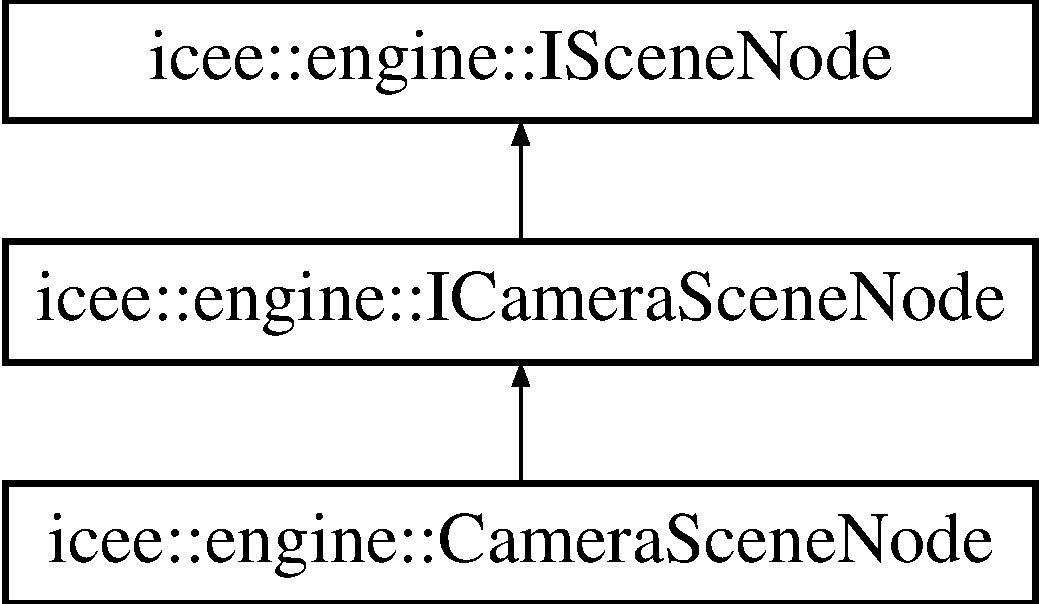
\includegraphics[height=3.000000cm]{classicee_1_1engine_1_1CameraSceneNode}
\end{center}
\end{figure}
\subsection*{Public Member Functions}
\begin{DoxyCompactItemize}
\item 
\hyperlink{classicee_1_1engine_1_1CameraSceneNode_a47864782b299cff14008cce8d586aaf0}{CameraSceneNode} ()
\item 
\hyperlink{classicee_1_1engine_1_1CameraSceneNode_a3d44228ffc351233d40f9baeb223c094}{CameraSceneNode} (\hyperlink{classvmath_1_1Vector3f}{vmath::Vector3f} position, \hyperlink{classvmath_1_1Vector3f}{vmath::Vector3f} lookAt, bool active=true)
\item 
virtual \hyperlink{classicee_1_1engine_1_1CameraSceneNode_abd6c6784830e182983ce55b08a37a1ab}{$\sim$CameraSceneNode} ()
\item 
virtual void \hyperlink{classicee_1_1engine_1_1CameraSceneNode_a230b6af4d2c61341e7146e901c25e8be}{render} ()
\item 
virtual const \hyperlink{classvmath_1_1Vector3f}{vmath::Vector3f} \& \hyperlink{classicee_1_1engine_1_1CameraSceneNode_ae6e8b374b9e726d97fe693014fca1c81}{getLookAt} ()
\item 
virtual void \hyperlink{classicee_1_1engine_1_1CameraSceneNode_a8c0d4458f9587dd4aade5e60ddeeafbe}{setLookAt} (const \hyperlink{classvmath_1_1Vector3f}{vmath::Vector3f} \&newLookAt)
\item 
virtual void \hyperlink{classicee_1_1engine_1_1CameraSceneNode_ac5d5e2204f5448375c9e830eb67e5cea}{move} (\hyperlink{classicee_1_1engine_1_1ICameraSceneNode_a47efe47a91708ebed42249f6304309ae}{MOVE\_\-DIRECTION} dir, bool enabled)
\item 
virtual void \hyperlink{classicee_1_1engine_1_1CameraSceneNode_a0f69fecc9d1153eb15fc1118a6efa28d}{rotateX} (\hyperlink{namespacecompatibility_a32a2d006ac2172c0f859370287f0104c}{float32} degrees)
\item 
virtual void \hyperlink{classicee_1_1engine_1_1CameraSceneNode_a5f2142852ab5aea21af731097a9ce9bf}{rotateY} (\hyperlink{namespacecompatibility_a32a2d006ac2172c0f859370287f0104c}{float32} degrees)
\item 
virtual void \hyperlink{classicee_1_1engine_1_1CameraSceneNode_a267404d1f0eba71120ffc7c9950bfbd4}{tick} (\hyperlink{namespacecompatibility_a32a2d006ac2172c0f859370287f0104c}{float32} time)
\end{DoxyCompactItemize}
\subsection*{Protected Member Functions}
\begin{DoxyCompactItemize}
\item 
void \hyperlink{classicee_1_1engine_1_1CameraSceneNode_ad57a1c47b456258354be6f53228fe936}{clearMovementBuffer} ()
\item 
void \hyperlink{classicee_1_1engine_1_1CameraSceneNode_a1862166f71fa916a43301842b3ca0880}{initialize} ()
\end{DoxyCompactItemize}
\subsection*{Protected Attributes}
\begin{DoxyCompactItemize}
\item 
\hyperlink{classvmath_1_1Vector3f}{vmath::Vector3f} \hyperlink{classicee_1_1engine_1_1CameraSceneNode_a00597c8ba8fc79c1bb808c64203c1da7}{lookAt\_\-}
\item 
\hyperlink{classicee_1_1engine_1_1Quaternion}{Quaternion} \hyperlink{classicee_1_1engine_1_1CameraSceneNode_a76cea9ace1709b595c18c00a62c99ccf}{rotation\_\-}
\item 
\hyperlink{namespacecompatibility_afc3ea6dfbdda98c9d2615b235b140a18}{sint32} \hyperlink{classicee_1_1engine_1_1CameraSceneNode_af34e0abb4aced603e5bc3cc1aa478f77}{prevX\_\-}
\item 
\hyperlink{namespacecompatibility_afc3ea6dfbdda98c9d2615b235b140a18}{sint32} \hyperlink{classicee_1_1engine_1_1CameraSceneNode_a6689e5b044be84a1537526497eb9da25}{prevY\_\-}
\item 
\hyperlink{namespacecompatibility_a451d9cfd3da606a663aa298356f0b5a5}{char8} \hyperlink{classicee_1_1engine_1_1CameraSceneNode_abe8f42a5901d3c4483fe8a992ba49579}{movement\_\-} \mbox{[}\hyperlink{classicee_1_1engine_1_1ICameraSceneNode_aeb9040df9d774467ed2a8c82b0f434d6}{NUM\_\-MOVE\_\-DIRECTIONS}\mbox{]}
\item 
\hyperlink{namespacecompatibility_a32a2d006ac2172c0f859370287f0104c}{float32} \hyperlink{classicee_1_1engine_1_1CameraSceneNode_a54660e34759b36a182c21df9e3d1154e}{moveSpeed\_\-}
\item 
\hyperlink{namespacecompatibility_a32a2d006ac2172c0f859370287f0104c}{float32} \hyperlink{classicee_1_1engine_1_1CameraSceneNode_a2b27e6aae2a4cd1868aeb1a274636d8b}{rotSpeed\_\-}
\item 
\hyperlink{namespacecompatibility_a32a2d006ac2172c0f859370287f0104c}{float32} \hyperlink{classicee_1_1engine_1_1CameraSceneNode_a88594483a4aa500a2ced3781a2179e78}{xRot\_\-}
\item 
\hyperlink{namespacecompatibility_a32a2d006ac2172c0f859370287f0104c}{float32} \hyperlink{classicee_1_1engine_1_1CameraSceneNode_a47c1195747ae82d087fb380fce092dbd}{yRot\_\-}
\end{DoxyCompactItemize}


\subsection{Constructor \& Destructor Documentation}
\hypertarget{classicee_1_1engine_1_1CameraSceneNode_a47864782b299cff14008cce8d586aaf0}{
\index{icee::engine::CameraSceneNode@{icee::engine::CameraSceneNode}!CameraSceneNode@{CameraSceneNode}}
\index{CameraSceneNode@{CameraSceneNode}!icee::engine::CameraSceneNode@{icee::engine::CameraSceneNode}}
\subsubsection[{CameraSceneNode}]{\setlength{\rightskip}{0pt plus 5cm}icee::engine::CameraSceneNode::CameraSceneNode (
\begin{DoxyParamCaption}
{}
\end{DoxyParamCaption}
)}}
\label{classicee_1_1engine_1_1CameraSceneNode_a47864782b299cff14008cce8d586aaf0}
\hypertarget{classicee_1_1engine_1_1CameraSceneNode_a3d44228ffc351233d40f9baeb223c094}{
\index{icee::engine::CameraSceneNode@{icee::engine::CameraSceneNode}!CameraSceneNode@{CameraSceneNode}}
\index{CameraSceneNode@{CameraSceneNode}!icee::engine::CameraSceneNode@{icee::engine::CameraSceneNode}}
\subsubsection[{CameraSceneNode}]{\setlength{\rightskip}{0pt plus 5cm}icee::engine::CameraSceneNode::CameraSceneNode (
\begin{DoxyParamCaption}
\item[{{\bf vmath::Vector3f}}]{position, }
\item[{{\bf vmath::Vector3f}}]{lookAt, }
\item[{bool}]{active = {\ttfamily true}}
\end{DoxyParamCaption}
)}}
\label{classicee_1_1engine_1_1CameraSceneNode_a3d44228ffc351233d40f9baeb223c094}
\hypertarget{classicee_1_1engine_1_1CameraSceneNode_abd6c6784830e182983ce55b08a37a1ab}{
\index{icee::engine::CameraSceneNode@{icee::engine::CameraSceneNode}!$\sim$CameraSceneNode@{$\sim$CameraSceneNode}}
\index{$\sim$CameraSceneNode@{$\sim$CameraSceneNode}!icee::engine::CameraSceneNode@{icee::engine::CameraSceneNode}}
\subsubsection[{$\sim$CameraSceneNode}]{\setlength{\rightskip}{0pt plus 5cm}icee::engine::CameraSceneNode::$\sim$CameraSceneNode (
\begin{DoxyParamCaption}
{}
\end{DoxyParamCaption}
)\hspace{0.3cm}{\ttfamily  \mbox{[}virtual\mbox{]}}}}
\label{classicee_1_1engine_1_1CameraSceneNode_abd6c6784830e182983ce55b08a37a1ab}


\subsection{Member Function Documentation}
\hypertarget{classicee_1_1engine_1_1CameraSceneNode_ad57a1c47b456258354be6f53228fe936}{
\index{icee::engine::CameraSceneNode@{icee::engine::CameraSceneNode}!clearMovementBuffer@{clearMovementBuffer}}
\index{clearMovementBuffer@{clearMovementBuffer}!icee::engine::CameraSceneNode@{icee::engine::CameraSceneNode}}
\subsubsection[{clearMovementBuffer}]{\setlength{\rightskip}{0pt plus 5cm}void icee::engine::CameraSceneNode::clearMovementBuffer (
\begin{DoxyParamCaption}
{}
\end{DoxyParamCaption}
)\hspace{0.3cm}{\ttfamily  \mbox{[}protected\mbox{]}}}}
\label{classicee_1_1engine_1_1CameraSceneNode_ad57a1c47b456258354be6f53228fe936}
\hypertarget{classicee_1_1engine_1_1CameraSceneNode_ae6e8b374b9e726d97fe693014fca1c81}{
\index{icee::engine::CameraSceneNode@{icee::engine::CameraSceneNode}!getLookAt@{getLookAt}}
\index{getLookAt@{getLookAt}!icee::engine::CameraSceneNode@{icee::engine::CameraSceneNode}}
\subsubsection[{getLookAt}]{\setlength{\rightskip}{0pt plus 5cm}const {\bf vmath::Vector3f} \& icee::engine::CameraSceneNode::getLookAt (
\begin{DoxyParamCaption}
{}
\end{DoxyParamCaption}
)\hspace{0.3cm}{\ttfamily  \mbox{[}virtual\mbox{]}}}}
\label{classicee_1_1engine_1_1CameraSceneNode_ae6e8b374b9e726d97fe693014fca1c81}


Implements \hyperlink{classicee_1_1engine_1_1ICameraSceneNode_a4cb57ce68580cac469fb3b5b0a76ce59}{icee::engine::ICameraSceneNode}.

\hypertarget{classicee_1_1engine_1_1CameraSceneNode_a1862166f71fa916a43301842b3ca0880}{
\index{icee::engine::CameraSceneNode@{icee::engine::CameraSceneNode}!initialize@{initialize}}
\index{initialize@{initialize}!icee::engine::CameraSceneNode@{icee::engine::CameraSceneNode}}
\subsubsection[{initialize}]{\setlength{\rightskip}{0pt plus 5cm}void icee::engine::CameraSceneNode::initialize (
\begin{DoxyParamCaption}
{}
\end{DoxyParamCaption}
)\hspace{0.3cm}{\ttfamily  \mbox{[}protected\mbox{]}}}}
\label{classicee_1_1engine_1_1CameraSceneNode_a1862166f71fa916a43301842b3ca0880}
\hypertarget{classicee_1_1engine_1_1CameraSceneNode_ac5d5e2204f5448375c9e830eb67e5cea}{
\index{icee::engine::CameraSceneNode@{icee::engine::CameraSceneNode}!move@{move}}
\index{move@{move}!icee::engine::CameraSceneNode@{icee::engine::CameraSceneNode}}
\subsubsection[{move}]{\setlength{\rightskip}{0pt plus 5cm}void icee::engine::CameraSceneNode::move (
\begin{DoxyParamCaption}
\item[{{\bf MOVE\_\-DIRECTION}}]{dir, }
\item[{bool}]{enabled}
\end{DoxyParamCaption}
)\hspace{0.3cm}{\ttfamily  \mbox{[}virtual\mbox{]}}}}
\label{classicee_1_1engine_1_1CameraSceneNode_ac5d5e2204f5448375c9e830eb67e5cea}


Implements \hyperlink{classicee_1_1engine_1_1ICameraSceneNode_a8f71e3eb97bbad32482358b712aa7e1a}{icee::engine::ICameraSceneNode}.

\hypertarget{classicee_1_1engine_1_1CameraSceneNode_a230b6af4d2c61341e7146e901c25e8be}{
\index{icee::engine::CameraSceneNode@{icee::engine::CameraSceneNode}!render@{render}}
\index{render@{render}!icee::engine::CameraSceneNode@{icee::engine::CameraSceneNode}}
\subsubsection[{render}]{\setlength{\rightskip}{0pt plus 5cm}void icee::engine::CameraSceneNode::render (
\begin{DoxyParamCaption}
{}
\end{DoxyParamCaption}
)\hspace{0.3cm}{\ttfamily  \mbox{[}virtual\mbox{]}}}}
\label{classicee_1_1engine_1_1CameraSceneNode_a230b6af4d2c61341e7146e901c25e8be}


Implements \hyperlink{classicee_1_1engine_1_1ICameraSceneNode_af4996793cf1cc2d0ccdf541e94ac9609}{icee::engine::ICameraSceneNode}.

\hypertarget{classicee_1_1engine_1_1CameraSceneNode_a0f69fecc9d1153eb15fc1118a6efa28d}{
\index{icee::engine::CameraSceneNode@{icee::engine::CameraSceneNode}!rotateX@{rotateX}}
\index{rotateX@{rotateX}!icee::engine::CameraSceneNode@{icee::engine::CameraSceneNode}}
\subsubsection[{rotateX}]{\setlength{\rightskip}{0pt plus 5cm}void icee::engine::CameraSceneNode::rotateX (
\begin{DoxyParamCaption}
\item[{{\bf float32}}]{degrees}
\end{DoxyParamCaption}
)\hspace{0.3cm}{\ttfamily  \mbox{[}virtual\mbox{]}}}}
\label{classicee_1_1engine_1_1CameraSceneNode_a0f69fecc9d1153eb15fc1118a6efa28d}


Implements \hyperlink{classicee_1_1engine_1_1ICameraSceneNode_a2555d17b958bd2f412139daeb73c9e27}{icee::engine::ICameraSceneNode}.

\hypertarget{classicee_1_1engine_1_1CameraSceneNode_a5f2142852ab5aea21af731097a9ce9bf}{
\index{icee::engine::CameraSceneNode@{icee::engine::CameraSceneNode}!rotateY@{rotateY}}
\index{rotateY@{rotateY}!icee::engine::CameraSceneNode@{icee::engine::CameraSceneNode}}
\subsubsection[{rotateY}]{\setlength{\rightskip}{0pt plus 5cm}void icee::engine::CameraSceneNode::rotateY (
\begin{DoxyParamCaption}
\item[{{\bf float32}}]{degrees}
\end{DoxyParamCaption}
)\hspace{0.3cm}{\ttfamily  \mbox{[}virtual\mbox{]}}}}
\label{classicee_1_1engine_1_1CameraSceneNode_a5f2142852ab5aea21af731097a9ce9bf}


Implements \hyperlink{classicee_1_1engine_1_1ICameraSceneNode_af3a40b3f41e7eac5d45acbabacac9258}{icee::engine::ICameraSceneNode}.

\hypertarget{classicee_1_1engine_1_1CameraSceneNode_a8c0d4458f9587dd4aade5e60ddeeafbe}{
\index{icee::engine::CameraSceneNode@{icee::engine::CameraSceneNode}!setLookAt@{setLookAt}}
\index{setLookAt@{setLookAt}!icee::engine::CameraSceneNode@{icee::engine::CameraSceneNode}}
\subsubsection[{setLookAt}]{\setlength{\rightskip}{0pt plus 5cm}void icee::engine::CameraSceneNode::setLookAt (
\begin{DoxyParamCaption}
\item[{const {\bf vmath::Vector3f} \&}]{newLookAt}
\end{DoxyParamCaption}
)\hspace{0.3cm}{\ttfamily  \mbox{[}virtual\mbox{]}}}}
\label{classicee_1_1engine_1_1CameraSceneNode_a8c0d4458f9587dd4aade5e60ddeeafbe}


Implements \hyperlink{classicee_1_1engine_1_1ICameraSceneNode_ad19ccccd889c46a18ff7cc8e09fda813}{icee::engine::ICameraSceneNode}.

\hypertarget{classicee_1_1engine_1_1CameraSceneNode_a267404d1f0eba71120ffc7c9950bfbd4}{
\index{icee::engine::CameraSceneNode@{icee::engine::CameraSceneNode}!tick@{tick}}
\index{tick@{tick}!icee::engine::CameraSceneNode@{icee::engine::CameraSceneNode}}
\subsubsection[{tick}]{\setlength{\rightskip}{0pt plus 5cm}void icee::engine::CameraSceneNode::tick (
\begin{DoxyParamCaption}
\item[{{\bf float32}}]{time}
\end{DoxyParamCaption}
)\hspace{0.3cm}{\ttfamily  \mbox{[}virtual\mbox{]}}}}
\label{classicee_1_1engine_1_1CameraSceneNode_a267404d1f0eba71120ffc7c9950bfbd4}


Implements \hyperlink{classicee_1_1engine_1_1ICameraSceneNode_a06dcb1ef06cfb323a088936f066d875e}{icee::engine::ICameraSceneNode}.



\subsection{Member Data Documentation}
\hypertarget{classicee_1_1engine_1_1CameraSceneNode_a00597c8ba8fc79c1bb808c64203c1da7}{
\index{icee::engine::CameraSceneNode@{icee::engine::CameraSceneNode}!lookAt\_\-@{lookAt\_\-}}
\index{lookAt\_\-@{lookAt\_\-}!icee::engine::CameraSceneNode@{icee::engine::CameraSceneNode}}
\subsubsection[{lookAt\_\-}]{\setlength{\rightskip}{0pt plus 5cm}{\bf vmath::Vector3f} {\bf icee::engine::CameraSceneNode::lookAt\_\-}\hspace{0.3cm}{\ttfamily  \mbox{[}protected\mbox{]}}}}
\label{classicee_1_1engine_1_1CameraSceneNode_a00597c8ba8fc79c1bb808c64203c1da7}
\hypertarget{classicee_1_1engine_1_1CameraSceneNode_abe8f42a5901d3c4483fe8a992ba49579}{
\index{icee::engine::CameraSceneNode@{icee::engine::CameraSceneNode}!movement\_\-@{movement\_\-}}
\index{movement\_\-@{movement\_\-}!icee::engine::CameraSceneNode@{icee::engine::CameraSceneNode}}
\subsubsection[{movement\_\-}]{\setlength{\rightskip}{0pt plus 5cm}{\bf char8} {\bf icee::engine::CameraSceneNode::movement\_\-}\mbox{[}{\bf NUM\_\-MOVE\_\-DIRECTIONS}\mbox{]}\hspace{0.3cm}{\ttfamily  \mbox{[}protected\mbox{]}}}}
\label{classicee_1_1engine_1_1CameraSceneNode_abe8f42a5901d3c4483fe8a992ba49579}
\hypertarget{classicee_1_1engine_1_1CameraSceneNode_a54660e34759b36a182c21df9e3d1154e}{
\index{icee::engine::CameraSceneNode@{icee::engine::CameraSceneNode}!moveSpeed\_\-@{moveSpeed\_\-}}
\index{moveSpeed\_\-@{moveSpeed\_\-}!icee::engine::CameraSceneNode@{icee::engine::CameraSceneNode}}
\subsubsection[{moveSpeed\_\-}]{\setlength{\rightskip}{0pt plus 5cm}{\bf float32} {\bf icee::engine::CameraSceneNode::moveSpeed\_\-}\hspace{0.3cm}{\ttfamily  \mbox{[}protected\mbox{]}}}}
\label{classicee_1_1engine_1_1CameraSceneNode_a54660e34759b36a182c21df9e3d1154e}
\hypertarget{classicee_1_1engine_1_1CameraSceneNode_af34e0abb4aced603e5bc3cc1aa478f77}{
\index{icee::engine::CameraSceneNode@{icee::engine::CameraSceneNode}!prevX\_\-@{prevX\_\-}}
\index{prevX\_\-@{prevX\_\-}!icee::engine::CameraSceneNode@{icee::engine::CameraSceneNode}}
\subsubsection[{prevX\_\-}]{\setlength{\rightskip}{0pt plus 5cm}{\bf sint32} {\bf icee::engine::CameraSceneNode::prevX\_\-}\hspace{0.3cm}{\ttfamily  \mbox{[}protected\mbox{]}}}}
\label{classicee_1_1engine_1_1CameraSceneNode_af34e0abb4aced603e5bc3cc1aa478f77}
\hypertarget{classicee_1_1engine_1_1CameraSceneNode_a6689e5b044be84a1537526497eb9da25}{
\index{icee::engine::CameraSceneNode@{icee::engine::CameraSceneNode}!prevY\_\-@{prevY\_\-}}
\index{prevY\_\-@{prevY\_\-}!icee::engine::CameraSceneNode@{icee::engine::CameraSceneNode}}
\subsubsection[{prevY\_\-}]{\setlength{\rightskip}{0pt plus 5cm}{\bf sint32} {\bf icee::engine::CameraSceneNode::prevY\_\-}\hspace{0.3cm}{\ttfamily  \mbox{[}protected\mbox{]}}}}
\label{classicee_1_1engine_1_1CameraSceneNode_a6689e5b044be84a1537526497eb9da25}
\hypertarget{classicee_1_1engine_1_1CameraSceneNode_a76cea9ace1709b595c18c00a62c99ccf}{
\index{icee::engine::CameraSceneNode@{icee::engine::CameraSceneNode}!rotation\_\-@{rotation\_\-}}
\index{rotation\_\-@{rotation\_\-}!icee::engine::CameraSceneNode@{icee::engine::CameraSceneNode}}
\subsubsection[{rotation\_\-}]{\setlength{\rightskip}{0pt plus 5cm}{\bf Quaternion} {\bf icee::engine::CameraSceneNode::rotation\_\-}\hspace{0.3cm}{\ttfamily  \mbox{[}protected\mbox{]}}}}
\label{classicee_1_1engine_1_1CameraSceneNode_a76cea9ace1709b595c18c00a62c99ccf}
\hypertarget{classicee_1_1engine_1_1CameraSceneNode_a2b27e6aae2a4cd1868aeb1a274636d8b}{
\index{icee::engine::CameraSceneNode@{icee::engine::CameraSceneNode}!rotSpeed\_\-@{rotSpeed\_\-}}
\index{rotSpeed\_\-@{rotSpeed\_\-}!icee::engine::CameraSceneNode@{icee::engine::CameraSceneNode}}
\subsubsection[{rotSpeed\_\-}]{\setlength{\rightskip}{0pt plus 5cm}{\bf float32} {\bf icee::engine::CameraSceneNode::rotSpeed\_\-}\hspace{0.3cm}{\ttfamily  \mbox{[}protected\mbox{]}}}}
\label{classicee_1_1engine_1_1CameraSceneNode_a2b27e6aae2a4cd1868aeb1a274636d8b}
\hypertarget{classicee_1_1engine_1_1CameraSceneNode_a88594483a4aa500a2ced3781a2179e78}{
\index{icee::engine::CameraSceneNode@{icee::engine::CameraSceneNode}!xRot\_\-@{xRot\_\-}}
\index{xRot\_\-@{xRot\_\-}!icee::engine::CameraSceneNode@{icee::engine::CameraSceneNode}}
\subsubsection[{xRot\_\-}]{\setlength{\rightskip}{0pt plus 5cm}{\bf float32} {\bf icee::engine::CameraSceneNode::xRot\_\-}\hspace{0.3cm}{\ttfamily  \mbox{[}protected\mbox{]}}}}
\label{classicee_1_1engine_1_1CameraSceneNode_a88594483a4aa500a2ced3781a2179e78}
\hypertarget{classicee_1_1engine_1_1CameraSceneNode_a47c1195747ae82d087fb380fce092dbd}{
\index{icee::engine::CameraSceneNode@{icee::engine::CameraSceneNode}!yRot\_\-@{yRot\_\-}}
\index{yRot\_\-@{yRot\_\-}!icee::engine::CameraSceneNode@{icee::engine::CameraSceneNode}}
\subsubsection[{yRot\_\-}]{\setlength{\rightskip}{0pt plus 5cm}{\bf float32} {\bf icee::engine::CameraSceneNode::yRot\_\-}\hspace{0.3cm}{\ttfamily  \mbox{[}protected\mbox{]}}}}
\label{classicee_1_1engine_1_1CameraSceneNode_a47c1195747ae82d087fb380fce092dbd}


The documentation for this class was generated from the following files:\begin{DoxyCompactItemize}
\item 
src/engine/\hyperlink{CameraSceneNode_8h}{CameraSceneNode.h}\item 
src/engine/\hyperlink{CameraSceneNode_8cpp}{CameraSceneNode.cpp}\end{DoxyCompactItemize}

\hypertarget{classicee_1_1engine_1_1DefaultSceneManager}{
\section{icee::engine::DefaultSceneManager Class Reference}
\label{classicee_1_1engine_1_1DefaultSceneManager}\index{icee::engine::DefaultSceneManager@{icee::engine::DefaultSceneManager}}
}


{\ttfamily \#include $<$DefaultSceneManager.h$>$}

Inheritance diagram for icee::engine::DefaultSceneManager:\begin{figure}[H]
\begin{center}
\leavevmode
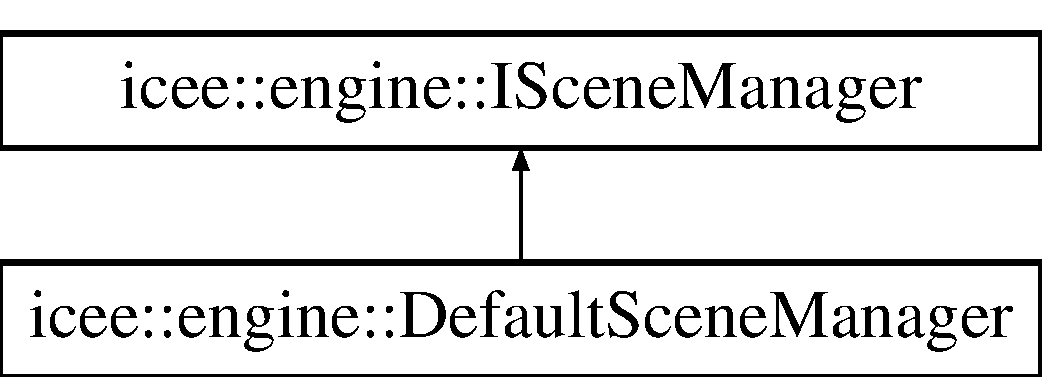
\includegraphics[height=2.000000cm]{classicee_1_1engine_1_1DefaultSceneManager}
\end{center}
\end{figure}
\subsection*{Public Member Functions}
\begin{DoxyCompactItemize}
\item 
\hyperlink{classicee_1_1engine_1_1DefaultSceneManager_a7de7cdaa3686ba77d33a96a51ebd0de4}{DefaultSceneManager} ()
\item 
virtual \hyperlink{classicee_1_1engine_1_1DefaultSceneManager_a6ff20f4bfd365794447cf7827ae22d53}{$\sim$DefaultSceneManager} ()
\item 
virtual \hyperlink{classicee_1_1engine_1_1ISceneNode}{ISceneNode} $\ast$ \hyperlink{classicee_1_1engine_1_1DefaultSceneManager_a92412af214e790045fb5890936ac37db}{addDefaultSceneNode} (const char $\ast$name, \hyperlink{classicee_1_1engine_1_1ISceneNode}{ISceneNode} $\ast$parent=0, \hyperlink{namespacecompatibility_afc3ea6dfbdda98c9d2615b235b140a18}{sint32} id=-\/1)
\item 
virtual \hyperlink{classicee_1_1engine_1_1ISceneNode}{ISceneNode} $\ast$ \hyperlink{classicee_1_1engine_1_1DefaultSceneManager_a8e19127f7542d263d8b9b34c170f40fd}{addSceneNode} (const char $\ast$name, \hyperlink{classicee_1_1engine_1_1ISceneNode}{ISceneNode} $\ast$parent=0, \hyperlink{namespacecompatibility_afc3ea6dfbdda98c9d2615b235b140a18}{sint32} id=-\/1)
\item 
virtual \hyperlink{classicee_1_1engine_1_1ICameraSceneNode}{ICameraSceneNode} $\ast$ \hyperlink{classicee_1_1engine_1_1DefaultSceneManager_ac93bba8c1d23d86ae547020e0086c5a4}{addCamera} (\hyperlink{classvmath_1_1Vector3f}{vmath::Vector3f} position, \hyperlink{classvmath_1_1Vector3f}{vmath::Vector3f} lookAt)
\item 
virtual \hyperlink{classicee_1_1engine_1_1ICameraSceneNode}{ICameraSceneNode} $\ast$ \hyperlink{classicee_1_1engine_1_1DefaultSceneManager_a75b9d066c4ff5f231e9806cfbef64caf}{addCameraFPS} (\hyperlink{classvmath_1_1Vector3f}{vmath::Vector3f} position, \hyperlink{classvmath_1_1Vector3f}{vmath::Vector3f} lookAt, \hyperlink{namespacecompatibility_a51e8fe2956b4f39fe1fae96cec0d8393}{uint32} speed, \hyperlink{namespacecompatibility_a51e8fe2956b4f39fe1fae96cec0d8393}{uint32} rotationSpeed)
\item 
virtual void \hyperlink{classicee_1_1engine_1_1DefaultSceneManager_add821d9d71b613663c391cbc37fe5f0f}{drawAll} ()
\end{DoxyCompactItemize}


\subsection{Constructor \& Destructor Documentation}
\hypertarget{classicee_1_1engine_1_1DefaultSceneManager_a7de7cdaa3686ba77d33a96a51ebd0de4}{
\index{icee::engine::DefaultSceneManager@{icee::engine::DefaultSceneManager}!DefaultSceneManager@{DefaultSceneManager}}
\index{DefaultSceneManager@{DefaultSceneManager}!icee::engine::DefaultSceneManager@{icee::engine::DefaultSceneManager}}
\subsubsection[{DefaultSceneManager}]{\setlength{\rightskip}{0pt plus 5cm}icee::engine::DefaultSceneManager::DefaultSceneManager (
\begin{DoxyParamCaption}
{}
\end{DoxyParamCaption}
)}}
\label{classicee_1_1engine_1_1DefaultSceneManager_a7de7cdaa3686ba77d33a96a51ebd0de4}
\hypertarget{classicee_1_1engine_1_1DefaultSceneManager_a6ff20f4bfd365794447cf7827ae22d53}{
\index{icee::engine::DefaultSceneManager@{icee::engine::DefaultSceneManager}!$\sim$DefaultSceneManager@{$\sim$DefaultSceneManager}}
\index{$\sim$DefaultSceneManager@{$\sim$DefaultSceneManager}!icee::engine::DefaultSceneManager@{icee::engine::DefaultSceneManager}}
\subsubsection[{$\sim$DefaultSceneManager}]{\setlength{\rightskip}{0pt plus 5cm}icee::engine::DefaultSceneManager::$\sim$DefaultSceneManager (
\begin{DoxyParamCaption}
{}
\end{DoxyParamCaption}
)\hspace{0.3cm}{\ttfamily  \mbox{[}virtual\mbox{]}}}}
\label{classicee_1_1engine_1_1DefaultSceneManager_a6ff20f4bfd365794447cf7827ae22d53}


\subsection{Member Function Documentation}
\hypertarget{classicee_1_1engine_1_1DefaultSceneManager_ac93bba8c1d23d86ae547020e0086c5a4}{
\index{icee::engine::DefaultSceneManager@{icee::engine::DefaultSceneManager}!addCamera@{addCamera}}
\index{addCamera@{addCamera}!icee::engine::DefaultSceneManager@{icee::engine::DefaultSceneManager}}
\subsubsection[{addCamera}]{\setlength{\rightskip}{0pt plus 5cm}{\bf ICameraSceneNode} $\ast$ icee::engine::DefaultSceneManager::addCamera (
\begin{DoxyParamCaption}
\item[{{\bf vmath::Vector3f}}]{position, }
\item[{{\bf vmath::Vector3f}}]{lookAt}
\end{DoxyParamCaption}
)\hspace{0.3cm}{\ttfamily  \mbox{[}virtual\mbox{]}}}}
\label{classicee_1_1engine_1_1DefaultSceneManager_ac93bba8c1d23d86ae547020e0086c5a4}


Implements \hyperlink{classicee_1_1engine_1_1ISceneManager_a2f43eae86d27ee9fd4d8964c7073cc9b}{icee::engine::ISceneManager}.

\hypertarget{classicee_1_1engine_1_1DefaultSceneManager_a75b9d066c4ff5f231e9806cfbef64caf}{
\index{icee::engine::DefaultSceneManager@{icee::engine::DefaultSceneManager}!addCameraFPS@{addCameraFPS}}
\index{addCameraFPS@{addCameraFPS}!icee::engine::DefaultSceneManager@{icee::engine::DefaultSceneManager}}
\subsubsection[{addCameraFPS}]{\setlength{\rightskip}{0pt plus 5cm}{\bf ICameraSceneNode} $\ast$ icee::engine::DefaultSceneManager::addCameraFPS (
\begin{DoxyParamCaption}
\item[{{\bf vmath::Vector3f}}]{position, }
\item[{{\bf vmath::Vector3f}}]{lookAt, }
\item[{{\bf uint32}}]{speed, }
\item[{{\bf uint32}}]{rotationSpeed}
\end{DoxyParamCaption}
)\hspace{0.3cm}{\ttfamily  \mbox{[}virtual\mbox{]}}}}
\label{classicee_1_1engine_1_1DefaultSceneManager_a75b9d066c4ff5f231e9806cfbef64caf}


Implements \hyperlink{classicee_1_1engine_1_1ISceneManager_a2165f1d59e5338aa9fd89d0242a38662}{icee::engine::ISceneManager}.

\hypertarget{classicee_1_1engine_1_1DefaultSceneManager_a92412af214e790045fb5890936ac37db}{
\index{icee::engine::DefaultSceneManager@{icee::engine::DefaultSceneManager}!addDefaultSceneNode@{addDefaultSceneNode}}
\index{addDefaultSceneNode@{addDefaultSceneNode}!icee::engine::DefaultSceneManager@{icee::engine::DefaultSceneManager}}
\subsubsection[{addDefaultSceneNode}]{\setlength{\rightskip}{0pt plus 5cm}{\bf ISceneNode} $\ast$ icee::engine::DefaultSceneManager::addDefaultSceneNode (
\begin{DoxyParamCaption}
\item[{const char $\ast$}]{name, }
\item[{{\bf ISceneNode} $\ast$}]{parent = {\ttfamily 0}, }
\item[{{\bf sint32}}]{id = {\ttfamily -\/1}}
\end{DoxyParamCaption}
)\hspace{0.3cm}{\ttfamily  \mbox{[}virtual\mbox{]}}}}
\label{classicee_1_1engine_1_1DefaultSceneManager_a92412af214e790045fb5890936ac37db}
FOR TESTING PURPOSES ONLY. 

Implements \hyperlink{classicee_1_1engine_1_1ISceneManager_afc84d5f887e850807ee36732b13c3798}{icee::engine::ISceneManager}.

\hypertarget{classicee_1_1engine_1_1DefaultSceneManager_a8e19127f7542d263d8b9b34c170f40fd}{
\index{icee::engine::DefaultSceneManager@{icee::engine::DefaultSceneManager}!addSceneNode@{addSceneNode}}
\index{addSceneNode@{addSceneNode}!icee::engine::DefaultSceneManager@{icee::engine::DefaultSceneManager}}
\subsubsection[{addSceneNode}]{\setlength{\rightskip}{0pt plus 5cm}{\bf ISceneNode} $\ast$ icee::engine::DefaultSceneManager::addSceneNode (
\begin{DoxyParamCaption}
\item[{const char $\ast$}]{name, }
\item[{{\bf ISceneNode} $\ast$}]{parent = {\ttfamily 0}, }
\item[{{\bf sint32}}]{id = {\ttfamily -\/1}}
\end{DoxyParamCaption}
)\hspace{0.3cm}{\ttfamily  \mbox{[}virtual\mbox{]}}}}
\label{classicee_1_1engine_1_1DefaultSceneManager_a8e19127f7542d263d8b9b34c170f40fd}


Implements \hyperlink{classicee_1_1engine_1_1ISceneManager_aecda2ddc8edc12f6bcf63575d988f0f1}{icee::engine::ISceneManager}.

\hypertarget{classicee_1_1engine_1_1DefaultSceneManager_add821d9d71b613663c391cbc37fe5f0f}{
\index{icee::engine::DefaultSceneManager@{icee::engine::DefaultSceneManager}!drawAll@{drawAll}}
\index{drawAll@{drawAll}!icee::engine::DefaultSceneManager@{icee::engine::DefaultSceneManager}}
\subsubsection[{drawAll}]{\setlength{\rightskip}{0pt plus 5cm}void icee::engine::DefaultSceneManager::drawAll (
\begin{DoxyParamCaption}
{}
\end{DoxyParamCaption}
)\hspace{0.3cm}{\ttfamily  \mbox{[}virtual\mbox{]}}}}
\label{classicee_1_1engine_1_1DefaultSceneManager_add821d9d71b613663c391cbc37fe5f0f}


Implements \hyperlink{classicee_1_1engine_1_1ISceneManager_a39930cf34881d0d014b41190dd356def}{icee::engine::ISceneManager}.



The documentation for this class was generated from the following files:\begin{DoxyCompactItemize}
\item 
src/engine/\hyperlink{DefaultSceneManager_8h}{DefaultSceneManager.h}\item 
src/engine/\hyperlink{DefaultSceneManager_8cpp}{DefaultSceneManager.cpp}\end{DoxyCompactItemize}

\hypertarget{classicee_1_1engine_1_1DefaultSceneNode}{
\section{icee::engine::DefaultSceneNode Class Reference}
\label{classicee_1_1engine_1_1DefaultSceneNode}\index{icee::engine::DefaultSceneNode@{icee::engine::DefaultSceneNode}}
}


{\ttfamily \#include $<$DefaultSceneNode.h$>$}

Inheritance diagram for icee::engine::DefaultSceneNode:\begin{figure}[H]
\begin{center}
\leavevmode
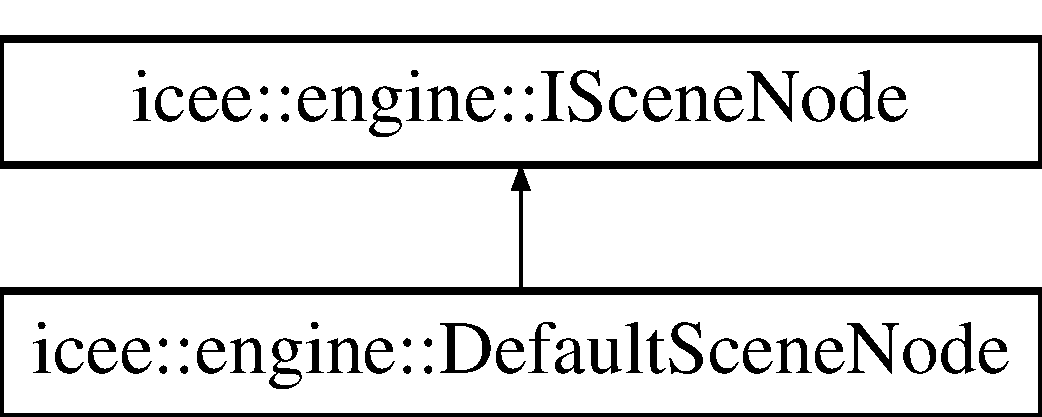
\includegraphics[height=2.000000cm]{classicee_1_1engine_1_1DefaultSceneNode}
\end{center}
\end{figure}
\subsection*{Public Member Functions}
\begin{DoxyCompactItemize}
\item 
\hyperlink{classicee_1_1engine_1_1DefaultSceneNode_ae6bf144b0f6618bb575a1563345b984d}{DefaultSceneNode} ()
\item 
virtual \hyperlink{classicee_1_1engine_1_1DefaultSceneNode_a0f7bc7135132e6d1488927b233b505a9}{$\sim$DefaultSceneNode} ()
\item 
void \hyperlink{classicee_1_1engine_1_1DefaultSceneNode_aed9092adb48382ec5423f7d2224d8fef}{render} ()
\end{DoxyCompactItemize}


\subsection{Constructor \& Destructor Documentation}
\hypertarget{classicee_1_1engine_1_1DefaultSceneNode_ae6bf144b0f6618bb575a1563345b984d}{
\index{icee::engine::DefaultSceneNode@{icee::engine::DefaultSceneNode}!DefaultSceneNode@{DefaultSceneNode}}
\index{DefaultSceneNode@{DefaultSceneNode}!icee::engine::DefaultSceneNode@{icee::engine::DefaultSceneNode}}
\subsubsection[{DefaultSceneNode}]{\setlength{\rightskip}{0pt plus 5cm}icee::engine::DefaultSceneNode::DefaultSceneNode (
\begin{DoxyParamCaption}
{}
\end{DoxyParamCaption}
)}}
\label{classicee_1_1engine_1_1DefaultSceneNode_ae6bf144b0f6618bb575a1563345b984d}
\hypertarget{classicee_1_1engine_1_1DefaultSceneNode_a0f7bc7135132e6d1488927b233b505a9}{
\index{icee::engine::DefaultSceneNode@{icee::engine::DefaultSceneNode}!$\sim$DefaultSceneNode@{$\sim$DefaultSceneNode}}
\index{$\sim$DefaultSceneNode@{$\sim$DefaultSceneNode}!icee::engine::DefaultSceneNode@{icee::engine::DefaultSceneNode}}
\subsubsection[{$\sim$DefaultSceneNode}]{\setlength{\rightskip}{0pt plus 5cm}icee::engine::DefaultSceneNode::$\sim$DefaultSceneNode (
\begin{DoxyParamCaption}
{}
\end{DoxyParamCaption}
)\hspace{0.3cm}{\ttfamily  \mbox{[}virtual\mbox{]}}}}
\label{classicee_1_1engine_1_1DefaultSceneNode_a0f7bc7135132e6d1488927b233b505a9}


\subsection{Member Function Documentation}
\hypertarget{classicee_1_1engine_1_1DefaultSceneNode_aed9092adb48382ec5423f7d2224d8fef}{
\index{icee::engine::DefaultSceneNode@{icee::engine::DefaultSceneNode}!render@{render}}
\index{render@{render}!icee::engine::DefaultSceneNode@{icee::engine::DefaultSceneNode}}
\subsubsection[{render}]{\setlength{\rightskip}{0pt plus 5cm}void icee::engine::DefaultSceneNode::render (
\begin{DoxyParamCaption}
{}
\end{DoxyParamCaption}
)\hspace{0.3cm}{\ttfamily  \mbox{[}virtual\mbox{]}}}}
\label{classicee_1_1engine_1_1DefaultSceneNode_aed9092adb48382ec5423f7d2224d8fef}


Implements \hyperlink{classicee_1_1engine_1_1ISceneNode_a2951ecb91b29bcc74d992de4880daa0f}{icee::engine::ISceneNode}.



The documentation for this class was generated from the following files:\begin{DoxyCompactItemize}
\item 
src/engine/\hyperlink{DefaultSceneNode_8h}{DefaultSceneNode.h}\item 
src/engine/\hyperlink{DefaultSceneNode_8cpp}{DefaultSceneNode.cpp}\end{DoxyCompactItemize}

\hypertarget{classicee_1_1engine_1_1ICameraSceneNode}{
\section{icee::engine::ICameraSceneNode Class Reference}
\label{classicee_1_1engine_1_1ICameraSceneNode}\index{icee::engine::ICameraSceneNode@{icee::engine::ICameraSceneNode}}
}


{\ttfamily \#include $<$ICameraSceneNode.h$>$}

Inheritance diagram for icee::engine::ICameraSceneNode:\begin{figure}[H]
\begin{center}
\leavevmode
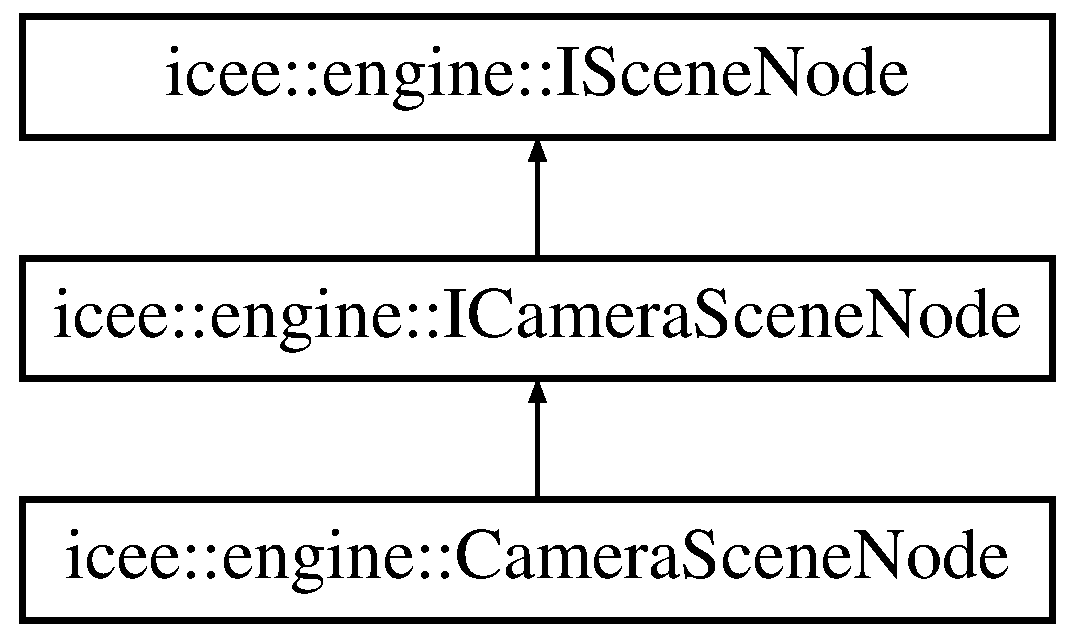
\includegraphics[height=3.000000cm]{classicee_1_1engine_1_1ICameraSceneNode}
\end{center}
\end{figure}
\subsection*{Public Types}
\begin{DoxyCompactItemize}
\item 
enum \hyperlink{classicee_1_1engine_1_1ICameraSceneNode_a47efe47a91708ebed42249f6304309ae}{MOVE\_\-DIRECTION} \{ \hyperlink{classicee_1_1engine_1_1ICameraSceneNode_a47efe47a91708ebed42249f6304309aea4b03ae2f86d7021eeb3bfb29cae8008a}{MOVE\_\-DIR\_\-FORWARD} =  0, 
\hyperlink{classicee_1_1engine_1_1ICameraSceneNode_a47efe47a91708ebed42249f6304309aead6aeef956bcf2e8416ccc78acd5ec64e}{MOVE\_\-DIR\_\-BACKWARD} =  1, 
\hyperlink{classicee_1_1engine_1_1ICameraSceneNode_a47efe47a91708ebed42249f6304309aea44938439731c5cc9022d17825724c372}{MOVE\_\-DIR\_\-LEFT} =  2, 
\hyperlink{classicee_1_1engine_1_1ICameraSceneNode_a47efe47a91708ebed42249f6304309aea7a1cbc442f614f40bc382413b7070f50}{MOVE\_\-DIR\_\-RIGHT} =  3
 \}
\item 
enum \hyperlink{classicee_1_1engine_1_1ICameraSceneNode_ad7a023986a81f07295135d249c0f00aa}{LOOK\_\-DIRECTION} \{ \hyperlink{classicee_1_1engine_1_1ICameraSceneNode_ad7a023986a81f07295135d249c0f00aaab2871197cec134720ca9207cfce48bf4}{LOOK\_\-DIR\_\-UP} =  0, 
\hyperlink{classicee_1_1engine_1_1ICameraSceneNode_ad7a023986a81f07295135d249c0f00aaa92059eac70f7a3d72ecf26cbe5420ab5}{LOOK\_\-DIR\_\-DOWN} =  1, 
\hyperlink{classicee_1_1engine_1_1ICameraSceneNode_ad7a023986a81f07295135d249c0f00aaacc9a232b8da0c5a96d16d87ab7872d29}{LOOK\_\-DIR\_\-LEFT} =  2, 
\hyperlink{classicee_1_1engine_1_1ICameraSceneNode_ad7a023986a81f07295135d249c0f00aaac6fb21864521bba688ea3565c8ddbf99}{LOOK\_\-DIR\_\-RIGHT} =  3
 \}
\end{DoxyCompactItemize}
\subsection*{Public Member Functions}
\begin{DoxyCompactItemize}
\item 
virtual \hyperlink{classicee_1_1engine_1_1ICameraSceneNode_a6a5b592cf16937061d79ba6be5d0f966}{$\sim$ICameraSceneNode} ()
\item 
virtual const \hyperlink{classvmath_1_1Vector3f}{vmath::Vector3f} \& \hyperlink{classicee_1_1engine_1_1ICameraSceneNode_a4cb57ce68580cac469fb3b5b0a76ce59}{getLookAt} ()=0
\item 
virtual void \hyperlink{classicee_1_1engine_1_1ICameraSceneNode_ad19ccccd889c46a18ff7cc8e09fda813}{setLookAt} (const \hyperlink{classvmath_1_1Vector3f}{vmath::Vector3f} \&newLookAt)=0
\item 
virtual void \hyperlink{classicee_1_1engine_1_1ICameraSceneNode_a8f71e3eb97bbad32482358b712aa7e1a}{move} (\hyperlink{classicee_1_1engine_1_1ICameraSceneNode_a47efe47a91708ebed42249f6304309ae}{MOVE\_\-DIRECTION} dir, bool enabled)=0
\item 
virtual void \hyperlink{classicee_1_1engine_1_1ICameraSceneNode_a2555d17b958bd2f412139daeb73c9e27}{rotateX} (\hyperlink{namespacecompatibility_a32a2d006ac2172c0f859370287f0104c}{float32} degrees)=0
\item 
virtual void \hyperlink{classicee_1_1engine_1_1ICameraSceneNode_af3a40b3f41e7eac5d45acbabacac9258}{rotateY} (\hyperlink{namespacecompatibility_a32a2d006ac2172c0f859370287f0104c}{float32} degrees)=0
\item 
virtual void \hyperlink{classicee_1_1engine_1_1ICameraSceneNode_a06dcb1ef06cfb323a088936f066d875e}{tick} (\hyperlink{namespacecompatibility_a32a2d006ac2172c0f859370287f0104c}{float32} time)=0
\item 
virtual void \hyperlink{classicee_1_1engine_1_1ICameraSceneNode_af4996793cf1cc2d0ccdf541e94ac9609}{render} ()=0
\end{DoxyCompactItemize}
\subsection*{Static Public Attributes}
\begin{DoxyCompactItemize}
\item 
static const \hyperlink{namespacecompatibility_a51e8fe2956b4f39fe1fae96cec0d8393}{uint32} \hyperlink{classicee_1_1engine_1_1ICameraSceneNode_aeb9040df9d774467ed2a8c82b0f434d6}{NUM\_\-MOVE\_\-DIRECTIONS} = 4
\item 
static const \hyperlink{namespacecompatibility_a51e8fe2956b4f39fe1fae96cec0d8393}{uint32} \hyperlink{classicee_1_1engine_1_1ICameraSceneNode_a2447c4155f864c390fe95f8d227bc404}{NUM\_\-LOOK\_\-DIRECTIONS} = 4
\end{DoxyCompactItemize}


\subsection{Member Enumeration Documentation}
\hypertarget{classicee_1_1engine_1_1ICameraSceneNode_ad7a023986a81f07295135d249c0f00aa}{
\index{icee::engine::ICameraSceneNode@{icee::engine::ICameraSceneNode}!LOOK\_\-DIRECTION@{LOOK\_\-DIRECTION}}
\index{LOOK\_\-DIRECTION@{LOOK\_\-DIRECTION}!icee::engine::ICameraSceneNode@{icee::engine::ICameraSceneNode}}
\subsubsection[{LOOK\_\-DIRECTION}]{\setlength{\rightskip}{0pt plus 5cm}enum {\bf icee::engine::ICameraSceneNode::LOOK\_\-DIRECTION}}}
\label{classicee_1_1engine_1_1ICameraSceneNode_ad7a023986a81f07295135d249c0f00aa}
\begin{Desc}
\item[Enumerator: ]\par
\begin{description}
\index{LOOK\_\-DIR\_\-UP@{LOOK\_\-DIR\_\-UP}!icee::engine::ICameraSceneNode@{icee::engine::ICameraSceneNode}}\index{icee::engine::ICameraSceneNode@{icee::engine::ICameraSceneNode}!LOOK\_\-DIR\_\-UP@{LOOK\_\-DIR\_\-UP}}\item[{\em 
\hypertarget{classicee_1_1engine_1_1ICameraSceneNode_ad7a023986a81f07295135d249c0f00aaab2871197cec134720ca9207cfce48bf4}{
LOOK\_\-DIR\_\-UP}
\label{classicee_1_1engine_1_1ICameraSceneNode_ad7a023986a81f07295135d249c0f00aaab2871197cec134720ca9207cfce48bf4}
}]\index{LOOK\_\-DIR\_\-DOWN@{LOOK\_\-DIR\_\-DOWN}!icee::engine::ICameraSceneNode@{icee::engine::ICameraSceneNode}}\index{icee::engine::ICameraSceneNode@{icee::engine::ICameraSceneNode}!LOOK\_\-DIR\_\-DOWN@{LOOK\_\-DIR\_\-DOWN}}\item[{\em 
\hypertarget{classicee_1_1engine_1_1ICameraSceneNode_ad7a023986a81f07295135d249c0f00aaa92059eac70f7a3d72ecf26cbe5420ab5}{
LOOK\_\-DIR\_\-DOWN}
\label{classicee_1_1engine_1_1ICameraSceneNode_ad7a023986a81f07295135d249c0f00aaa92059eac70f7a3d72ecf26cbe5420ab5}
}]\index{LOOK\_\-DIR\_\-LEFT@{LOOK\_\-DIR\_\-LEFT}!icee::engine::ICameraSceneNode@{icee::engine::ICameraSceneNode}}\index{icee::engine::ICameraSceneNode@{icee::engine::ICameraSceneNode}!LOOK\_\-DIR\_\-LEFT@{LOOK\_\-DIR\_\-LEFT}}\item[{\em 
\hypertarget{classicee_1_1engine_1_1ICameraSceneNode_ad7a023986a81f07295135d249c0f00aaacc9a232b8da0c5a96d16d87ab7872d29}{
LOOK\_\-DIR\_\-LEFT}
\label{classicee_1_1engine_1_1ICameraSceneNode_ad7a023986a81f07295135d249c0f00aaacc9a232b8da0c5a96d16d87ab7872d29}
}]\index{LOOK\_\-DIR\_\-RIGHT@{LOOK\_\-DIR\_\-RIGHT}!icee::engine::ICameraSceneNode@{icee::engine::ICameraSceneNode}}\index{icee::engine::ICameraSceneNode@{icee::engine::ICameraSceneNode}!LOOK\_\-DIR\_\-RIGHT@{LOOK\_\-DIR\_\-RIGHT}}\item[{\em 
\hypertarget{classicee_1_1engine_1_1ICameraSceneNode_ad7a023986a81f07295135d249c0f00aaac6fb21864521bba688ea3565c8ddbf99}{
LOOK\_\-DIR\_\-RIGHT}
\label{classicee_1_1engine_1_1ICameraSceneNode_ad7a023986a81f07295135d249c0f00aaac6fb21864521bba688ea3565c8ddbf99}
}]\end{description}
\end{Desc}

\hypertarget{classicee_1_1engine_1_1ICameraSceneNode_a47efe47a91708ebed42249f6304309ae}{
\index{icee::engine::ICameraSceneNode@{icee::engine::ICameraSceneNode}!MOVE\_\-DIRECTION@{MOVE\_\-DIRECTION}}
\index{MOVE\_\-DIRECTION@{MOVE\_\-DIRECTION}!icee::engine::ICameraSceneNode@{icee::engine::ICameraSceneNode}}
\subsubsection[{MOVE\_\-DIRECTION}]{\setlength{\rightskip}{0pt plus 5cm}enum {\bf icee::engine::ICameraSceneNode::MOVE\_\-DIRECTION}}}
\label{classicee_1_1engine_1_1ICameraSceneNode_a47efe47a91708ebed42249f6304309ae}
\begin{Desc}
\item[Enumerator: ]\par
\begin{description}
\index{MOVE\_\-DIR\_\-FORWARD@{MOVE\_\-DIR\_\-FORWARD}!icee::engine::ICameraSceneNode@{icee::engine::ICameraSceneNode}}\index{icee::engine::ICameraSceneNode@{icee::engine::ICameraSceneNode}!MOVE\_\-DIR\_\-FORWARD@{MOVE\_\-DIR\_\-FORWARD}}\item[{\em 
\hypertarget{classicee_1_1engine_1_1ICameraSceneNode_a47efe47a91708ebed42249f6304309aea4b03ae2f86d7021eeb3bfb29cae8008a}{
MOVE\_\-DIR\_\-FORWARD}
\label{classicee_1_1engine_1_1ICameraSceneNode_a47efe47a91708ebed42249f6304309aea4b03ae2f86d7021eeb3bfb29cae8008a}
}]\index{MOVE\_\-DIR\_\-BACKWARD@{MOVE\_\-DIR\_\-BACKWARD}!icee::engine::ICameraSceneNode@{icee::engine::ICameraSceneNode}}\index{icee::engine::ICameraSceneNode@{icee::engine::ICameraSceneNode}!MOVE\_\-DIR\_\-BACKWARD@{MOVE\_\-DIR\_\-BACKWARD}}\item[{\em 
\hypertarget{classicee_1_1engine_1_1ICameraSceneNode_a47efe47a91708ebed42249f6304309aead6aeef956bcf2e8416ccc78acd5ec64e}{
MOVE\_\-DIR\_\-BACKWARD}
\label{classicee_1_1engine_1_1ICameraSceneNode_a47efe47a91708ebed42249f6304309aead6aeef956bcf2e8416ccc78acd5ec64e}
}]\index{MOVE\_\-DIR\_\-LEFT@{MOVE\_\-DIR\_\-LEFT}!icee::engine::ICameraSceneNode@{icee::engine::ICameraSceneNode}}\index{icee::engine::ICameraSceneNode@{icee::engine::ICameraSceneNode}!MOVE\_\-DIR\_\-LEFT@{MOVE\_\-DIR\_\-LEFT}}\item[{\em 
\hypertarget{classicee_1_1engine_1_1ICameraSceneNode_a47efe47a91708ebed42249f6304309aea44938439731c5cc9022d17825724c372}{
MOVE\_\-DIR\_\-LEFT}
\label{classicee_1_1engine_1_1ICameraSceneNode_a47efe47a91708ebed42249f6304309aea44938439731c5cc9022d17825724c372}
}]\index{MOVE\_\-DIR\_\-RIGHT@{MOVE\_\-DIR\_\-RIGHT}!icee::engine::ICameraSceneNode@{icee::engine::ICameraSceneNode}}\index{icee::engine::ICameraSceneNode@{icee::engine::ICameraSceneNode}!MOVE\_\-DIR\_\-RIGHT@{MOVE\_\-DIR\_\-RIGHT}}\item[{\em 
\hypertarget{classicee_1_1engine_1_1ICameraSceneNode_a47efe47a91708ebed42249f6304309aea7a1cbc442f614f40bc382413b7070f50}{
MOVE\_\-DIR\_\-RIGHT}
\label{classicee_1_1engine_1_1ICameraSceneNode_a47efe47a91708ebed42249f6304309aea7a1cbc442f614f40bc382413b7070f50}
}]\end{description}
\end{Desc}



\subsection{Constructor \& Destructor Documentation}
\hypertarget{classicee_1_1engine_1_1ICameraSceneNode_a6a5b592cf16937061d79ba6be5d0f966}{
\index{icee::engine::ICameraSceneNode@{icee::engine::ICameraSceneNode}!$\sim$ICameraSceneNode@{$\sim$ICameraSceneNode}}
\index{$\sim$ICameraSceneNode@{$\sim$ICameraSceneNode}!icee::engine::ICameraSceneNode@{icee::engine::ICameraSceneNode}}
\subsubsection[{$\sim$ICameraSceneNode}]{\setlength{\rightskip}{0pt plus 5cm}virtual icee::engine::ICameraSceneNode::$\sim$ICameraSceneNode (
\begin{DoxyParamCaption}
{}
\end{DoxyParamCaption}
)\hspace{0.3cm}{\ttfamily  \mbox{[}inline, virtual\mbox{]}}}}
\label{classicee_1_1engine_1_1ICameraSceneNode_a6a5b592cf16937061d79ba6be5d0f966}


\subsection{Member Function Documentation}
\hypertarget{classicee_1_1engine_1_1ICameraSceneNode_a4cb57ce68580cac469fb3b5b0a76ce59}{
\index{icee::engine::ICameraSceneNode@{icee::engine::ICameraSceneNode}!getLookAt@{getLookAt}}
\index{getLookAt@{getLookAt}!icee::engine::ICameraSceneNode@{icee::engine::ICameraSceneNode}}
\subsubsection[{getLookAt}]{\setlength{\rightskip}{0pt plus 5cm}virtual const {\bf vmath::Vector3f}\& icee::engine::ICameraSceneNode::getLookAt (
\begin{DoxyParamCaption}
{}
\end{DoxyParamCaption}
)\hspace{0.3cm}{\ttfamily  \mbox{[}pure virtual\mbox{]}}}}
\label{classicee_1_1engine_1_1ICameraSceneNode_a4cb57ce68580cac469fb3b5b0a76ce59}


Implemented in \hyperlink{classicee_1_1engine_1_1CameraSceneNode_ae6e8b374b9e726d97fe693014fca1c81}{icee::engine::CameraSceneNode}.

\hypertarget{classicee_1_1engine_1_1ICameraSceneNode_a8f71e3eb97bbad32482358b712aa7e1a}{
\index{icee::engine::ICameraSceneNode@{icee::engine::ICameraSceneNode}!move@{move}}
\index{move@{move}!icee::engine::ICameraSceneNode@{icee::engine::ICameraSceneNode}}
\subsubsection[{move}]{\setlength{\rightskip}{0pt plus 5cm}virtual void icee::engine::ICameraSceneNode::move (
\begin{DoxyParamCaption}
\item[{{\bf MOVE\_\-DIRECTION}}]{dir, }
\item[{bool}]{enabled}
\end{DoxyParamCaption}
)\hspace{0.3cm}{\ttfamily  \mbox{[}pure virtual\mbox{]}}}}
\label{classicee_1_1engine_1_1ICameraSceneNode_a8f71e3eb97bbad32482358b712aa7e1a}


Implemented in \hyperlink{classicee_1_1engine_1_1CameraSceneNode_ac5d5e2204f5448375c9e830eb67e5cea}{icee::engine::CameraSceneNode}.

\hypertarget{classicee_1_1engine_1_1ICameraSceneNode_af4996793cf1cc2d0ccdf541e94ac9609}{
\index{icee::engine::ICameraSceneNode@{icee::engine::ICameraSceneNode}!render@{render}}
\index{render@{render}!icee::engine::ICameraSceneNode@{icee::engine::ICameraSceneNode}}
\subsubsection[{render}]{\setlength{\rightskip}{0pt plus 5cm}virtual void icee::engine::ICameraSceneNode::render (
\begin{DoxyParamCaption}
{}
\end{DoxyParamCaption}
)\hspace{0.3cm}{\ttfamily  \mbox{[}pure virtual\mbox{]}}}}
\label{classicee_1_1engine_1_1ICameraSceneNode_af4996793cf1cc2d0ccdf541e94ac9609}


Implements \hyperlink{classicee_1_1engine_1_1ISceneNode_a2951ecb91b29bcc74d992de4880daa0f}{icee::engine::ISceneNode}.



Implemented in \hyperlink{classicee_1_1engine_1_1CameraSceneNode_a230b6af4d2c61341e7146e901c25e8be}{icee::engine::CameraSceneNode}.

\hypertarget{classicee_1_1engine_1_1ICameraSceneNode_a2555d17b958bd2f412139daeb73c9e27}{
\index{icee::engine::ICameraSceneNode@{icee::engine::ICameraSceneNode}!rotateX@{rotateX}}
\index{rotateX@{rotateX}!icee::engine::ICameraSceneNode@{icee::engine::ICameraSceneNode}}
\subsubsection[{rotateX}]{\setlength{\rightskip}{0pt plus 5cm}virtual void icee::engine::ICameraSceneNode::rotateX (
\begin{DoxyParamCaption}
\item[{{\bf float32}}]{degrees}
\end{DoxyParamCaption}
)\hspace{0.3cm}{\ttfamily  \mbox{[}pure virtual\mbox{]}}}}
\label{classicee_1_1engine_1_1ICameraSceneNode_a2555d17b958bd2f412139daeb73c9e27}


Implemented in \hyperlink{classicee_1_1engine_1_1CameraSceneNode_a0f69fecc9d1153eb15fc1118a6efa28d}{icee::engine::CameraSceneNode}.

\hypertarget{classicee_1_1engine_1_1ICameraSceneNode_af3a40b3f41e7eac5d45acbabacac9258}{
\index{icee::engine::ICameraSceneNode@{icee::engine::ICameraSceneNode}!rotateY@{rotateY}}
\index{rotateY@{rotateY}!icee::engine::ICameraSceneNode@{icee::engine::ICameraSceneNode}}
\subsubsection[{rotateY}]{\setlength{\rightskip}{0pt plus 5cm}virtual void icee::engine::ICameraSceneNode::rotateY (
\begin{DoxyParamCaption}
\item[{{\bf float32}}]{degrees}
\end{DoxyParamCaption}
)\hspace{0.3cm}{\ttfamily  \mbox{[}pure virtual\mbox{]}}}}
\label{classicee_1_1engine_1_1ICameraSceneNode_af3a40b3f41e7eac5d45acbabacac9258}


Implemented in \hyperlink{classicee_1_1engine_1_1CameraSceneNode_a5f2142852ab5aea21af731097a9ce9bf}{icee::engine::CameraSceneNode}.

\hypertarget{classicee_1_1engine_1_1ICameraSceneNode_ad19ccccd889c46a18ff7cc8e09fda813}{
\index{icee::engine::ICameraSceneNode@{icee::engine::ICameraSceneNode}!setLookAt@{setLookAt}}
\index{setLookAt@{setLookAt}!icee::engine::ICameraSceneNode@{icee::engine::ICameraSceneNode}}
\subsubsection[{setLookAt}]{\setlength{\rightskip}{0pt plus 5cm}virtual void icee::engine::ICameraSceneNode::setLookAt (
\begin{DoxyParamCaption}
\item[{const {\bf vmath::Vector3f} \&}]{newLookAt}
\end{DoxyParamCaption}
)\hspace{0.3cm}{\ttfamily  \mbox{[}pure virtual\mbox{]}}}}
\label{classicee_1_1engine_1_1ICameraSceneNode_ad19ccccd889c46a18ff7cc8e09fda813}


Implemented in \hyperlink{classicee_1_1engine_1_1CameraSceneNode_a8c0d4458f9587dd4aade5e60ddeeafbe}{icee::engine::CameraSceneNode}.

\hypertarget{classicee_1_1engine_1_1ICameraSceneNode_a06dcb1ef06cfb323a088936f066d875e}{
\index{icee::engine::ICameraSceneNode@{icee::engine::ICameraSceneNode}!tick@{tick}}
\index{tick@{tick}!icee::engine::ICameraSceneNode@{icee::engine::ICameraSceneNode}}
\subsubsection[{tick}]{\setlength{\rightskip}{0pt plus 5cm}virtual void icee::engine::ICameraSceneNode::tick (
\begin{DoxyParamCaption}
\item[{{\bf float32}}]{time}
\end{DoxyParamCaption}
)\hspace{0.3cm}{\ttfamily  \mbox{[}pure virtual\mbox{]}}}}
\label{classicee_1_1engine_1_1ICameraSceneNode_a06dcb1ef06cfb323a088936f066d875e}


Implemented in \hyperlink{classicee_1_1engine_1_1CameraSceneNode_a267404d1f0eba71120ffc7c9950bfbd4}{icee::engine::CameraSceneNode}.



\subsection{Member Data Documentation}
\hypertarget{classicee_1_1engine_1_1ICameraSceneNode_a2447c4155f864c390fe95f8d227bc404}{
\index{icee::engine::ICameraSceneNode@{icee::engine::ICameraSceneNode}!NUM\_\-LOOK\_\-DIRECTIONS@{NUM\_\-LOOK\_\-DIRECTIONS}}
\index{NUM\_\-LOOK\_\-DIRECTIONS@{NUM\_\-LOOK\_\-DIRECTIONS}!icee::engine::ICameraSceneNode@{icee::engine::ICameraSceneNode}}
\subsubsection[{NUM\_\-LOOK\_\-DIRECTIONS}]{\setlength{\rightskip}{0pt plus 5cm}const {\bf uint32} {\bf icee::engine::ICameraSceneNode::NUM\_\-LOOK\_\-DIRECTIONS} = 4\hspace{0.3cm}{\ttfamily  \mbox{[}static\mbox{]}}}}
\label{classicee_1_1engine_1_1ICameraSceneNode_a2447c4155f864c390fe95f8d227bc404}
\hypertarget{classicee_1_1engine_1_1ICameraSceneNode_aeb9040df9d774467ed2a8c82b0f434d6}{
\index{icee::engine::ICameraSceneNode@{icee::engine::ICameraSceneNode}!NUM\_\-MOVE\_\-DIRECTIONS@{NUM\_\-MOVE\_\-DIRECTIONS}}
\index{NUM\_\-MOVE\_\-DIRECTIONS@{NUM\_\-MOVE\_\-DIRECTIONS}!icee::engine::ICameraSceneNode@{icee::engine::ICameraSceneNode}}
\subsubsection[{NUM\_\-MOVE\_\-DIRECTIONS}]{\setlength{\rightskip}{0pt plus 5cm}const {\bf uint32} {\bf icee::engine::ICameraSceneNode::NUM\_\-MOVE\_\-DIRECTIONS} = 4\hspace{0.3cm}{\ttfamily  \mbox{[}static\mbox{]}}}}
\label{classicee_1_1engine_1_1ICameraSceneNode_aeb9040df9d774467ed2a8c82b0f434d6}


The documentation for this class was generated from the following file:\begin{DoxyCompactItemize}
\item 
src/engine/\hyperlink{ICameraSceneNode_8h}{ICameraSceneNode.h}\end{DoxyCompactItemize}

\hypertarget{classicee_1_1engine_1_1IceGLWindow}{
\section{icee::engine::IceGLWindow Class Reference}
\label{classicee_1_1engine_1_1IceGLWindow}\index{icee::engine::IceGLWindow@{icee::engine::IceGLWindow}}
}


{\ttfamily \#include $<$IceGLWindow.h$>$}

Inheritance diagram for icee::engine::IceGLWindow:\begin{figure}[H]
\begin{center}
\leavevmode
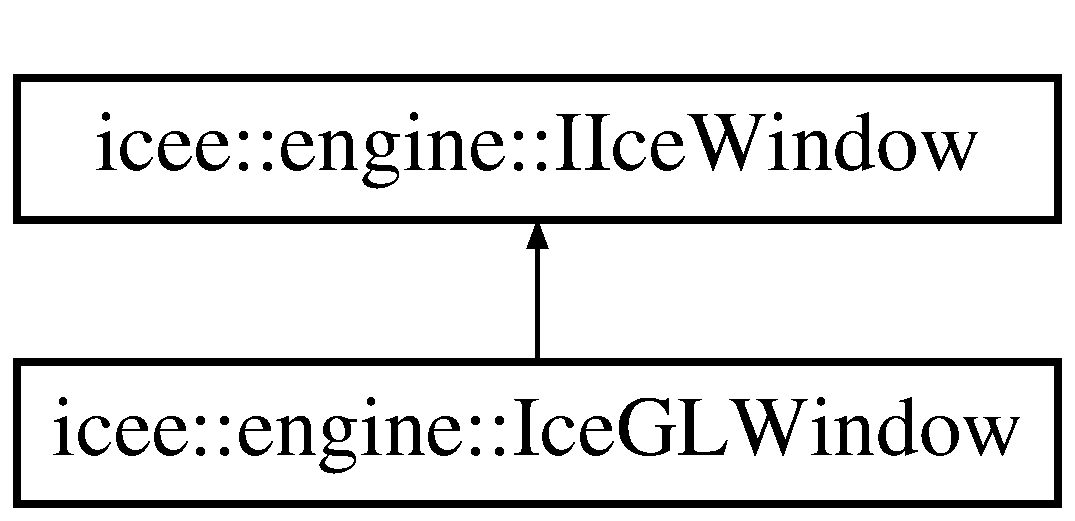
\includegraphics[height=2.000000cm]{classicee_1_1engine_1_1IceGLWindow}
\end{center}
\end{figure}
\subsection*{Public Member Functions}
\begin{DoxyCompactItemize}
\item 
\hyperlink{classicee_1_1engine_1_1IceGLWindow_a64f8470f65c29040b7abdf6aba331e21}{IceGLWindow} ()
\item 
virtual \hyperlink{classicee_1_1engine_1_1IceGLWindow_a990d8f38eacca70830b9b7e1b59083d0}{$\sim$IceGLWindow} ()
\item 
virtual void $\ast$ \hyperlink{classicee_1_1engine_1_1IceGLWindow_af041e4ce63d97bb82867dfc03b12c0d7}{getWindowPointer} ()
\item 
virtual void \hyperlink{classicee_1_1engine_1_1IceGLWindow_a130ecba0ab9ae8d73e86726232be532a}{resize} (\hyperlink{namespacecompatibility_a51e8fe2956b4f39fe1fae96cec0d8393}{uint32} width, \hyperlink{namespacecompatibility_a51e8fe2956b4f39fe1fae96cec0d8393}{uint32} height)
\item 
virtual \hyperlink{namespacecompatibility_afc3ea6dfbdda98c9d2615b235b140a18}{sint32} \hyperlink{classicee_1_1engine_1_1IceGLWindow_a58bbfb06402448f1e7791d699ce084b3}{initialize} ()
\item 
virtual void \hyperlink{classicee_1_1engine_1_1IceGLWindow_ad6fa5825e2205d7f2a93da5bfd0dfbcb}{destroy} ()
\item 
\hyperlink{namespacecompatibility_afc3ea6dfbdda98c9d2615b235b140a18}{sint32} \hyperlink{classicee_1_1engine_1_1IceGLWindow_a6b1aa21ff2b90a665647df912166d33a}{handleEvents} ()
\item 
virtual void \hyperlink{classicee_1_1engine_1_1IceGLWindow_a766acd9860c1d9160706f168105e72a5}{render} ()
\item 
virtual bool \hyperlink{classicee_1_1engine_1_1IceGLWindow_ab686b165d4359e0666dc2214e3d96117}{blah} ()
\item 
virtual \hyperlink{namespacecompatibility_a51e8fe2956b4f39fe1fae96cec0d8393}{uint32} \hyperlink{classicee_1_1engine_1_1IceGLWindow_addcb63afdfd392ded686eae4e8fe5f03}{getWidth} ()
\item 
virtual \hyperlink{namespacecompatibility_a51e8fe2956b4f39fe1fae96cec0d8393}{uint32} \hyperlink{classicee_1_1engine_1_1IceGLWindow_abd215ddc49ebe774a942c27c46b7acee}{getHeight} ()
\item 
virtual \hyperlink{namespacecompatibility_a51e8fe2956b4f39fe1fae96cec0d8393}{uint32} \hyperlink{classicee_1_1engine_1_1IceGLWindow_a979ae0c471ae0b216ad8762a0c3cfe2a}{getDepth} ()
\item 
virtual \hyperlink{classicee_1_1engine_1_1ISceneManager}{ISceneManager} $\ast$ \hyperlink{classicee_1_1engine_1_1IceGLWindow_a5b181115911d51611e2ba50fddc6f8d9}{getSceneManager} ()
\end{DoxyCompactItemize}
\subsection*{Protected Attributes}
\begin{DoxyCompactItemize}
\item 
\hyperlink{classicee_1_1engine_1_1DefaultSceneManager}{DefaultSceneManager} $\ast$ \hyperlink{classicee_1_1engine_1_1IceGLWindow_aa829f931af2426ba4f136f1629f401ed}{sMgr\_\-}
\end{DoxyCompactItemize}


\subsection{Constructor \& Destructor Documentation}
\hypertarget{classicee_1_1engine_1_1IceGLWindow_a64f8470f65c29040b7abdf6aba331e21}{
\index{icee::engine::IceGLWindow@{icee::engine::IceGLWindow}!IceGLWindow@{IceGLWindow}}
\index{IceGLWindow@{IceGLWindow}!icee::engine::IceGLWindow@{icee::engine::IceGLWindow}}
\subsubsection[{IceGLWindow}]{\setlength{\rightskip}{0pt plus 5cm}icee::engine::IceGLWindow::IceGLWindow (
\begin{DoxyParamCaption}
{}
\end{DoxyParamCaption}
)}}
\label{classicee_1_1engine_1_1IceGLWindow_a64f8470f65c29040b7abdf6aba331e21}
\hypertarget{classicee_1_1engine_1_1IceGLWindow_a990d8f38eacca70830b9b7e1b59083d0}{
\index{icee::engine::IceGLWindow@{icee::engine::IceGLWindow}!$\sim$IceGLWindow@{$\sim$IceGLWindow}}
\index{$\sim$IceGLWindow@{$\sim$IceGLWindow}!icee::engine::IceGLWindow@{icee::engine::IceGLWindow}}
\subsubsection[{$\sim$IceGLWindow}]{\setlength{\rightskip}{0pt plus 5cm}icee::engine::IceGLWindow::$\sim$IceGLWindow (
\begin{DoxyParamCaption}
{}
\end{DoxyParamCaption}
)\hspace{0.3cm}{\ttfamily  \mbox{[}virtual\mbox{]}}}}
\label{classicee_1_1engine_1_1IceGLWindow_a990d8f38eacca70830b9b7e1b59083d0}


\subsection{Member Function Documentation}
\hypertarget{classicee_1_1engine_1_1IceGLWindow_ab686b165d4359e0666dc2214e3d96117}{
\index{icee::engine::IceGLWindow@{icee::engine::IceGLWindow}!blah@{blah}}
\index{blah@{blah}!icee::engine::IceGLWindow@{icee::engine::IceGLWindow}}
\subsubsection[{blah}]{\setlength{\rightskip}{0pt plus 5cm}virtual bool icee::engine::IceGLWindow::blah (
\begin{DoxyParamCaption}
{}
\end{DoxyParamCaption}
)\hspace{0.3cm}{\ttfamily  \mbox{[}inline, virtual\mbox{]}}}}
\label{classicee_1_1engine_1_1IceGLWindow_ab686b165d4359e0666dc2214e3d96117}


Implements \hyperlink{classicee_1_1engine_1_1IIceWindow_afd79bc3368348b54b1c98745d206f2a5}{icee::engine::IIceWindow}.

\hypertarget{classicee_1_1engine_1_1IceGLWindow_ad6fa5825e2205d7f2a93da5bfd0dfbcb}{
\index{icee::engine::IceGLWindow@{icee::engine::IceGLWindow}!destroy@{destroy}}
\index{destroy@{destroy}!icee::engine::IceGLWindow@{icee::engine::IceGLWindow}}
\subsubsection[{destroy}]{\setlength{\rightskip}{0pt plus 5cm}void icee::engine::IceGLWindow::destroy (
\begin{DoxyParamCaption}
{}
\end{DoxyParamCaption}
)\hspace{0.3cm}{\ttfamily  \mbox{[}virtual\mbox{]}}}}
\label{classicee_1_1engine_1_1IceGLWindow_ad6fa5825e2205d7f2a93da5bfd0dfbcb}


Implements \hyperlink{classicee_1_1engine_1_1IIceWindow_a8c95b751fbd4e410390499c4e04913a7}{icee::engine::IIceWindow}.

\hypertarget{classicee_1_1engine_1_1IceGLWindow_a979ae0c471ae0b216ad8762a0c3cfe2a}{
\index{icee::engine::IceGLWindow@{icee::engine::IceGLWindow}!getDepth@{getDepth}}
\index{getDepth@{getDepth}!icee::engine::IceGLWindow@{icee::engine::IceGLWindow}}
\subsubsection[{getDepth}]{\setlength{\rightskip}{0pt plus 5cm}{\bf uint32} icee::engine::IceGLWindow::getDepth (
\begin{DoxyParamCaption}
{}
\end{DoxyParamCaption}
)\hspace{0.3cm}{\ttfamily  \mbox{[}virtual\mbox{]}}}}
\label{classicee_1_1engine_1_1IceGLWindow_a979ae0c471ae0b216ad8762a0c3cfe2a}
\hypertarget{classicee_1_1engine_1_1IceGLWindow_abd215ddc49ebe774a942c27c46b7acee}{
\index{icee::engine::IceGLWindow@{icee::engine::IceGLWindow}!getHeight@{getHeight}}
\index{getHeight@{getHeight}!icee::engine::IceGLWindow@{icee::engine::IceGLWindow}}
\subsubsection[{getHeight}]{\setlength{\rightskip}{0pt plus 5cm}{\bf uint32} icee::engine::IceGLWindow::getHeight (
\begin{DoxyParamCaption}
{}
\end{DoxyParamCaption}
)\hspace{0.3cm}{\ttfamily  \mbox{[}virtual\mbox{]}}}}
\label{classicee_1_1engine_1_1IceGLWindow_abd215ddc49ebe774a942c27c46b7acee}
\hypertarget{classicee_1_1engine_1_1IceGLWindow_a5b181115911d51611e2ba50fddc6f8d9}{
\index{icee::engine::IceGLWindow@{icee::engine::IceGLWindow}!getSceneManager@{getSceneManager}}
\index{getSceneManager@{getSceneManager}!icee::engine::IceGLWindow@{icee::engine::IceGLWindow}}
\subsubsection[{getSceneManager}]{\setlength{\rightskip}{0pt plus 5cm}{\bf ISceneManager} $\ast$ icee::engine::IceGLWindow::getSceneManager (
\begin{DoxyParamCaption}
{}
\end{DoxyParamCaption}
)\hspace{0.3cm}{\ttfamily  \mbox{[}virtual\mbox{]}}}}
\label{classicee_1_1engine_1_1IceGLWindow_a5b181115911d51611e2ba50fddc6f8d9}


Implements \hyperlink{classicee_1_1engine_1_1IIceWindow_ac67a17339f3ab2c2996de03f3bfbdf3b}{icee::engine::IIceWindow}.

\hypertarget{classicee_1_1engine_1_1IceGLWindow_addcb63afdfd392ded686eae4e8fe5f03}{
\index{icee::engine::IceGLWindow@{icee::engine::IceGLWindow}!getWidth@{getWidth}}
\index{getWidth@{getWidth}!icee::engine::IceGLWindow@{icee::engine::IceGLWindow}}
\subsubsection[{getWidth}]{\setlength{\rightskip}{0pt plus 5cm}{\bf uint32} icee::engine::IceGLWindow::getWidth (
\begin{DoxyParamCaption}
{}
\end{DoxyParamCaption}
)\hspace{0.3cm}{\ttfamily  \mbox{[}virtual\mbox{]}}}}
\label{classicee_1_1engine_1_1IceGLWindow_addcb63afdfd392ded686eae4e8fe5f03}
\hypertarget{classicee_1_1engine_1_1IceGLWindow_af041e4ce63d97bb82867dfc03b12c0d7}{
\index{icee::engine::IceGLWindow@{icee::engine::IceGLWindow}!getWindowPointer@{getWindowPointer}}
\index{getWindowPointer@{getWindowPointer}!icee::engine::IceGLWindow@{icee::engine::IceGLWindow}}
\subsubsection[{getWindowPointer}]{\setlength{\rightskip}{0pt plus 5cm}void $\ast$ icee::engine::IceGLWindow::getWindowPointer (
\begin{DoxyParamCaption}
{}
\end{DoxyParamCaption}
)\hspace{0.3cm}{\ttfamily  \mbox{[}virtual\mbox{]}}}}
\label{classicee_1_1engine_1_1IceGLWindow_af041e4ce63d97bb82867dfc03b12c0d7}
Note: Should be over-\/ridden in subclass! 

Implements \hyperlink{classicee_1_1engine_1_1IIceWindow_ae2ddf86f1599fd3d58d5f048e9daf5eb}{icee::engine::IIceWindow}.

\hypertarget{classicee_1_1engine_1_1IceGLWindow_a6b1aa21ff2b90a665647df912166d33a}{
\index{icee::engine::IceGLWindow@{icee::engine::IceGLWindow}!handleEvents@{handleEvents}}
\index{handleEvents@{handleEvents}!icee::engine::IceGLWindow@{icee::engine::IceGLWindow}}
\subsubsection[{handleEvents}]{\setlength{\rightskip}{0pt plus 5cm}{\bf sint32} icee::engine::IceGLWindow::handleEvents (
\begin{DoxyParamCaption}
{}
\end{DoxyParamCaption}
)\hspace{0.3cm}{\ttfamily  \mbox{[}virtual\mbox{]}}}}
\label{classicee_1_1engine_1_1IceGLWindow_a6b1aa21ff2b90a665647df912166d33a}


Implements \hyperlink{classicee_1_1engine_1_1IIceWindow_a48d4b1589c43d030d0d307dc36d608f3}{icee::engine::IIceWindow}.

\hypertarget{classicee_1_1engine_1_1IceGLWindow_a58bbfb06402448f1e7791d699ce084b3}{
\index{icee::engine::IceGLWindow@{icee::engine::IceGLWindow}!initialize@{initialize}}
\index{initialize@{initialize}!icee::engine::IceGLWindow@{icee::engine::IceGLWindow}}
\subsubsection[{initialize}]{\setlength{\rightskip}{0pt plus 5cm}{\bf sint32} icee::engine::IceGLWindow::initialize (
\begin{DoxyParamCaption}
{}
\end{DoxyParamCaption}
)\hspace{0.3cm}{\ttfamily  \mbox{[}virtual\mbox{]}}}}
\label{classicee_1_1engine_1_1IceGLWindow_a58bbfb06402448f1e7791d699ce084b3}


Implements \hyperlink{classicee_1_1engine_1_1IIceWindow_a5d7d7d89d028ccbef90caa600259b3e1}{icee::engine::IIceWindow}.

\hypertarget{classicee_1_1engine_1_1IceGLWindow_a766acd9860c1d9160706f168105e72a5}{
\index{icee::engine::IceGLWindow@{icee::engine::IceGLWindow}!render@{render}}
\index{render@{render}!icee::engine::IceGLWindow@{icee::engine::IceGLWindow}}
\subsubsection[{render}]{\setlength{\rightskip}{0pt plus 5cm}void icee::engine::IceGLWindow::render (
\begin{DoxyParamCaption}
{}
\end{DoxyParamCaption}
)\hspace{0.3cm}{\ttfamily  \mbox{[}virtual\mbox{]}}}}
\label{classicee_1_1engine_1_1IceGLWindow_a766acd9860c1d9160706f168105e72a5}


Implements \hyperlink{classicee_1_1engine_1_1IIceWindow_ad98b0505e03b1979e75ff1673edfa17f}{icee::engine::IIceWindow}.

\hypertarget{classicee_1_1engine_1_1IceGLWindow_a130ecba0ab9ae8d73e86726232be532a}{
\index{icee::engine::IceGLWindow@{icee::engine::IceGLWindow}!resize@{resize}}
\index{resize@{resize}!icee::engine::IceGLWindow@{icee::engine::IceGLWindow}}
\subsubsection[{resize}]{\setlength{\rightskip}{0pt plus 5cm}void icee::engine::IceGLWindow::resize (
\begin{DoxyParamCaption}
\item[{{\bf uint32}}]{width, }
\item[{{\bf uint32}}]{height}
\end{DoxyParamCaption}
)\hspace{0.3cm}{\ttfamily  \mbox{[}virtual\mbox{]}}}}
\label{classicee_1_1engine_1_1IceGLWindow_a130ecba0ab9ae8d73e86726232be532a}


Implements \hyperlink{classicee_1_1engine_1_1IIceWindow_a5f89b1a117bdeb33d0a932e30b19caa2}{icee::engine::IIceWindow}.



\subsection{Member Data Documentation}
\hypertarget{classicee_1_1engine_1_1IceGLWindow_aa829f931af2426ba4f136f1629f401ed}{
\index{icee::engine::IceGLWindow@{icee::engine::IceGLWindow}!sMgr\_\-@{sMgr\_\-}}
\index{sMgr\_\-@{sMgr\_\-}!icee::engine::IceGLWindow@{icee::engine::IceGLWindow}}
\subsubsection[{sMgr\_\-}]{\setlength{\rightskip}{0pt plus 5cm}{\bf DefaultSceneManager}$\ast$ {\bf icee::engine::IceGLWindow::sMgr\_\-}\hspace{0.3cm}{\ttfamily  \mbox{[}protected\mbox{]}}}}
\label{classicee_1_1engine_1_1IceGLWindow_aa829f931af2426ba4f136f1629f401ed}


The documentation for this class was generated from the following files:\begin{DoxyCompactItemize}
\item 
src/engine/\hyperlink{IceGLWindow_8h}{IceGLWindow.h}\item 
src/engine/\hyperlink{IceGLWindow_8cpp}{IceGLWindow.cpp}\end{DoxyCompactItemize}

\hypertarget{classicee_1_1engine_1_1IceGraphicsEngine}{
\section{icee::engine::IceGraphicsEngine Class Reference}
\label{classicee_1_1engine_1_1IceGraphicsEngine}\index{icee::engine::IceGraphicsEngine@{icee::engine::IceGraphicsEngine}}
}


{\ttfamily \#include $<$IceGraphicsEngine.h$>$}

\subsection*{Static Public Member Functions}
\begin{DoxyCompactItemize}
\item 
static \hyperlink{classicee_1_1engine_1_1IIceWindow}{IIceWindow} $\ast$ \hyperlink{classicee_1_1engine_1_1IceGraphicsEngine_aeae25541a8ce27015a3309a3a6b5b0d5}{createWindow} (\hyperlink{namespacecompatibility_a51e8fe2956b4f39fe1fae96cec0d8393}{uint32} width=800, \hyperlink{namespacecompatibility_a51e8fe2956b4f39fe1fae96cec0d8393}{uint32} height=600, bool fullscreen=false, bool vsync=false)
\item 
static \hyperlink{classicee_1_1engine_1_1IOS}{IOS} $\ast$ \hyperlink{classicee_1_1engine_1_1IceGraphicsEngine_a1dd35f4e11dde8e57dce14788ed8a7e2}{createIOSObject} ()
\end{DoxyCompactItemize}


\subsection{Member Function Documentation}
\hypertarget{classicee_1_1engine_1_1IceGraphicsEngine_a1dd35f4e11dde8e57dce14788ed8a7e2}{
\index{icee::engine::IceGraphicsEngine@{icee::engine::IceGraphicsEngine}!createIOSObject@{createIOSObject}}
\index{createIOSObject@{createIOSObject}!icee::engine::IceGraphicsEngine@{icee::engine::IceGraphicsEngine}}
\subsubsection[{createIOSObject}]{\setlength{\rightskip}{0pt plus 5cm}{\bf IOS} $\ast$ icee::engine::IceGraphicsEngine::createIOSObject (
\begin{DoxyParamCaption}
{}
\end{DoxyParamCaption}
)\hspace{0.3cm}{\ttfamily  \mbox{[}static\mbox{]}}}}
\label{classicee_1_1engine_1_1IceGraphicsEngine_a1dd35f4e11dde8e57dce14788ed8a7e2}
\hypertarget{classicee_1_1engine_1_1IceGraphicsEngine_aeae25541a8ce27015a3309a3a6b5b0d5}{
\index{icee::engine::IceGraphicsEngine@{icee::engine::IceGraphicsEngine}!createWindow@{createWindow}}
\index{createWindow@{createWindow}!icee::engine::IceGraphicsEngine@{icee::engine::IceGraphicsEngine}}
\subsubsection[{createWindow}]{\setlength{\rightskip}{0pt plus 5cm}{\bf IIceWindow} $\ast$ icee::engine::IceGraphicsEngine::createWindow (
\begin{DoxyParamCaption}
\item[{{\bf uint32}}]{width = {\ttfamily 800}, }
\item[{{\bf uint32}}]{height = {\ttfamily 600}, }
\item[{bool}]{fullscreen = {\ttfamily false}, }
\item[{bool}]{vsync = {\ttfamily false}}
\end{DoxyParamCaption}
)\hspace{0.3cm}{\ttfamily  \mbox{[}static\mbox{]}}}}
\label{classicee_1_1engine_1_1IceGraphicsEngine_aeae25541a8ce27015a3309a3a6b5b0d5}


The documentation for this class was generated from the following files:\begin{DoxyCompactItemize}
\item 
src/engine/\hyperlink{IceGraphicsEngine_8h}{IceGraphicsEngine.h}\item 
src/engine/\hyperlink{IceGraphicsEngine_8cpp}{IceGraphicsEngine.cpp}\end{DoxyCompactItemize}

\hypertarget{classicee_1_1engine_1_1IIceWindow}{
\section{icee::engine::IIceWindow Class Reference}
\label{classicee_1_1engine_1_1IIceWindow}\index{icee::engine::IIceWindow@{icee::engine::IIceWindow}}
}


{\ttfamily \#include $<$IIceWindow.h$>$}

Inheritance diagram for icee::engine::IIceWindow:\begin{figure}[H]
\begin{center}
\leavevmode
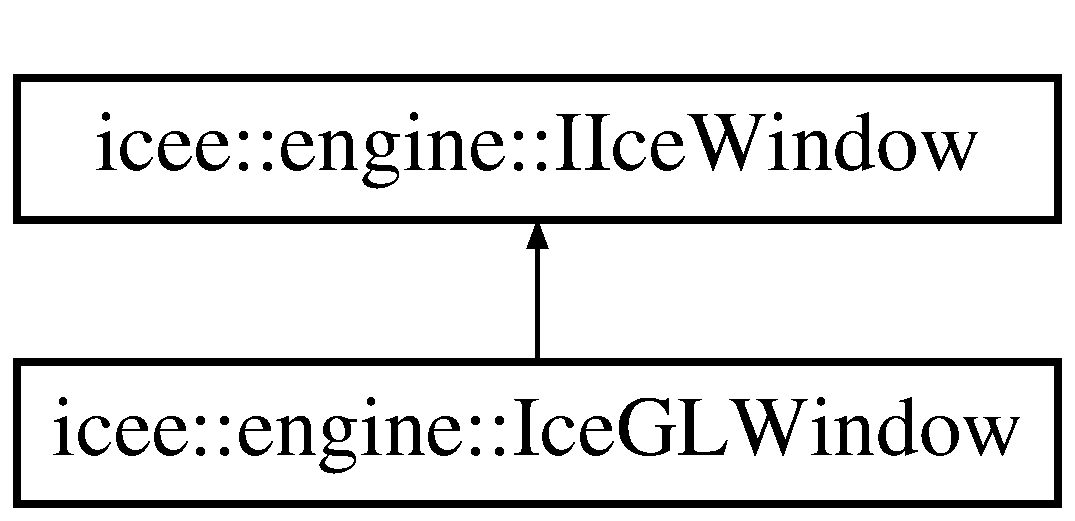
\includegraphics[height=2.000000cm]{classicee_1_1engine_1_1IIceWindow}
\end{center}
\end{figure}
\subsection*{Public Member Functions}
\begin{DoxyCompactItemize}
\item 
virtual \hyperlink{classicee_1_1engine_1_1IIceWindow_aaadd780b12a5cc13271c40ece6132266}{$\sim$IIceWindow} ()
\item 
virtual void $\ast$ \hyperlink{classicee_1_1engine_1_1IIceWindow_ae2ddf86f1599fd3d58d5f048e9daf5eb}{getWindowPointer} ()=0
\item 
virtual \hyperlink{namespacecompatibility_afc3ea6dfbdda98c9d2615b235b140a18}{sint32} \hyperlink{classicee_1_1engine_1_1IIceWindow_a5d7d7d89d028ccbef90caa600259b3e1}{initialize} ()=0
\item 
virtual void \hyperlink{classicee_1_1engine_1_1IIceWindow_a8c95b751fbd4e410390499c4e04913a7}{destroy} ()=0
\item 
virtual void \hyperlink{classicee_1_1engine_1_1IIceWindow_a5f89b1a117bdeb33d0a932e30b19caa2}{resize} (\hyperlink{namespacecompatibility_a51e8fe2956b4f39fe1fae96cec0d8393}{uint32} width, \hyperlink{namespacecompatibility_a51e8fe2956b4f39fe1fae96cec0d8393}{uint32} height)=0
\item 
virtual \hyperlink{namespacecompatibility_afc3ea6dfbdda98c9d2615b235b140a18}{sint32} \hyperlink{classicee_1_1engine_1_1IIceWindow_a48d4b1589c43d030d0d307dc36d608f3}{handleEvents} ()=0
\item 
virtual void \hyperlink{classicee_1_1engine_1_1IIceWindow_ad98b0505e03b1979e75ff1673edfa17f}{render} ()=0
\item 
virtual bool \hyperlink{classicee_1_1engine_1_1IIceWindow_afd79bc3368348b54b1c98745d206f2a5}{blah} ()=0
\item 
virtual \hyperlink{classicee_1_1engine_1_1ISceneManager}{ISceneManager} $\ast$ \hyperlink{classicee_1_1engine_1_1IIceWindow_ac67a17339f3ab2c2996de03f3bfbdf3b}{getSceneManager} ()=0
\end{DoxyCompactItemize}
\subsection*{Protected Attributes}
\begin{DoxyCompactItemize}
\item 
\hyperlink{namespacecompatibility_afc3ea6dfbdda98c9d2615b235b140a18}{sint32} \hyperlink{classicee_1_1engine_1_1IIceWindow_ad0a4dec01c6f8c8a964aa912a0051fac}{x\_\-}
\item 
\hyperlink{namespacecompatibility_afc3ea6dfbdda98c9d2615b235b140a18}{sint32} \hyperlink{classicee_1_1engine_1_1IIceWindow_a962150de24c538d079afc4f29148008b}{y\_\-}
\item 
\hyperlink{namespacecompatibility_a51e8fe2956b4f39fe1fae96cec0d8393}{uint32} \hyperlink{classicee_1_1engine_1_1IIceWindow_a87ae4186431df77c47ac5c6fc8a1c8bc}{width\_\-}
\item 
\hyperlink{namespacecompatibility_a51e8fe2956b4f39fe1fae96cec0d8393}{uint32} \hyperlink{classicee_1_1engine_1_1IIceWindow_a65267bef4575d2b16e5a8186e705e07d}{height\_\-}
\item 
\hyperlink{namespacecompatibility_a51e8fe2956b4f39fe1fae96cec0d8393}{uint32} \hyperlink{classicee_1_1engine_1_1IIceWindow_a310d4e897aa1cff48bd44ae3756e03b2}{depth\_\-}
\end{DoxyCompactItemize}


\subsection{Constructor \& Destructor Documentation}
\hypertarget{classicee_1_1engine_1_1IIceWindow_aaadd780b12a5cc13271c40ece6132266}{
\index{icee::engine::IIceWindow@{icee::engine::IIceWindow}!$\sim$IIceWindow@{$\sim$IIceWindow}}
\index{$\sim$IIceWindow@{$\sim$IIceWindow}!icee::engine::IIceWindow@{icee::engine::IIceWindow}}
\subsubsection[{$\sim$IIceWindow}]{\setlength{\rightskip}{0pt plus 5cm}virtual icee::engine::IIceWindow::$\sim$IIceWindow (
\begin{DoxyParamCaption}
{}
\end{DoxyParamCaption}
)\hspace{0.3cm}{\ttfamily  \mbox{[}inline, virtual\mbox{]}}}}
\label{classicee_1_1engine_1_1IIceWindow_aaadd780b12a5cc13271c40ece6132266}


\subsection{Member Function Documentation}
\hypertarget{classicee_1_1engine_1_1IIceWindow_afd79bc3368348b54b1c98745d206f2a5}{
\index{icee::engine::IIceWindow@{icee::engine::IIceWindow}!blah@{blah}}
\index{blah@{blah}!icee::engine::IIceWindow@{icee::engine::IIceWindow}}
\subsubsection[{blah}]{\setlength{\rightskip}{0pt plus 5cm}virtual bool icee::engine::IIceWindow::blah (
\begin{DoxyParamCaption}
{}
\end{DoxyParamCaption}
)\hspace{0.3cm}{\ttfamily  \mbox{[}pure virtual\mbox{]}}}}
\label{classicee_1_1engine_1_1IIceWindow_afd79bc3368348b54b1c98745d206f2a5}


Implemented in \hyperlink{classicee_1_1engine_1_1IceGLWindow_ab686b165d4359e0666dc2214e3d96117}{icee::engine::IceGLWindow}.

\hypertarget{classicee_1_1engine_1_1IIceWindow_a8c95b751fbd4e410390499c4e04913a7}{
\index{icee::engine::IIceWindow@{icee::engine::IIceWindow}!destroy@{destroy}}
\index{destroy@{destroy}!icee::engine::IIceWindow@{icee::engine::IIceWindow}}
\subsubsection[{destroy}]{\setlength{\rightskip}{0pt plus 5cm}virtual void icee::engine::IIceWindow::destroy (
\begin{DoxyParamCaption}
{}
\end{DoxyParamCaption}
)\hspace{0.3cm}{\ttfamily  \mbox{[}pure virtual\mbox{]}}}}
\label{classicee_1_1engine_1_1IIceWindow_a8c95b751fbd4e410390499c4e04913a7}


Implemented in \hyperlink{classicee_1_1engine_1_1IceGLWindow_ad6fa5825e2205d7f2a93da5bfd0dfbcb}{icee::engine::IceGLWindow}.

\hypertarget{classicee_1_1engine_1_1IIceWindow_ac67a17339f3ab2c2996de03f3bfbdf3b}{
\index{icee::engine::IIceWindow@{icee::engine::IIceWindow}!getSceneManager@{getSceneManager}}
\index{getSceneManager@{getSceneManager}!icee::engine::IIceWindow@{icee::engine::IIceWindow}}
\subsubsection[{getSceneManager}]{\setlength{\rightskip}{0pt plus 5cm}virtual {\bf ISceneManager}$\ast$ icee::engine::IIceWindow::getSceneManager (
\begin{DoxyParamCaption}
{}
\end{DoxyParamCaption}
)\hspace{0.3cm}{\ttfamily  \mbox{[}pure virtual\mbox{]}}}}
\label{classicee_1_1engine_1_1IIceWindow_ac67a17339f3ab2c2996de03f3bfbdf3b}


Implemented in \hyperlink{classicee_1_1engine_1_1IceGLWindow_a5b181115911d51611e2ba50fddc6f8d9}{icee::engine::IceGLWindow}.

\hypertarget{classicee_1_1engine_1_1IIceWindow_ae2ddf86f1599fd3d58d5f048e9daf5eb}{
\index{icee::engine::IIceWindow@{icee::engine::IIceWindow}!getWindowPointer@{getWindowPointer}}
\index{getWindowPointer@{getWindowPointer}!icee::engine::IIceWindow@{icee::engine::IIceWindow}}
\subsubsection[{getWindowPointer}]{\setlength{\rightskip}{0pt plus 5cm}virtual void$\ast$ icee::engine::IIceWindow::getWindowPointer (
\begin{DoxyParamCaption}
{}
\end{DoxyParamCaption}
)\hspace{0.3cm}{\ttfamily  \mbox{[}pure virtual\mbox{]}}}}
\label{classicee_1_1engine_1_1IIceWindow_ae2ddf86f1599fd3d58d5f048e9daf5eb}


Implemented in \hyperlink{classicee_1_1engine_1_1IceGLWindow_af041e4ce63d97bb82867dfc03b12c0d7}{icee::engine::IceGLWindow}.

\hypertarget{classicee_1_1engine_1_1IIceWindow_a48d4b1589c43d030d0d307dc36d608f3}{
\index{icee::engine::IIceWindow@{icee::engine::IIceWindow}!handleEvents@{handleEvents}}
\index{handleEvents@{handleEvents}!icee::engine::IIceWindow@{icee::engine::IIceWindow}}
\subsubsection[{handleEvents}]{\setlength{\rightskip}{0pt plus 5cm}virtual {\bf sint32} icee::engine::IIceWindow::handleEvents (
\begin{DoxyParamCaption}
{}
\end{DoxyParamCaption}
)\hspace{0.3cm}{\ttfamily  \mbox{[}pure virtual\mbox{]}}}}
\label{classicee_1_1engine_1_1IIceWindow_a48d4b1589c43d030d0d307dc36d608f3}


Implemented in \hyperlink{classicee_1_1engine_1_1IceGLWindow_a6b1aa21ff2b90a665647df912166d33a}{icee::engine::IceGLWindow}.

\hypertarget{classicee_1_1engine_1_1IIceWindow_a5d7d7d89d028ccbef90caa600259b3e1}{
\index{icee::engine::IIceWindow@{icee::engine::IIceWindow}!initialize@{initialize}}
\index{initialize@{initialize}!icee::engine::IIceWindow@{icee::engine::IIceWindow}}
\subsubsection[{initialize}]{\setlength{\rightskip}{0pt plus 5cm}virtual {\bf sint32} icee::engine::IIceWindow::initialize (
\begin{DoxyParamCaption}
{}
\end{DoxyParamCaption}
)\hspace{0.3cm}{\ttfamily  \mbox{[}pure virtual\mbox{]}}}}
\label{classicee_1_1engine_1_1IIceWindow_a5d7d7d89d028ccbef90caa600259b3e1}


Implemented in \hyperlink{classicee_1_1engine_1_1IceGLWindow_a58bbfb06402448f1e7791d699ce084b3}{icee::engine::IceGLWindow}.

\hypertarget{classicee_1_1engine_1_1IIceWindow_ad98b0505e03b1979e75ff1673edfa17f}{
\index{icee::engine::IIceWindow@{icee::engine::IIceWindow}!render@{render}}
\index{render@{render}!icee::engine::IIceWindow@{icee::engine::IIceWindow}}
\subsubsection[{render}]{\setlength{\rightskip}{0pt plus 5cm}virtual void icee::engine::IIceWindow::render (
\begin{DoxyParamCaption}
{}
\end{DoxyParamCaption}
)\hspace{0.3cm}{\ttfamily  \mbox{[}pure virtual\mbox{]}}}}
\label{classicee_1_1engine_1_1IIceWindow_ad98b0505e03b1979e75ff1673edfa17f}


Implemented in \hyperlink{classicee_1_1engine_1_1IceGLWindow_a766acd9860c1d9160706f168105e72a5}{icee::engine::IceGLWindow}.

\hypertarget{classicee_1_1engine_1_1IIceWindow_a5f89b1a117bdeb33d0a932e30b19caa2}{
\index{icee::engine::IIceWindow@{icee::engine::IIceWindow}!resize@{resize}}
\index{resize@{resize}!icee::engine::IIceWindow@{icee::engine::IIceWindow}}
\subsubsection[{resize}]{\setlength{\rightskip}{0pt plus 5cm}virtual void icee::engine::IIceWindow::resize (
\begin{DoxyParamCaption}
\item[{{\bf uint32}}]{width, }
\item[{{\bf uint32}}]{height}
\end{DoxyParamCaption}
)\hspace{0.3cm}{\ttfamily  \mbox{[}pure virtual\mbox{]}}}}
\label{classicee_1_1engine_1_1IIceWindow_a5f89b1a117bdeb33d0a932e30b19caa2}


Implemented in \hyperlink{classicee_1_1engine_1_1IceGLWindow_a130ecba0ab9ae8d73e86726232be532a}{icee::engine::IceGLWindow}.



\subsection{Member Data Documentation}
\hypertarget{classicee_1_1engine_1_1IIceWindow_a310d4e897aa1cff48bd44ae3756e03b2}{
\index{icee::engine::IIceWindow@{icee::engine::IIceWindow}!depth\_\-@{depth\_\-}}
\index{depth\_\-@{depth\_\-}!icee::engine::IIceWindow@{icee::engine::IIceWindow}}
\subsubsection[{depth\_\-}]{\setlength{\rightskip}{0pt plus 5cm}{\bf uint32} {\bf icee::engine::IIceWindow::depth\_\-}\hspace{0.3cm}{\ttfamily  \mbox{[}protected\mbox{]}}}}
\label{classicee_1_1engine_1_1IIceWindow_a310d4e897aa1cff48bd44ae3756e03b2}
\hypertarget{classicee_1_1engine_1_1IIceWindow_a65267bef4575d2b16e5a8186e705e07d}{
\index{icee::engine::IIceWindow@{icee::engine::IIceWindow}!height\_\-@{height\_\-}}
\index{height\_\-@{height\_\-}!icee::engine::IIceWindow@{icee::engine::IIceWindow}}
\subsubsection[{height\_\-}]{\setlength{\rightskip}{0pt plus 5cm}{\bf uint32} {\bf icee::engine::IIceWindow::height\_\-}\hspace{0.3cm}{\ttfamily  \mbox{[}protected\mbox{]}}}}
\label{classicee_1_1engine_1_1IIceWindow_a65267bef4575d2b16e5a8186e705e07d}
\hypertarget{classicee_1_1engine_1_1IIceWindow_a87ae4186431df77c47ac5c6fc8a1c8bc}{
\index{icee::engine::IIceWindow@{icee::engine::IIceWindow}!width\_\-@{width\_\-}}
\index{width\_\-@{width\_\-}!icee::engine::IIceWindow@{icee::engine::IIceWindow}}
\subsubsection[{width\_\-}]{\setlength{\rightskip}{0pt plus 5cm}{\bf uint32} {\bf icee::engine::IIceWindow::width\_\-}\hspace{0.3cm}{\ttfamily  \mbox{[}protected\mbox{]}}}}
\label{classicee_1_1engine_1_1IIceWindow_a87ae4186431df77c47ac5c6fc8a1c8bc}
\hypertarget{classicee_1_1engine_1_1IIceWindow_ad0a4dec01c6f8c8a964aa912a0051fac}{
\index{icee::engine::IIceWindow@{icee::engine::IIceWindow}!x\_\-@{x\_\-}}
\index{x\_\-@{x\_\-}!icee::engine::IIceWindow@{icee::engine::IIceWindow}}
\subsubsection[{x\_\-}]{\setlength{\rightskip}{0pt plus 5cm}{\bf sint32} {\bf icee::engine::IIceWindow::x\_\-}\hspace{0.3cm}{\ttfamily  \mbox{[}protected\mbox{]}}}}
\label{classicee_1_1engine_1_1IIceWindow_ad0a4dec01c6f8c8a964aa912a0051fac}
\hypertarget{classicee_1_1engine_1_1IIceWindow_a962150de24c538d079afc4f29148008b}{
\index{icee::engine::IIceWindow@{icee::engine::IIceWindow}!y\_\-@{y\_\-}}
\index{y\_\-@{y\_\-}!icee::engine::IIceWindow@{icee::engine::IIceWindow}}
\subsubsection[{y\_\-}]{\setlength{\rightskip}{0pt plus 5cm}{\bf sint32} {\bf icee::engine::IIceWindow::y\_\-}\hspace{0.3cm}{\ttfamily  \mbox{[}protected\mbox{]}}}}
\label{classicee_1_1engine_1_1IIceWindow_a962150de24c538d079afc4f29148008b}


The documentation for this class was generated from the following file:\begin{DoxyCompactItemize}
\item 
src/engine/\hyperlink{IIceWindow_8h}{IIceWindow.h}\end{DoxyCompactItemize}

\hypertarget{classicee_1_1engine_1_1IMesh}{
\section{icee::engine::IMesh Class Reference}
\label{classicee_1_1engine_1_1IMesh}\index{icee::engine::IMesh@{icee::engine::IMesh}}
}


{\ttfamily \#include $<$IMesh.h$>$}

\subsection*{Public Member Functions}
\begin{DoxyCompactItemize}
\item 
\hyperlink{classicee_1_1engine_1_1IMesh_a2c997918ab61669e3790b09c17d2fd99}{IMesh} ()
\item 
virtual \hyperlink{classicee_1_1engine_1_1IMesh_abfe38508bbe3f0604f083f3be96ee240}{$\sim$IMesh} ()
\end{DoxyCompactItemize}


\subsection{Constructor \& Destructor Documentation}
\hypertarget{classicee_1_1engine_1_1IMesh_a2c997918ab61669e3790b09c17d2fd99}{
\index{icee::engine::IMesh@{icee::engine::IMesh}!IMesh@{IMesh}}
\index{IMesh@{IMesh}!icee::engine::IMesh@{icee::engine::IMesh}}
\subsubsection[{IMesh}]{\setlength{\rightskip}{0pt plus 5cm}icee::engine::IMesh::IMesh (
\begin{DoxyParamCaption}
{}
\end{DoxyParamCaption}
)}}
\label{classicee_1_1engine_1_1IMesh_a2c997918ab61669e3790b09c17d2fd99}
\hypertarget{classicee_1_1engine_1_1IMesh_abfe38508bbe3f0604f083f3be96ee240}{
\index{icee::engine::IMesh@{icee::engine::IMesh}!$\sim$IMesh@{$\sim$IMesh}}
\index{$\sim$IMesh@{$\sim$IMesh}!icee::engine::IMesh@{icee::engine::IMesh}}
\subsubsection[{$\sim$IMesh}]{\setlength{\rightskip}{0pt plus 5cm}virtual icee::engine::IMesh::$\sim$IMesh (
\begin{DoxyParamCaption}
{}
\end{DoxyParamCaption}
)\hspace{0.3cm}{\ttfamily  \mbox{[}virtual\mbox{]}}}}
\label{classicee_1_1engine_1_1IMesh_abfe38508bbe3f0604f083f3be96ee240}


The documentation for this class was generated from the following file:\begin{DoxyCompactItemize}
\item 
src/engine/\hyperlink{IMesh_8h}{IMesh.h}\end{DoxyCompactItemize}

\hypertarget{classicee_1_1engine_1_1IOS}{
\section{icee::engine::IOS Class Reference}
\label{classicee_1_1engine_1_1IOS}\index{icee::engine::IOS@{icee::engine::IOS}}
}


{\ttfamily \#include $<$IOS.h$>$}

Inheritance diagram for icee::engine::IOS:\begin{figure}[H]
\begin{center}
\leavevmode
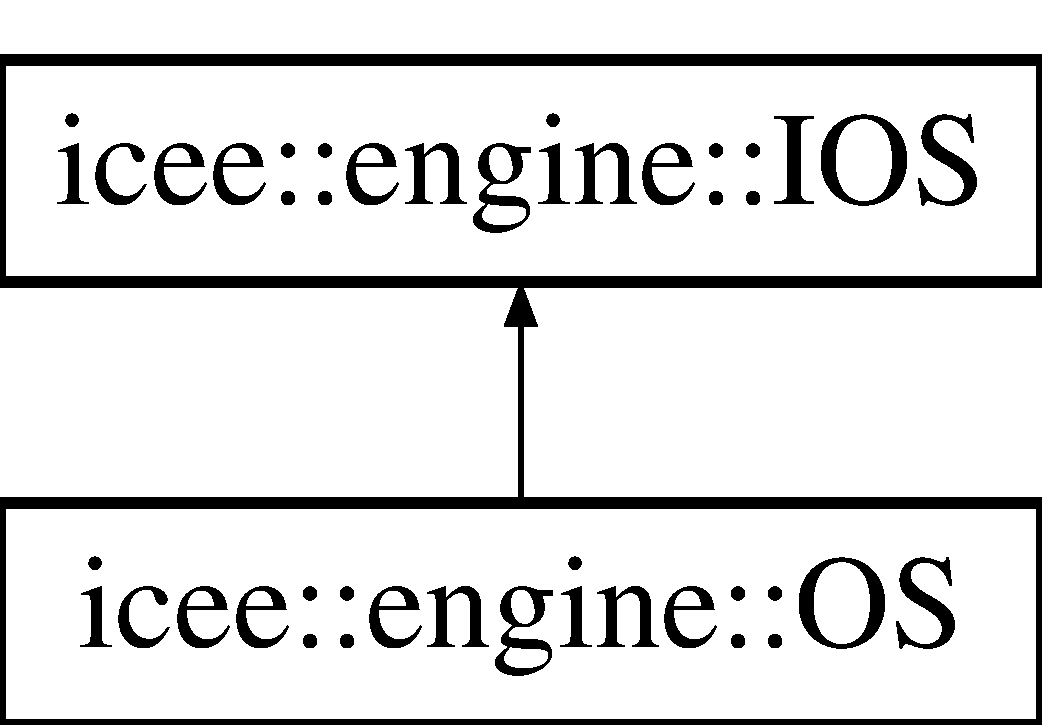
\includegraphics[height=2.000000cm]{classicee_1_1engine_1_1IOS}
\end{center}
\end{figure}
\subsection*{Public Member Functions}
\begin{DoxyCompactItemize}
\item 
virtual \hyperlink{classicee_1_1engine_1_1IOS_a6ab257b860563730ade56a7911fa9ea1}{$\sim$IOS} ()
\item 
virtual \hyperlink{namespacecompatibility_afc3ea6dfbdda98c9d2615b235b140a18}{sint32} \hyperlink{classicee_1_1engine_1_1IOS_aac944785a1b436e75b9f22881836ae75}{initialize} ()=0
\item 
virtual \hyperlink{classicee_1_1engine_1_1IIceWindow}{IIceWindow} $\ast$ \hyperlink{classicee_1_1engine_1_1IOS_a45a2101e58e5eb66774e717b26a343bb}{createWindow} (\hyperlink{namespacecompatibility_a51e8fe2956b4f39fe1fae96cec0d8393}{uint32} width=800, \hyperlink{namespacecompatibility_a51e8fe2956b4f39fe1fae96cec0d8393}{uint32} height=600, \hyperlink{namespacecompatibility_a51e8fe2956b4f39fe1fae96cec0d8393}{uint32} depth=24, bool fullscreen=false, bool vsync=false)=0
\end{DoxyCompactItemize}


\subsection{Constructor \& Destructor Documentation}
\hypertarget{classicee_1_1engine_1_1IOS_a6ab257b860563730ade56a7911fa9ea1}{
\index{icee::engine::IOS@{icee::engine::IOS}!$\sim$IOS@{$\sim$IOS}}
\index{$\sim$IOS@{$\sim$IOS}!icee::engine::IOS@{icee::engine::IOS}}
\subsubsection[{$\sim$IOS}]{\setlength{\rightskip}{0pt plus 5cm}virtual icee::engine::IOS::$\sim$IOS (
\begin{DoxyParamCaption}
{}
\end{DoxyParamCaption}
)\hspace{0.3cm}{\ttfamily  \mbox{[}inline, virtual\mbox{]}}}}
\label{classicee_1_1engine_1_1IOS_a6ab257b860563730ade56a7911fa9ea1}


\subsection{Member Function Documentation}
\hypertarget{classicee_1_1engine_1_1IOS_a45a2101e58e5eb66774e717b26a343bb}{
\index{icee::engine::IOS@{icee::engine::IOS}!createWindow@{createWindow}}
\index{createWindow@{createWindow}!icee::engine::IOS@{icee::engine::IOS}}
\subsubsection[{createWindow}]{\setlength{\rightskip}{0pt plus 5cm}virtual {\bf IIceWindow}$\ast$ icee::engine::IOS::createWindow (
\begin{DoxyParamCaption}
\item[{{\bf uint32}}]{width = {\ttfamily 800}, }
\item[{{\bf uint32}}]{height = {\ttfamily 600}, }
\item[{{\bf uint32}}]{depth = {\ttfamily 24}, }
\item[{bool}]{fullscreen = {\ttfamily false}, }
\item[{bool}]{vsync = {\ttfamily false}}
\end{DoxyParamCaption}
)\hspace{0.3cm}{\ttfamily  \mbox{[}pure virtual\mbox{]}}}}
\label{classicee_1_1engine_1_1IOS_a45a2101e58e5eb66774e717b26a343bb}


Implemented in \hyperlink{classicee_1_1engine_1_1OS_a460645e9a18535546cecb2280cfe364e}{icee::engine::OS}.

\hypertarget{classicee_1_1engine_1_1IOS_aac944785a1b436e75b9f22881836ae75}{
\index{icee::engine::IOS@{icee::engine::IOS}!initialize@{initialize}}
\index{initialize@{initialize}!icee::engine::IOS@{icee::engine::IOS}}
\subsubsection[{initialize}]{\setlength{\rightskip}{0pt plus 5cm}virtual {\bf sint32} icee::engine::IOS::initialize (
\begin{DoxyParamCaption}
{}
\end{DoxyParamCaption}
)\hspace{0.3cm}{\ttfamily  \mbox{[}pure virtual\mbox{]}}}}
\label{classicee_1_1engine_1_1IOS_aac944785a1b436e75b9f22881836ae75}


Implemented in \hyperlink{classicee_1_1engine_1_1OS_a42869381836268f3c27d610e43743da3}{icee::engine::OS}.



The documentation for this class was generated from the following file:\begin{DoxyCompactItemize}
\item 
src/engine/\hyperlink{IOS_8h}{IOS.h}\end{DoxyCompactItemize}

\hypertarget{classicee_1_1engine_1_1ISceneManager}{
\section{icee::engine::ISceneManager Class Reference}
\label{classicee_1_1engine_1_1ISceneManager}\index{icee::engine::ISceneManager@{icee::engine::ISceneManager}}
}


{\ttfamily \#include $<$ISceneManager.h$>$}

Inheritance diagram for icee::engine::ISceneManager:\begin{figure}[H]
\begin{center}
\leavevmode
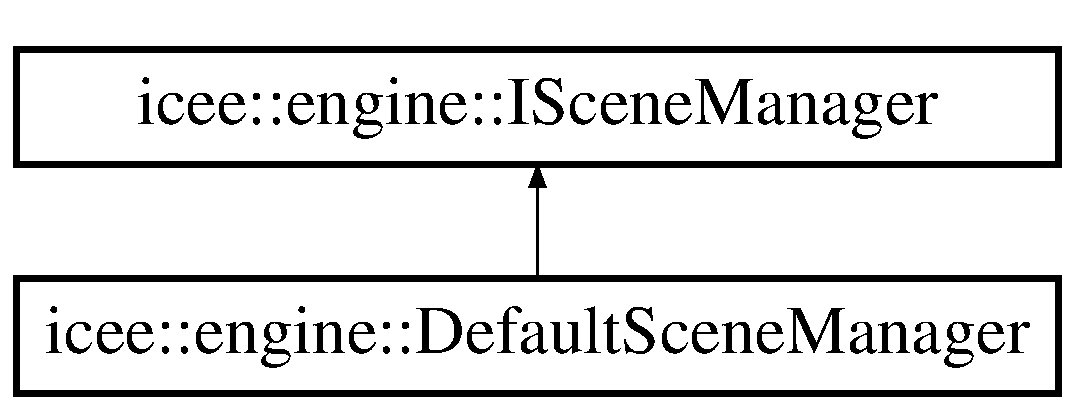
\includegraphics[height=2.000000cm]{classicee_1_1engine_1_1ISceneManager}
\end{center}
\end{figure}
\subsection*{Public Member Functions}
\begin{DoxyCompactItemize}
\item 
virtual \hyperlink{classicee_1_1engine_1_1ISceneManager_a0ce0427b8cfac77f1e520a5da7169a88}{$\sim$ISceneManager} ()
\item 
virtual \hyperlink{classicee_1_1engine_1_1ISceneNode}{ISceneNode} $\ast$ \hyperlink{classicee_1_1engine_1_1ISceneManager_afc84d5f887e850807ee36732b13c3798}{addDefaultSceneNode} (const char $\ast$name, \hyperlink{classicee_1_1engine_1_1ISceneNode}{ISceneNode} $\ast$parent=0, \hyperlink{namespacecompatibility_afc3ea6dfbdda98c9d2615b235b140a18}{sint32} id=-\/1)=0
\item 
virtual \hyperlink{classicee_1_1engine_1_1ISceneNode}{ISceneNode} $\ast$ \hyperlink{classicee_1_1engine_1_1ISceneManager_aecda2ddc8edc12f6bcf63575d988f0f1}{addSceneNode} (const char $\ast$name, \hyperlink{classicee_1_1engine_1_1ISceneNode}{ISceneNode} $\ast$parent=0, \hyperlink{namespacecompatibility_afc3ea6dfbdda98c9d2615b235b140a18}{sint32} id=-\/1)=0
\item 
virtual \hyperlink{classicee_1_1engine_1_1ICameraSceneNode}{ICameraSceneNode} $\ast$ \hyperlink{classicee_1_1engine_1_1ISceneManager_a2f43eae86d27ee9fd4d8964c7073cc9b}{addCamera} (\hyperlink{classvmath_1_1Vector3f}{vmath::Vector3f} position, \hyperlink{classvmath_1_1Vector3f}{vmath::Vector3f} lookAt)=0
\item 
virtual \hyperlink{classicee_1_1engine_1_1ICameraSceneNode}{ICameraSceneNode} $\ast$ \hyperlink{classicee_1_1engine_1_1ISceneManager_a2165f1d59e5338aa9fd89d0242a38662}{addCameraFPS} (\hyperlink{classvmath_1_1Vector3f}{vmath::Vector3f} position, \hyperlink{classvmath_1_1Vector3f}{vmath::Vector3f} lookAt, \hyperlink{namespacecompatibility_a51e8fe2956b4f39fe1fae96cec0d8393}{uint32} speed, \hyperlink{namespacecompatibility_a51e8fe2956b4f39fe1fae96cec0d8393}{uint32} rotationSpeed)=0
\item 
virtual void \hyperlink{classicee_1_1engine_1_1ISceneManager_a39930cf34881d0d014b41190dd356def}{drawAll} ()=0
\end{DoxyCompactItemize}
\subsection*{Protected Attributes}
\begin{DoxyCompactItemize}
\item 
std::vector$<$ \hyperlink{classicee_1_1engine_1_1ISceneNode}{ISceneNode} $\ast$ $>$ \hyperlink{classicee_1_1engine_1_1ISceneManager_abe2884dbf5f8bb733e4eabcc92922963}{sceneNodes\_\-}
\end{DoxyCompactItemize}


\subsection{Constructor \& Destructor Documentation}
\hypertarget{classicee_1_1engine_1_1ISceneManager_a0ce0427b8cfac77f1e520a5da7169a88}{
\index{icee::engine::ISceneManager@{icee::engine::ISceneManager}!$\sim$ISceneManager@{$\sim$ISceneManager}}
\index{$\sim$ISceneManager@{$\sim$ISceneManager}!icee::engine::ISceneManager@{icee::engine::ISceneManager}}
\subsubsection[{$\sim$ISceneManager}]{\setlength{\rightskip}{0pt plus 5cm}virtual icee::engine::ISceneManager::$\sim$ISceneManager (
\begin{DoxyParamCaption}
{}
\end{DoxyParamCaption}
)\hspace{0.3cm}{\ttfamily  \mbox{[}inline, virtual\mbox{]}}}}
\label{classicee_1_1engine_1_1ISceneManager_a0ce0427b8cfac77f1e520a5da7169a88}


\subsection{Member Function Documentation}
\hypertarget{classicee_1_1engine_1_1ISceneManager_a2f43eae86d27ee9fd4d8964c7073cc9b}{
\index{icee::engine::ISceneManager@{icee::engine::ISceneManager}!addCamera@{addCamera}}
\index{addCamera@{addCamera}!icee::engine::ISceneManager@{icee::engine::ISceneManager}}
\subsubsection[{addCamera}]{\setlength{\rightskip}{0pt plus 5cm}virtual {\bf ICameraSceneNode}$\ast$ icee::engine::ISceneManager::addCamera (
\begin{DoxyParamCaption}
\item[{{\bf vmath::Vector3f}}]{position, }
\item[{{\bf vmath::Vector3f}}]{lookAt}
\end{DoxyParamCaption}
)\hspace{0.3cm}{\ttfamily  \mbox{[}pure virtual\mbox{]}}}}
\label{classicee_1_1engine_1_1ISceneManager_a2f43eae86d27ee9fd4d8964c7073cc9b}


Implemented in \hyperlink{classicee_1_1engine_1_1DefaultSceneManager_ac93bba8c1d23d86ae547020e0086c5a4}{icee::engine::DefaultSceneManager}.

\hypertarget{classicee_1_1engine_1_1ISceneManager_a2165f1d59e5338aa9fd89d0242a38662}{
\index{icee::engine::ISceneManager@{icee::engine::ISceneManager}!addCameraFPS@{addCameraFPS}}
\index{addCameraFPS@{addCameraFPS}!icee::engine::ISceneManager@{icee::engine::ISceneManager}}
\subsubsection[{addCameraFPS}]{\setlength{\rightskip}{0pt plus 5cm}virtual {\bf ICameraSceneNode}$\ast$ icee::engine::ISceneManager::addCameraFPS (
\begin{DoxyParamCaption}
\item[{{\bf vmath::Vector3f}}]{position, }
\item[{{\bf vmath::Vector3f}}]{lookAt, }
\item[{{\bf uint32}}]{speed, }
\item[{{\bf uint32}}]{rotationSpeed}
\end{DoxyParamCaption}
)\hspace{0.3cm}{\ttfamily  \mbox{[}pure virtual\mbox{]}}}}
\label{classicee_1_1engine_1_1ISceneManager_a2165f1d59e5338aa9fd89d0242a38662}


Implemented in \hyperlink{classicee_1_1engine_1_1DefaultSceneManager_a75b9d066c4ff5f231e9806cfbef64caf}{icee::engine::DefaultSceneManager}.

\hypertarget{classicee_1_1engine_1_1ISceneManager_afc84d5f887e850807ee36732b13c3798}{
\index{icee::engine::ISceneManager@{icee::engine::ISceneManager}!addDefaultSceneNode@{addDefaultSceneNode}}
\index{addDefaultSceneNode@{addDefaultSceneNode}!icee::engine::ISceneManager@{icee::engine::ISceneManager}}
\subsubsection[{addDefaultSceneNode}]{\setlength{\rightskip}{0pt plus 5cm}virtual {\bf ISceneNode}$\ast$ icee::engine::ISceneManager::addDefaultSceneNode (
\begin{DoxyParamCaption}
\item[{const char $\ast$}]{name, }
\item[{{\bf ISceneNode} $\ast$}]{parent = {\ttfamily 0}, }
\item[{{\bf sint32}}]{id = {\ttfamily -\/1}}
\end{DoxyParamCaption}
)\hspace{0.3cm}{\ttfamily  \mbox{[}pure virtual\mbox{]}}}}
\label{classicee_1_1engine_1_1ISceneManager_afc84d5f887e850807ee36732b13c3798}


Implemented in \hyperlink{classicee_1_1engine_1_1DefaultSceneManager_a92412af214e790045fb5890936ac37db}{icee::engine::DefaultSceneManager}.

\hypertarget{classicee_1_1engine_1_1ISceneManager_aecda2ddc8edc12f6bcf63575d988f0f1}{
\index{icee::engine::ISceneManager@{icee::engine::ISceneManager}!addSceneNode@{addSceneNode}}
\index{addSceneNode@{addSceneNode}!icee::engine::ISceneManager@{icee::engine::ISceneManager}}
\subsubsection[{addSceneNode}]{\setlength{\rightskip}{0pt plus 5cm}virtual {\bf ISceneNode}$\ast$ icee::engine::ISceneManager::addSceneNode (
\begin{DoxyParamCaption}
\item[{const char $\ast$}]{name, }
\item[{{\bf ISceneNode} $\ast$}]{parent = {\ttfamily 0}, }
\item[{{\bf sint32}}]{id = {\ttfamily -\/1}}
\end{DoxyParamCaption}
)\hspace{0.3cm}{\ttfamily  \mbox{[}pure virtual\mbox{]}}}}
\label{classicee_1_1engine_1_1ISceneManager_aecda2ddc8edc12f6bcf63575d988f0f1}


Implemented in \hyperlink{classicee_1_1engine_1_1DefaultSceneManager_a8e19127f7542d263d8b9b34c170f40fd}{icee::engine::DefaultSceneManager}.

\hypertarget{classicee_1_1engine_1_1ISceneManager_a39930cf34881d0d014b41190dd356def}{
\index{icee::engine::ISceneManager@{icee::engine::ISceneManager}!drawAll@{drawAll}}
\index{drawAll@{drawAll}!icee::engine::ISceneManager@{icee::engine::ISceneManager}}
\subsubsection[{drawAll}]{\setlength{\rightskip}{0pt plus 5cm}virtual void icee::engine::ISceneManager::drawAll (
\begin{DoxyParamCaption}
{}
\end{DoxyParamCaption}
)\hspace{0.3cm}{\ttfamily  \mbox{[}pure virtual\mbox{]}}}}
\label{classicee_1_1engine_1_1ISceneManager_a39930cf34881d0d014b41190dd356def}


Implemented in \hyperlink{classicee_1_1engine_1_1DefaultSceneManager_add821d9d71b613663c391cbc37fe5f0f}{icee::engine::DefaultSceneManager}.



\subsection{Member Data Documentation}
\hypertarget{classicee_1_1engine_1_1ISceneManager_abe2884dbf5f8bb733e4eabcc92922963}{
\index{icee::engine::ISceneManager@{icee::engine::ISceneManager}!sceneNodes\_\-@{sceneNodes\_\-}}
\index{sceneNodes\_\-@{sceneNodes\_\-}!icee::engine::ISceneManager@{icee::engine::ISceneManager}}
\subsubsection[{sceneNodes\_\-}]{\setlength{\rightskip}{0pt plus 5cm}std::vector$<${\bf ISceneNode}$\ast$$>$ {\bf icee::engine::ISceneManager::sceneNodes\_\-}\hspace{0.3cm}{\ttfamily  \mbox{[}protected\mbox{]}}}}
\label{classicee_1_1engine_1_1ISceneManager_abe2884dbf5f8bb733e4eabcc92922963}


The documentation for this class was generated from the following file:\begin{DoxyCompactItemize}
\item 
src/engine/\hyperlink{ISceneManager_8h}{ISceneManager.h}\end{DoxyCompactItemize}

\hypertarget{classicee_1_1engine_1_1ISceneNode}{
\section{icee::engine::ISceneNode Class Reference}
\label{classicee_1_1engine_1_1ISceneNode}\index{icee::engine::ISceneNode@{icee::engine::ISceneNode}}
}


{\ttfamily \#include $<$ISceneNode.h$>$}

Inheritance diagram for icee::engine::ISceneNode:\begin{figure}[H]
\begin{center}
\leavevmode
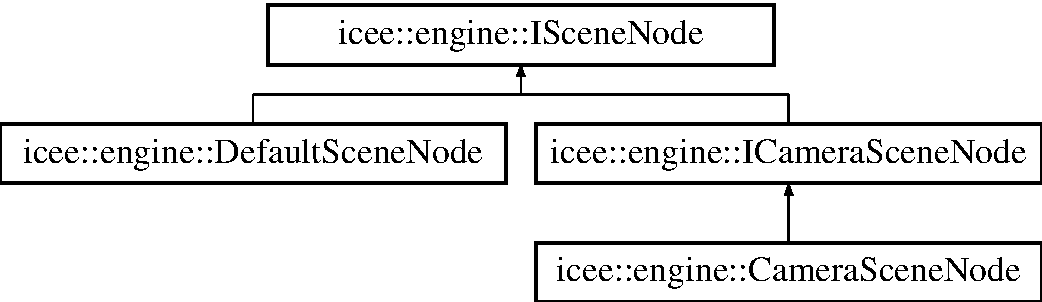
\includegraphics[height=3.000000cm]{classicee_1_1engine_1_1ISceneNode}
\end{center}
\end{figure}
\subsection*{Public Member Functions}
\begin{DoxyCompactItemize}
\item 
\hyperlink{classicee_1_1engine_1_1ISceneNode_a1a32b1c88daaa734b44e179e6685f725}{ISceneNode} ()
\item 
virtual \hyperlink{classicee_1_1engine_1_1ISceneNode_af0d0996364a4584550a882fe2e07d9e9}{$\sim$ISceneNode} ()
\item 
const \hyperlink{classvmath_1_1Vector3f}{vmath::Vector3f} \& \hyperlink{classicee_1_1engine_1_1ISceneNode_a257d4106f3e33aa74fcee8324296052d}{getPosition} () const 
\item 
void \hyperlink{classicee_1_1engine_1_1ISceneNode_a077bc5f74cea7bb0f799af977cb6361b}{setPosition} (const \hyperlink{classvmath_1_1Vector3f}{vmath::Vector3f} \&newPos)
\item 
const \hyperlink{classicee_1_1engine_1_1ISceneNode}{ISceneNode} $\ast$ \hyperlink{classicee_1_1engine_1_1ISceneNode_a8b50dcdb52ff0175fa5abf856ee8308e}{getParent} () const 
\item 
const bool \hyperlink{classicee_1_1engine_1_1ISceneNode_a07575cfd84c5dd0de037847396ad02d3}{isActive} () const 
\item 
virtual void \hyperlink{classicee_1_1engine_1_1ISceneNode_a2951ecb91b29bcc74d992de4880daa0f}{render} ()=0
\end{DoxyCompactItemize}
\subsection*{Public Attributes}
\begin{DoxyCompactItemize}
\item 
std::vector$<$ \hyperlink{namespacecompatibility_a32a2d006ac2172c0f859370287f0104c}{float32} $>$ \hyperlink{classicee_1_1engine_1_1ISceneNode_ae3d0e1a251ee6ee09557f6cf7998c738}{vertices}
\end{DoxyCompactItemize}
\subsection*{Protected Attributes}
\begin{DoxyCompactItemize}
\item 
\hyperlink{classicee_1_1engine_1_1ISceneNode}{ISceneNode} $\ast$ \hyperlink{classicee_1_1engine_1_1ISceneNode_af44b6ffb978e0fa6bc2f56bfdcdb1baa}{parent\_\-}
\item 
std::vector$<$ \hyperlink{classicee_1_1engine_1_1ISceneNode}{ISceneNode} $\ast$ $>$ \hyperlink{classicee_1_1engine_1_1ISceneNode_a1e95d624bebefac960815a8b32f13be4}{children\_\-}
\item 
\hyperlink{classvmath_1_1Vector3f}{vmath::Vector3f} \hyperlink{classicee_1_1engine_1_1ISceneNode_a6aa82e2a759e759edb3273d129fdb222}{pos\_\-}
\item 
bool \hyperlink{classicee_1_1engine_1_1ISceneNode_a619f3bd863e568a21fd487a2e98fd0fe}{active\_\-}
\end{DoxyCompactItemize}


\subsection{Constructor \& Destructor Documentation}
\hypertarget{classicee_1_1engine_1_1ISceneNode_a1a32b1c88daaa734b44e179e6685f725}{
\index{icee::engine::ISceneNode@{icee::engine::ISceneNode}!ISceneNode@{ISceneNode}}
\index{ISceneNode@{ISceneNode}!icee::engine::ISceneNode@{icee::engine::ISceneNode}}
\subsubsection[{ISceneNode}]{\setlength{\rightskip}{0pt plus 5cm}icee::engine::ISceneNode::ISceneNode (
\begin{DoxyParamCaption}
{}
\end{DoxyParamCaption}
)\hspace{0.3cm}{\ttfamily  \mbox{[}inline\mbox{]}}}}
\label{classicee_1_1engine_1_1ISceneNode_a1a32b1c88daaa734b44e179e6685f725}
\hypertarget{classicee_1_1engine_1_1ISceneNode_af0d0996364a4584550a882fe2e07d9e9}{
\index{icee::engine::ISceneNode@{icee::engine::ISceneNode}!$\sim$ISceneNode@{$\sim$ISceneNode}}
\index{$\sim$ISceneNode@{$\sim$ISceneNode}!icee::engine::ISceneNode@{icee::engine::ISceneNode}}
\subsubsection[{$\sim$ISceneNode}]{\setlength{\rightskip}{0pt plus 5cm}virtual icee::engine::ISceneNode::$\sim$ISceneNode (
\begin{DoxyParamCaption}
{}
\end{DoxyParamCaption}
)\hspace{0.3cm}{\ttfamily  \mbox{[}inline, virtual\mbox{]}}}}
\label{classicee_1_1engine_1_1ISceneNode_af0d0996364a4584550a882fe2e07d9e9}


\subsection{Member Function Documentation}
\hypertarget{classicee_1_1engine_1_1ISceneNode_a8b50dcdb52ff0175fa5abf856ee8308e}{
\index{icee::engine::ISceneNode@{icee::engine::ISceneNode}!getParent@{getParent}}
\index{getParent@{getParent}!icee::engine::ISceneNode@{icee::engine::ISceneNode}}
\subsubsection[{getParent}]{\setlength{\rightskip}{0pt plus 5cm}const {\bf ISceneNode}$\ast$ icee::engine::ISceneNode::getParent (
\begin{DoxyParamCaption}
{}
\end{DoxyParamCaption}
) const\hspace{0.3cm}{\ttfamily  \mbox{[}inline\mbox{]}}}}
\label{classicee_1_1engine_1_1ISceneNode_a8b50dcdb52ff0175fa5abf856ee8308e}
\hypertarget{classicee_1_1engine_1_1ISceneNode_a257d4106f3e33aa74fcee8324296052d}{
\index{icee::engine::ISceneNode@{icee::engine::ISceneNode}!getPosition@{getPosition}}
\index{getPosition@{getPosition}!icee::engine::ISceneNode@{icee::engine::ISceneNode}}
\subsubsection[{getPosition}]{\setlength{\rightskip}{0pt plus 5cm}const {\bf vmath::Vector3f}\& icee::engine::ISceneNode::getPosition (
\begin{DoxyParamCaption}
{}
\end{DoxyParamCaption}
) const\hspace{0.3cm}{\ttfamily  \mbox{[}inline\mbox{]}}}}
\label{classicee_1_1engine_1_1ISceneNode_a257d4106f3e33aa74fcee8324296052d}
\hypertarget{classicee_1_1engine_1_1ISceneNode_a07575cfd84c5dd0de037847396ad02d3}{
\index{icee::engine::ISceneNode@{icee::engine::ISceneNode}!isActive@{isActive}}
\index{isActive@{isActive}!icee::engine::ISceneNode@{icee::engine::ISceneNode}}
\subsubsection[{isActive}]{\setlength{\rightskip}{0pt plus 5cm}const bool icee::engine::ISceneNode::isActive (
\begin{DoxyParamCaption}
{}
\end{DoxyParamCaption}
) const\hspace{0.3cm}{\ttfamily  \mbox{[}inline\mbox{]}}}}
\label{classicee_1_1engine_1_1ISceneNode_a07575cfd84c5dd0de037847396ad02d3}
\hypertarget{classicee_1_1engine_1_1ISceneNode_a2951ecb91b29bcc74d992de4880daa0f}{
\index{icee::engine::ISceneNode@{icee::engine::ISceneNode}!render@{render}}
\index{render@{render}!icee::engine::ISceneNode@{icee::engine::ISceneNode}}
\subsubsection[{render}]{\setlength{\rightskip}{0pt plus 5cm}virtual void icee::engine::ISceneNode::render (
\begin{DoxyParamCaption}
{}
\end{DoxyParamCaption}
)\hspace{0.3cm}{\ttfamily  \mbox{[}pure virtual\mbox{]}}}}
\label{classicee_1_1engine_1_1ISceneNode_a2951ecb91b29bcc74d992de4880daa0f}


Implemented in \hyperlink{classicee_1_1engine_1_1CameraSceneNode_a230b6af4d2c61341e7146e901c25e8be}{icee::engine::CameraSceneNode}, \hyperlink{classicee_1_1engine_1_1DefaultSceneNode_aed9092adb48382ec5423f7d2224d8fef}{icee::engine::DefaultSceneNode}, and \hyperlink{classicee_1_1engine_1_1ICameraSceneNode_af4996793cf1cc2d0ccdf541e94ac9609}{icee::engine::ICameraSceneNode}.

\hypertarget{classicee_1_1engine_1_1ISceneNode_a077bc5f74cea7bb0f799af977cb6361b}{
\index{icee::engine::ISceneNode@{icee::engine::ISceneNode}!setPosition@{setPosition}}
\index{setPosition@{setPosition}!icee::engine::ISceneNode@{icee::engine::ISceneNode}}
\subsubsection[{setPosition}]{\setlength{\rightskip}{0pt plus 5cm}void icee::engine::ISceneNode::setPosition (
\begin{DoxyParamCaption}
\item[{const {\bf vmath::Vector3f} \&}]{newPos}
\end{DoxyParamCaption}
)\hspace{0.3cm}{\ttfamily  \mbox{[}inline\mbox{]}}}}
\label{classicee_1_1engine_1_1ISceneNode_a077bc5f74cea7bb0f799af977cb6361b}


\subsection{Member Data Documentation}
\hypertarget{classicee_1_1engine_1_1ISceneNode_a619f3bd863e568a21fd487a2e98fd0fe}{
\index{icee::engine::ISceneNode@{icee::engine::ISceneNode}!active\_\-@{active\_\-}}
\index{active\_\-@{active\_\-}!icee::engine::ISceneNode@{icee::engine::ISceneNode}}
\subsubsection[{active\_\-}]{\setlength{\rightskip}{0pt plus 5cm}bool {\bf icee::engine::ISceneNode::active\_\-}\hspace{0.3cm}{\ttfamily  \mbox{[}protected\mbox{]}}}}
\label{classicee_1_1engine_1_1ISceneNode_a619f3bd863e568a21fd487a2e98fd0fe}
\hypertarget{classicee_1_1engine_1_1ISceneNode_a1e95d624bebefac960815a8b32f13be4}{
\index{icee::engine::ISceneNode@{icee::engine::ISceneNode}!children\_\-@{children\_\-}}
\index{children\_\-@{children\_\-}!icee::engine::ISceneNode@{icee::engine::ISceneNode}}
\subsubsection[{children\_\-}]{\setlength{\rightskip}{0pt plus 5cm}std::vector$<${\bf ISceneNode}$\ast$$>$ {\bf icee::engine::ISceneNode::children\_\-}\hspace{0.3cm}{\ttfamily  \mbox{[}protected\mbox{]}}}}
\label{classicee_1_1engine_1_1ISceneNode_a1e95d624bebefac960815a8b32f13be4}
\hypertarget{classicee_1_1engine_1_1ISceneNode_af44b6ffb978e0fa6bc2f56bfdcdb1baa}{
\index{icee::engine::ISceneNode@{icee::engine::ISceneNode}!parent\_\-@{parent\_\-}}
\index{parent\_\-@{parent\_\-}!icee::engine::ISceneNode@{icee::engine::ISceneNode}}
\subsubsection[{parent\_\-}]{\setlength{\rightskip}{0pt plus 5cm}{\bf ISceneNode}$\ast$ {\bf icee::engine::ISceneNode::parent\_\-}\hspace{0.3cm}{\ttfamily  \mbox{[}protected\mbox{]}}}}
\label{classicee_1_1engine_1_1ISceneNode_af44b6ffb978e0fa6bc2f56bfdcdb1baa}
\hypertarget{classicee_1_1engine_1_1ISceneNode_a6aa82e2a759e759edb3273d129fdb222}{
\index{icee::engine::ISceneNode@{icee::engine::ISceneNode}!pos\_\-@{pos\_\-}}
\index{pos\_\-@{pos\_\-}!icee::engine::ISceneNode@{icee::engine::ISceneNode}}
\subsubsection[{pos\_\-}]{\setlength{\rightskip}{0pt plus 5cm}{\bf vmath::Vector3f} {\bf icee::engine::ISceneNode::pos\_\-}\hspace{0.3cm}{\ttfamily  \mbox{[}protected\mbox{]}}}}
\label{classicee_1_1engine_1_1ISceneNode_a6aa82e2a759e759edb3273d129fdb222}
\hypertarget{classicee_1_1engine_1_1ISceneNode_ae3d0e1a251ee6ee09557f6cf7998c738}{
\index{icee::engine::ISceneNode@{icee::engine::ISceneNode}!vertices@{vertices}}
\index{vertices@{vertices}!icee::engine::ISceneNode@{icee::engine::ISceneNode}}
\subsubsection[{vertices}]{\setlength{\rightskip}{0pt plus 5cm}std::vector$<${\bf float32}$>$ {\bf icee::engine::ISceneNode::vertices}}}
\label{classicee_1_1engine_1_1ISceneNode_ae3d0e1a251ee6ee09557f6cf7998c738}


The documentation for this class was generated from the following file:\begin{DoxyCompactItemize}
\item 
src/engine/\hyperlink{ISceneNode_8h}{ISceneNode.h}\end{DoxyCompactItemize}

\hypertarget{classmath_1_1Math}{
\section{math::Math Class Reference}
\label{classmath_1_1Math}\index{math::Math@{math::Math}}
}


{\ttfamily \#include $<$Math.h$>$}

\subsection*{Public Member Functions}
\begin{DoxyCompactItemize}
\item 
\hyperlink{classmath_1_1Math_a0baef779a970805b859ab68e97f13a9d}{Math} ()
\item 
virtual \hyperlink{classmath_1_1Math_a841546dc56f4aa88b380da2ba0211070}{$\sim$Math} ()
\end{DoxyCompactItemize}
\subsection*{Static Public Member Functions}
\begin{DoxyCompactItemize}
\item 
static float \hyperlink{classmath_1_1Math_a6d27f733861106075404b2e1fa2a0cd2}{linearInterp} (float a, float b, float dist)
\item 
static float \hyperlink{classmath_1_1Math_aea2ccc706b593ea4f1e8e34b79a3d59c}{cosineInterp} (float a, float b, float dist)
\item 
static float \hyperlink{classmath_1_1Math_a48ef0e0dbbcb7a863d2a55c033bdfb38}{cubicInterp} (float a0, float a1, float b1, float b2, float dist)
\item 
{\footnotesize template$<$class T $>$ }\\static T \hyperlink{classmath_1_1Math_a0a15a0900bf268a1fa4512a11f0485ba}{max} (T a, T b)
\item 
{\footnotesize template$<$class T $>$ }\\static T \hyperlink{classmath_1_1Math_ae45721aabf3738cb54c91499063d2854}{min} (T a, T b)
\item 
static int \hyperlink{classmath_1_1Math_ad8e0aaa8846dda2c7df09c999549b1f2}{random} ()
\end{DoxyCompactItemize}
\subsection*{Static Public Attributes}
\begin{DoxyCompactItemize}
\item 
static const int \hyperlink{classmath_1_1Math_a8b8007f82a1fd063ea5ce5dfacbc531e}{RANDOM\_\-MAX} = 32767
\end{DoxyCompactItemize}


\subsection{Constructor \& Destructor Documentation}
\hypertarget{classmath_1_1Math_a0baef779a970805b859ab68e97f13a9d}{
\index{math::Math@{math::Math}!Math@{Math}}
\index{Math@{Math}!math::Math@{math::Math}}
\subsubsection[{Math}]{\setlength{\rightskip}{0pt plus 5cm}math::Math::Math (
\begin{DoxyParamCaption}
{}
\end{DoxyParamCaption}
)}}
\label{classmath_1_1Math_a0baef779a970805b859ab68e97f13a9d}
\hypertarget{classmath_1_1Math_a841546dc56f4aa88b380da2ba0211070}{
\index{math::Math@{math::Math}!$\sim$Math@{$\sim$Math}}
\index{$\sim$Math@{$\sim$Math}!math::Math@{math::Math}}
\subsubsection[{$\sim$Math}]{\setlength{\rightskip}{0pt plus 5cm}math::Math::$\sim$Math (
\begin{DoxyParamCaption}
{}
\end{DoxyParamCaption}
)\hspace{0.3cm}{\ttfamily  \mbox{[}virtual\mbox{]}}}}
\label{classmath_1_1Math_a841546dc56f4aa88b380da2ba0211070}


\subsection{Member Function Documentation}
\hypertarget{classmath_1_1Math_aea2ccc706b593ea4f1e8e34b79a3d59c}{
\index{math::Math@{math::Math}!cosineInterp@{cosineInterp}}
\index{cosineInterp@{cosineInterp}!math::Math@{math::Math}}
\subsubsection[{cosineInterp}]{\setlength{\rightskip}{0pt plus 5cm}float math::Math::cosineInterp (
\begin{DoxyParamCaption}
\item[{float}]{a, }
\item[{float}]{b, }
\item[{float}]{dist}
\end{DoxyParamCaption}
)\hspace{0.3cm}{\ttfamily  \mbox{[}static\mbox{]}}}}
\label{classmath_1_1Math_aea2ccc706b593ea4f1e8e34b79a3d59c}
Implementation of Cosine Interpolation between 2 values. Basically, gives a smoother result compared to the Linear Interpolation function, but requires a a little more computation.


\begin{DoxyParams}{Parameters}
{\em a} & The starting value \\
\hline
{\em b} & The ending value \\
\hline
{\em dist} & A value between 0.0 and 1.0; will return a value between a and b\\
\hline
\end{DoxyParams}
\begin{DoxyReturn}{Returns}
A value between a and b, based on the dist value given 
\end{DoxyReturn}
\hypertarget{classmath_1_1Math_a48ef0e0dbbcb7a863d2a55c033bdfb38}{
\index{math::Math@{math::Math}!cubicInterp@{cubicInterp}}
\index{cubicInterp@{cubicInterp}!math::Math@{math::Math}}
\subsubsection[{cubicInterp}]{\setlength{\rightskip}{0pt plus 5cm}float math::Math::cubicInterp (
\begin{DoxyParamCaption}
\item[{float}]{a0, }
\item[{float}]{a1, }
\item[{float}]{b1, }
\item[{float}]{b2, }
\item[{float}]{dist}
\end{DoxyParamCaption}
)\hspace{0.3cm}{\ttfamily  \mbox{[}static\mbox{]}}}}
\label{classmath_1_1Math_a48ef0e0dbbcb7a863d2a55c033bdfb38}
Implementation of Cubic Interpolation between 2 values. Basically, gives a smoother result compared to the Cosine Interpolation function, but requires a a bunch more computation.


\begin{DoxyParams}{Parameters}
{\em a0} & The value before the starting value \\
\hline
{\em a1} & The starting value \\
\hline
{\em b1} & The ending value \\
\hline
{\em b2} & The value after the starting value \\
\hline
{\em dist} & A value between 0.0 and 1.0; will return a value between a1 and b1\\
\hline
\end{DoxyParams}
\begin{DoxyReturn}{Returns}
A value between a and b, based on the dist value given 
\end{DoxyReturn}
\hypertarget{classmath_1_1Math_a6d27f733861106075404b2e1fa2a0cd2}{
\index{math::Math@{math::Math}!linearInterp@{linearInterp}}
\index{linearInterp@{linearInterp}!math::Math@{math::Math}}
\subsubsection[{linearInterp}]{\setlength{\rightskip}{0pt plus 5cm}float math::Math::linearInterp (
\begin{DoxyParamCaption}
\item[{float}]{a, }
\item[{float}]{b, }
\item[{float}]{dist}
\end{DoxyParamCaption}
)\hspace{0.3cm}{\ttfamily  \mbox{[}static\mbox{]}}}}
\label{classmath_1_1Math_a6d27f733861106075404b2e1fa2a0cd2}
Implementation of Linear Interpolation between 2 values.


\begin{DoxyParams}{Parameters}
{\em a} & The starting value \\
\hline
{\em b} & The ending value \\
\hline
{\em dist} & A value between 0.0 and 1.0; will return a value between a and b\\
\hline
\end{DoxyParams}
\begin{DoxyReturn}{Returns}
A value between a and b, based on the dist value given 
\end{DoxyReturn}
\hypertarget{classmath_1_1Math_a0a15a0900bf268a1fa4512a11f0485ba}{
\index{math::Math@{math::Math}!max@{max}}
\index{max@{max}!math::Math@{math::Math}}
\subsubsection[{max}]{\setlength{\rightskip}{0pt plus 5cm}template$<$class T $>$ static T math::Math::max (
\begin{DoxyParamCaption}
\item[{T}]{a, }
\item[{T}]{b}
\end{DoxyParamCaption}
)\hspace{0.3cm}{\ttfamily  \mbox{[}inline, static\mbox{]}}}}
\label{classmath_1_1Math_a0a15a0900bf268a1fa4512a11f0485ba}
Compares a and b and returns the greater of the two. \hypertarget{classmath_1_1Math_ae45721aabf3738cb54c91499063d2854}{
\index{math::Math@{math::Math}!min@{min}}
\index{min@{min}!math::Math@{math::Math}}
\subsubsection[{min}]{\setlength{\rightskip}{0pt plus 5cm}template$<$class T $>$ static T math::Math::min (
\begin{DoxyParamCaption}
\item[{T}]{a, }
\item[{T}]{b}
\end{DoxyParamCaption}
)\hspace{0.3cm}{\ttfamily  \mbox{[}inline, static\mbox{]}}}}
\label{classmath_1_1Math_ae45721aabf3738cb54c91499063d2854}
Compares a and b and returns the lesser of the two. \hypertarget{classmath_1_1Math_ad8e0aaa8846dda2c7df09c999549b1f2}{
\index{math::Math@{math::Math}!random@{random}}
\index{random@{random}!math::Math@{math::Math}}
\subsubsection[{random}]{\setlength{\rightskip}{0pt plus 5cm}int math::Math::random (
\begin{DoxyParamCaption}
{}
\end{DoxyParamCaption}
)\hspace{0.3cm}{\ttfamily  \mbox{[}static\mbox{]}}}}
\label{classmath_1_1Math_ad8e0aaa8846dda2c7df09c999549b1f2}


\subsection{Member Data Documentation}
\hypertarget{classmath_1_1Math_a8b8007f82a1fd063ea5ce5dfacbc531e}{
\index{math::Math@{math::Math}!RANDOM\_\-MAX@{RANDOM\_\-MAX}}
\index{RANDOM\_\-MAX@{RANDOM\_\-MAX}!math::Math@{math::Math}}
\subsubsection[{RANDOM\_\-MAX}]{\setlength{\rightskip}{0pt plus 5cm}const int {\bf math::Math::RANDOM\_\-MAX} = 32767\hspace{0.3cm}{\ttfamily  \mbox{[}static\mbox{]}}}}
\label{classmath_1_1Math_a8b8007f82a1fd063ea5ce5dfacbc531e}


The documentation for this class was generated from the following files:\begin{DoxyCompactItemize}
\item 
src/common/math/\hyperlink{Math_8h}{Math.h}\item 
src/common/math/\hyperlink{Math_8cpp}{Math.cpp}\end{DoxyCompactItemize}

\hypertarget{classicee_1_1engine_1_1OS}{
\section{icee::engine::OS Class Reference}
\label{classicee_1_1engine_1_1OS}\index{icee::engine::OS@{icee::engine::OS}}
}


{\ttfamily \#include $<$OS.h$>$}

Inheritance diagram for icee::engine::OS:\begin{figure}[H]
\begin{center}
\leavevmode
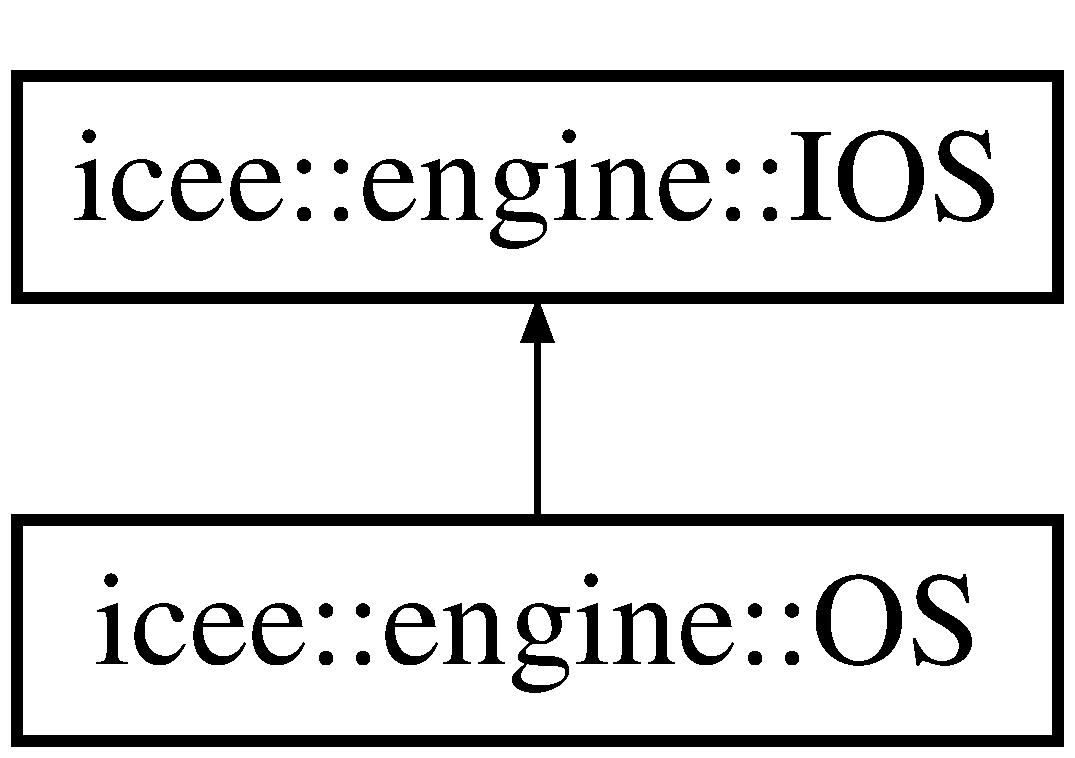
\includegraphics[height=2.000000cm]{classicee_1_1engine_1_1OS}
\end{center}
\end{figure}
\subsection*{Public Member Functions}
\begin{DoxyCompactItemize}
\item 
\hyperlink{classicee_1_1engine_1_1OS_ade94449836a8fce03cd44ed91c59e424}{OS} ()
\item 
virtual \hyperlink{classicee_1_1engine_1_1OS_a74ddb398eb3b33901a5294bbfa7f0fd2}{$\sim$OS} ()
\item 
virtual \hyperlink{namespacecompatibility_afc3ea6dfbdda98c9d2615b235b140a18}{sint32} \hyperlink{classicee_1_1engine_1_1OS_a42869381836268f3c27d610e43743da3}{initialize} ()
\item 
virtual \hyperlink{classicee_1_1engine_1_1IIceWindow}{IIceWindow} $\ast$ \hyperlink{classicee_1_1engine_1_1OS_a460645e9a18535546cecb2280cfe364e}{createWindow} (\hyperlink{namespacecompatibility_a51e8fe2956b4f39fe1fae96cec0d8393}{uint32} width=800, \hyperlink{namespacecompatibility_a51e8fe2956b4f39fe1fae96cec0d8393}{uint32} height=600, \hyperlink{namespacecompatibility_a51e8fe2956b4f39fe1fae96cec0d8393}{uint32} depth=24, bool fullscreen=false, bool vsync=false)
\end{DoxyCompactItemize}


\subsection{Constructor \& Destructor Documentation}
\hypertarget{classicee_1_1engine_1_1OS_ade94449836a8fce03cd44ed91c59e424}{
\index{icee::engine::OS@{icee::engine::OS}!OS@{OS}}
\index{OS@{OS}!icee::engine::OS@{icee::engine::OS}}
\subsubsection[{OS}]{\setlength{\rightskip}{0pt plus 5cm}icee::engine::OS::OS (
\begin{DoxyParamCaption}
{}
\end{DoxyParamCaption}
)}}
\label{classicee_1_1engine_1_1OS_ade94449836a8fce03cd44ed91c59e424}
Constructor. \hypertarget{classicee_1_1engine_1_1OS_a74ddb398eb3b33901a5294bbfa7f0fd2}{
\index{icee::engine::OS@{icee::engine::OS}!$\sim$OS@{$\sim$OS}}
\index{$\sim$OS@{$\sim$OS}!icee::engine::OS@{icee::engine::OS}}
\subsubsection[{$\sim$OS}]{\setlength{\rightskip}{0pt plus 5cm}icee::engine::OS::$\sim$OS (
\begin{DoxyParamCaption}
{}
\end{DoxyParamCaption}
)\hspace{0.3cm}{\ttfamily  \mbox{[}virtual\mbox{]}}}}
\label{classicee_1_1engine_1_1OS_a74ddb398eb3b33901a5294bbfa7f0fd2}
Destructor. 

\subsection{Member Function Documentation}
\hypertarget{classicee_1_1engine_1_1OS_a460645e9a18535546cecb2280cfe364e}{
\index{icee::engine::OS@{icee::engine::OS}!createWindow@{createWindow}}
\index{createWindow@{createWindow}!icee::engine::OS@{icee::engine::OS}}
\subsubsection[{createWindow}]{\setlength{\rightskip}{0pt plus 5cm}virtual {\bf IIceWindow}$\ast$ icee::engine::OS::createWindow (
\begin{DoxyParamCaption}
\item[{{\bf uint32}}]{width = {\ttfamily 800}, }
\item[{{\bf uint32}}]{height = {\ttfamily 600}, }
\item[{{\bf uint32}}]{depth = {\ttfamily 24}, }
\item[{bool}]{fullscreen = {\ttfamily false}, }
\item[{bool}]{vsync = {\ttfamily false}}
\end{DoxyParamCaption}
)\hspace{0.3cm}{\ttfamily  \mbox{[}inline, virtual\mbox{]}}}}
\label{classicee_1_1engine_1_1OS_a460645e9a18535546cecb2280cfe364e}


Implements \hyperlink{classicee_1_1engine_1_1IOS_a45a2101e58e5eb66774e717b26a343bb}{icee::engine::IOS}.

\hypertarget{classicee_1_1engine_1_1OS_a42869381836268f3c27d610e43743da3}{
\index{icee::engine::OS@{icee::engine::OS}!initialize@{initialize}}
\index{initialize@{initialize}!icee::engine::OS@{icee::engine::OS}}
\subsubsection[{initialize}]{\setlength{\rightskip}{0pt plus 5cm}virtual {\bf sint32} icee::engine::OS::initialize (
\begin{DoxyParamCaption}
{}
\end{DoxyParamCaption}
)\hspace{0.3cm}{\ttfamily  \mbox{[}inline, virtual\mbox{]}}}}
\label{classicee_1_1engine_1_1OS_a42869381836268f3c27d610e43743da3}


Implements \hyperlink{classicee_1_1engine_1_1IOS_aac944785a1b436e75b9f22881836ae75}{icee::engine::IOS}.



The documentation for this class was generated from the following files:\begin{DoxyCompactItemize}
\item 
src/engine/\hyperlink{OS_8h}{OS.h}\item 
src/engine/\hyperlink{OS_8cpp}{OS.cpp}\end{DoxyCompactItemize}

\hypertarget{classicee_1_1engine_1_1Quaternion}{
\section{icee::engine::Quaternion Class Reference}
\label{classicee_1_1engine_1_1Quaternion}\index{icee::engine::Quaternion@{icee::engine::Quaternion}}
}


{\ttfamily \#include $<$Quaternion.h$>$}

\subsection*{Public Member Functions}
\begin{DoxyCompactItemize}
\item 
\hyperlink{classicee_1_1engine_1_1Quaternion_af05d03b4ca06b0a4e321915ea1bc415f}{Quaternion} ()
\item 
\hyperlink{classicee_1_1engine_1_1Quaternion_a0efc38d80f6bca5de0b06dcc5aaa768d}{Quaternion} (\hyperlink{namespacecompatibility_a32a2d006ac2172c0f859370287f0104c}{float32} x, \hyperlink{namespacecompatibility_a32a2d006ac2172c0f859370287f0104c}{float32} y, \hyperlink{namespacecompatibility_a32a2d006ac2172c0f859370287f0104c}{float32} z, \hyperlink{namespacecompatibility_a32a2d006ac2172c0f859370287f0104c}{float32} real)
\item 
\hyperlink{classicee_1_1engine_1_1Quaternion_a6ab9de3854b0e2a1372313862aa7c867}{Quaternion} (const \hyperlink{classvmath_1_1Vector3f}{vmath::Vector3f} \&imaginary, \hyperlink{namespacecompatibility_a32a2d006ac2172c0f859370287f0104c}{float32} real)
\item 
void \hyperlink{classicee_1_1engine_1_1Quaternion_a76cddfcf2c2c2dcd55ff338f203d63a8}{buildFromAxisAngle} (\hyperlink{namespacecompatibility_a32a2d006ac2172c0f859370287f0104c}{float32} x, \hyperlink{namespacecompatibility_a32a2d006ac2172c0f859370287f0104c}{float32} y, \hyperlink{namespacecompatibility_a32a2d006ac2172c0f859370287f0104c}{float32} z, \hyperlink{namespacecompatibility_a32a2d006ac2172c0f859370287f0104c}{float32} angle)
\item 
\hyperlink{classicee_1_1engine_1_1Quaternion_addfb7d2ddf26bb468139758dbacfdb09}{Quaternion} (const \hyperlink{classicee_1_1engine_1_1Quaternion}{Quaternion} \&quat)
\item 
virtual \hyperlink{classicee_1_1engine_1_1Quaternion_af868c4f5ef7144e5c5b59895685034f3}{$\sim$Quaternion} ()
\item 
const \hyperlink{classicee_1_1engine_1_1Quaternion}{Quaternion} \& \hyperlink{classicee_1_1engine_1_1Quaternion_a68faa999336ddb833f942046973ead53}{operator=} (const \hyperlink{classicee_1_1engine_1_1Quaternion}{Quaternion} \&quat)
\item 
const \hyperlink{classicee_1_1engine_1_1Quaternion}{Quaternion} \hyperlink{classicee_1_1engine_1_1Quaternion_a7320af2f418e002be6fb4c02618b2003}{operator+} (const \hyperlink{classicee_1_1engine_1_1Quaternion}{Quaternion} \&quat) const 
\item 
const \hyperlink{classicee_1_1engine_1_1Quaternion}{Quaternion} \hyperlink{classicee_1_1engine_1_1Quaternion_a5c0407a4a5b3e1dcd0f34c2f58a4e863}{operator-\/} (const \hyperlink{classicee_1_1engine_1_1Quaternion}{Quaternion} \&quat) const 
\item 
const \hyperlink{classicee_1_1engine_1_1Quaternion}{Quaternion} \hyperlink{classicee_1_1engine_1_1Quaternion_ae74d3ee9e8a643ef88276fddd6d1ff48}{operator$\ast$} (const \hyperlink{classicee_1_1engine_1_1Quaternion}{Quaternion} \&quat) const 
\item 
const \hyperlink{classvmath_1_1Vector3f}{vmath::Vector3f} \hyperlink{classicee_1_1engine_1_1Quaternion_abc5ee696e09b025d38d513d7e106f0d7}{operator$\ast$} (const \hyperlink{classvmath_1_1Vector3f}{vmath::Vector3f} \&vec)
\item 
const \hyperlink{classicee_1_1engine_1_1Quaternion}{Quaternion} \hyperlink{classicee_1_1engine_1_1Quaternion_aeeec9056b9459d2d05060f735c8c23fc}{operator/} (const \hyperlink{classicee_1_1engine_1_1Quaternion}{Quaternion} \&quat) const 
\item 
const \hyperlink{classicee_1_1engine_1_1Quaternion}{Quaternion} \& \hyperlink{classicee_1_1engine_1_1Quaternion_a32a6406b0de790846aad43f0928cc4c4}{operator/=} (\hyperlink{namespacecompatibility_a32a2d006ac2172c0f859370287f0104c}{float32} scale)
\item 
void \hyperlink{classicee_1_1engine_1_1Quaternion_aaf51b47692013bf7a6495595f6d21533}{invert} ()
\item 
void \hyperlink{classicee_1_1engine_1_1Quaternion_a4e9d4d824905f6362220fa2c57e0e067}{conjugate} ()
\item 
\hyperlink{classicee_1_1engine_1_1Quaternion}{Quaternion} \hyperlink{classicee_1_1engine_1_1Quaternion_a9c232bebd7c401f462b10f091d957d4c}{getConjugate} ()
\item 
\hyperlink{namespacecompatibility_a32a2d006ac2172c0f859370287f0104c}{float32} \hyperlink{classicee_1_1engine_1_1Quaternion_a0eb2c4fdcaaaef963fe019ba788683a1}{length} () const 
\item 
\hyperlink{namespacecompatibility_a32a2d006ac2172c0f859370287f0104c}{float32} \hyperlink{classicee_1_1engine_1_1Quaternion_ac4cbb03886f6489404441cbcab9e18ad}{lengthSquared} ()
\item 
void \hyperlink{classicee_1_1engine_1_1Quaternion_acc40a99765d9cd15ad134d287702d648}{normalize} ()
\item 
void \hyperlink{classicee_1_1engine_1_1Quaternion_ade7147ca7516d59a194f075fe07b64d7}{fillMatrix} (\hyperlink{namespacecompatibility_a32a2d006ac2172c0f859370287f0104c}{float32} matrix\mbox{[}$\,$\mbox{]})
\end{DoxyCompactItemize}


\subsection{Constructor \& Destructor Documentation}
\hypertarget{classicee_1_1engine_1_1Quaternion_af05d03b4ca06b0a4e321915ea1bc415f}{
\index{icee::engine::Quaternion@{icee::engine::Quaternion}!Quaternion@{Quaternion}}
\index{Quaternion@{Quaternion}!icee::engine::Quaternion@{icee::engine::Quaternion}}
\subsubsection[{Quaternion}]{\setlength{\rightskip}{0pt plus 5cm}icee::engine::Quaternion::Quaternion (
\begin{DoxyParamCaption}
{}
\end{DoxyParamCaption}
)\hspace{0.3cm}{\ttfamily  \mbox{[}inline\mbox{]}}}}
\label{classicee_1_1engine_1_1Quaternion_af05d03b4ca06b0a4e321915ea1bc415f}
Constructor. \hypertarget{classicee_1_1engine_1_1Quaternion_a0efc38d80f6bca5de0b06dcc5aaa768d}{
\index{icee::engine::Quaternion@{icee::engine::Quaternion}!Quaternion@{Quaternion}}
\index{Quaternion@{Quaternion}!icee::engine::Quaternion@{icee::engine::Quaternion}}
\subsubsection[{Quaternion}]{\setlength{\rightskip}{0pt plus 5cm}icee::engine::Quaternion::Quaternion (
\begin{DoxyParamCaption}
\item[{{\bf float32}}]{x, }
\item[{{\bf float32}}]{y, }
\item[{{\bf float32}}]{z, }
\item[{{\bf float32}}]{real}
\end{DoxyParamCaption}
)\hspace{0.3cm}{\ttfamily  \mbox{[}inline\mbox{]}}}}
\label{classicee_1_1engine_1_1Quaternion_a0efc38d80f6bca5de0b06dcc5aaa768d}
Constructor. \hypertarget{classicee_1_1engine_1_1Quaternion_a6ab9de3854b0e2a1372313862aa7c867}{
\index{icee::engine::Quaternion@{icee::engine::Quaternion}!Quaternion@{Quaternion}}
\index{Quaternion@{Quaternion}!icee::engine::Quaternion@{icee::engine::Quaternion}}
\subsubsection[{Quaternion}]{\setlength{\rightskip}{0pt plus 5cm}icee::engine::Quaternion::Quaternion (
\begin{DoxyParamCaption}
\item[{const {\bf vmath::Vector3f} \&}]{imaginary, }
\item[{{\bf float32}}]{real}
\end{DoxyParamCaption}
)\hspace{0.3cm}{\ttfamily  \mbox{[}inline\mbox{]}}}}
\label{classicee_1_1engine_1_1Quaternion_a6ab9de3854b0e2a1372313862aa7c867}
Constructor. \hypertarget{classicee_1_1engine_1_1Quaternion_addfb7d2ddf26bb468139758dbacfdb09}{
\index{icee::engine::Quaternion@{icee::engine::Quaternion}!Quaternion@{Quaternion}}
\index{Quaternion@{Quaternion}!icee::engine::Quaternion@{icee::engine::Quaternion}}
\subsubsection[{Quaternion}]{\setlength{\rightskip}{0pt plus 5cm}icee::engine::Quaternion::Quaternion (
\begin{DoxyParamCaption}
\item[{const {\bf Quaternion} \&}]{quat}
\end{DoxyParamCaption}
)\hspace{0.3cm}{\ttfamily  \mbox{[}inline\mbox{]}}}}
\label{classicee_1_1engine_1_1Quaternion_addfb7d2ddf26bb468139758dbacfdb09}
Copy constructor. \hypertarget{classicee_1_1engine_1_1Quaternion_af868c4f5ef7144e5c5b59895685034f3}{
\index{icee::engine::Quaternion@{icee::engine::Quaternion}!$\sim$Quaternion@{$\sim$Quaternion}}
\index{$\sim$Quaternion@{$\sim$Quaternion}!icee::engine::Quaternion@{icee::engine::Quaternion}}
\subsubsection[{$\sim$Quaternion}]{\setlength{\rightskip}{0pt plus 5cm}virtual icee::engine::Quaternion::$\sim$Quaternion (
\begin{DoxyParamCaption}
{}
\end{DoxyParamCaption}
)\hspace{0.3cm}{\ttfamily  \mbox{[}inline, virtual\mbox{]}}}}
\label{classicee_1_1engine_1_1Quaternion_af868c4f5ef7144e5c5b59895685034f3}
Destructor. 

\subsection{Member Function Documentation}
\hypertarget{classicee_1_1engine_1_1Quaternion_a76cddfcf2c2c2dcd55ff338f203d63a8}{
\index{icee::engine::Quaternion@{icee::engine::Quaternion}!buildFromAxisAngle@{buildFromAxisAngle}}
\index{buildFromAxisAngle@{buildFromAxisAngle}!icee::engine::Quaternion@{icee::engine::Quaternion}}
\subsubsection[{buildFromAxisAngle}]{\setlength{\rightskip}{0pt plus 5cm}void icee::engine::Quaternion::buildFromAxisAngle (
\begin{DoxyParamCaption}
\item[{{\bf float32}}]{x, }
\item[{{\bf float32}}]{y, }
\item[{{\bf float32}}]{z, }
\item[{{\bf float32}}]{angle}
\end{DoxyParamCaption}
)\hspace{0.3cm}{\ttfamily  \mbox{[}inline\mbox{]}}}}
\label{classicee_1_1engine_1_1Quaternion_a76cddfcf2c2c2dcd55ff338f203d63a8}
Build this \hyperlink{classicee_1_1engine_1_1Quaternion}{Quaternion} from an axis angle. This is useful if you want to use the \hyperlink{classicee_1_1engine_1_1Quaternion}{Quaternion} to rotate through an angle about the axis (unit) vector. The equation for this is: q = cos(theta/2) + vector$\ast$sin(theta/2)


\begin{DoxyParams}{Parameters}
{\em x} & \\
\hline
{\em y} & \\
\hline
{\em z} & \\
\hline
{\em angle} & The angle, in radians \\
\hline
\end{DoxyParams}
\hypertarget{classicee_1_1engine_1_1Quaternion_a4e9d4d824905f6362220fa2c57e0e067}{
\index{icee::engine::Quaternion@{icee::engine::Quaternion}!conjugate@{conjugate}}
\index{conjugate@{conjugate}!icee::engine::Quaternion@{icee::engine::Quaternion}}
\subsubsection[{conjugate}]{\setlength{\rightskip}{0pt plus 5cm}void icee::engine::Quaternion::conjugate (
\begin{DoxyParamCaption}
{}
\end{DoxyParamCaption}
)\hspace{0.3cm}{\ttfamily  \mbox{[}inline\mbox{]}}}}
\label{classicee_1_1engine_1_1Quaternion_a4e9d4d824905f6362220fa2c57e0e067}
\hypertarget{classicee_1_1engine_1_1Quaternion_ade7147ca7516d59a194f075fe07b64d7}{
\index{icee::engine::Quaternion@{icee::engine::Quaternion}!fillMatrix@{fillMatrix}}
\index{fillMatrix@{fillMatrix}!icee::engine::Quaternion@{icee::engine::Quaternion}}
\subsubsection[{fillMatrix}]{\setlength{\rightskip}{0pt plus 5cm}void icee::engine::Quaternion::fillMatrix (
\begin{DoxyParamCaption}
\item[{{\bf float32}}]{matrix\mbox{[}$\,$\mbox{]}}
\end{DoxyParamCaption}
)\hspace{0.3cm}{\ttfamily  \mbox{[}inline\mbox{]}}}}
\label{classicee_1_1engine_1_1Quaternion_ade7147ca7516d59a194f075fe07b64d7}
Fills in Column-\/Major order. \hypertarget{classicee_1_1engine_1_1Quaternion_a9c232bebd7c401f462b10f091d957d4c}{
\index{icee::engine::Quaternion@{icee::engine::Quaternion}!getConjugate@{getConjugate}}
\index{getConjugate@{getConjugate}!icee::engine::Quaternion@{icee::engine::Quaternion}}
\subsubsection[{getConjugate}]{\setlength{\rightskip}{0pt plus 5cm}{\bf Quaternion} icee::engine::Quaternion::getConjugate (
\begin{DoxyParamCaption}
{}
\end{DoxyParamCaption}
)\hspace{0.3cm}{\ttfamily  \mbox{[}inline\mbox{]}}}}
\label{classicee_1_1engine_1_1Quaternion_a9c232bebd7c401f462b10f091d957d4c}
\hypertarget{classicee_1_1engine_1_1Quaternion_aaf51b47692013bf7a6495595f6d21533}{
\index{icee::engine::Quaternion@{icee::engine::Quaternion}!invert@{invert}}
\index{invert@{invert}!icee::engine::Quaternion@{icee::engine::Quaternion}}
\subsubsection[{invert}]{\setlength{\rightskip}{0pt plus 5cm}void icee::engine::Quaternion::invert (
\begin{DoxyParamCaption}
{}
\end{DoxyParamCaption}
)\hspace{0.3cm}{\ttfamily  \mbox{[}inline\mbox{]}}}}
\label{classicee_1_1engine_1_1Quaternion_aaf51b47692013bf7a6495595f6d21533}
\hypertarget{classicee_1_1engine_1_1Quaternion_a0eb2c4fdcaaaef963fe019ba788683a1}{
\index{icee::engine::Quaternion@{icee::engine::Quaternion}!length@{length}}
\index{length@{length}!icee::engine::Quaternion@{icee::engine::Quaternion}}
\subsubsection[{length}]{\setlength{\rightskip}{0pt plus 5cm}{\bf float32} icee::engine::Quaternion::length (
\begin{DoxyParamCaption}
{}
\end{DoxyParamCaption}
) const\hspace{0.3cm}{\ttfamily  \mbox{[}inline\mbox{]}}}}
\label{classicee_1_1engine_1_1Quaternion_a0eb2c4fdcaaaef963fe019ba788683a1}
\hypertarget{classicee_1_1engine_1_1Quaternion_ac4cbb03886f6489404441cbcab9e18ad}{
\index{icee::engine::Quaternion@{icee::engine::Quaternion}!lengthSquared@{lengthSquared}}
\index{lengthSquared@{lengthSquared}!icee::engine::Quaternion@{icee::engine::Quaternion}}
\subsubsection[{lengthSquared}]{\setlength{\rightskip}{0pt plus 5cm}{\bf float32} icee::engine::Quaternion::lengthSquared (
\begin{DoxyParamCaption}
{}
\end{DoxyParamCaption}
)\hspace{0.3cm}{\ttfamily  \mbox{[}inline\mbox{]}}}}
\label{classicee_1_1engine_1_1Quaternion_ac4cbb03886f6489404441cbcab9e18ad}
Get the squared length of this quaternion. \hypertarget{classicee_1_1engine_1_1Quaternion_acc40a99765d9cd15ad134d287702d648}{
\index{icee::engine::Quaternion@{icee::engine::Quaternion}!normalize@{normalize}}
\index{normalize@{normalize}!icee::engine::Quaternion@{icee::engine::Quaternion}}
\subsubsection[{normalize}]{\setlength{\rightskip}{0pt plus 5cm}void icee::engine::Quaternion::normalize (
\begin{DoxyParamCaption}
{}
\end{DoxyParamCaption}
)\hspace{0.3cm}{\ttfamily  \mbox{[}inline\mbox{]}}}}
\label{classicee_1_1engine_1_1Quaternion_acc40a99765d9cd15ad134d287702d648}
\hypertarget{classicee_1_1engine_1_1Quaternion_ae74d3ee9e8a643ef88276fddd6d1ff48}{
\index{icee::engine::Quaternion@{icee::engine::Quaternion}!operator$\ast$@{operator$\ast$}}
\index{operator$\ast$@{operator$\ast$}!icee::engine::Quaternion@{icee::engine::Quaternion}}
\subsubsection[{operator$\ast$}]{\setlength{\rightskip}{0pt plus 5cm}const {\bf Quaternion} icee::engine::Quaternion::operator$\ast$ (
\begin{DoxyParamCaption}
\item[{const {\bf Quaternion} \&}]{quat}
\end{DoxyParamCaption}
) const\hspace{0.3cm}{\ttfamily  \mbox{[}inline\mbox{]}}}}
\label{classicee_1_1engine_1_1Quaternion_ae74d3ee9e8a643ef88276fddd6d1ff48}
\hypertarget{classicee_1_1engine_1_1Quaternion_abc5ee696e09b025d38d513d7e106f0d7}{
\index{icee::engine::Quaternion@{icee::engine::Quaternion}!operator$\ast$@{operator$\ast$}}
\index{operator$\ast$@{operator$\ast$}!icee::engine::Quaternion@{icee::engine::Quaternion}}
\subsubsection[{operator$\ast$}]{\setlength{\rightskip}{0pt plus 5cm}const {\bf vmath::Vector3f} icee::engine::Quaternion::operator$\ast$ (
\begin{DoxyParamCaption}
\item[{const {\bf vmath::Vector3f} \&}]{vec}
\end{DoxyParamCaption}
)\hspace{0.3cm}{\ttfamily  \mbox{[}inline\mbox{]}}}}
\label{classicee_1_1engine_1_1Quaternion_abc5ee696e09b025d38d513d7e106f0d7}
\hypertarget{classicee_1_1engine_1_1Quaternion_a7320af2f418e002be6fb4c02618b2003}{
\index{icee::engine::Quaternion@{icee::engine::Quaternion}!operator+@{operator+}}
\index{operator+@{operator+}!icee::engine::Quaternion@{icee::engine::Quaternion}}
\subsubsection[{operator+}]{\setlength{\rightskip}{0pt plus 5cm}const {\bf Quaternion} icee::engine::Quaternion::operator+ (
\begin{DoxyParamCaption}
\item[{const {\bf Quaternion} \&}]{quat}
\end{DoxyParamCaption}
) const\hspace{0.3cm}{\ttfamily  \mbox{[}inline\mbox{]}}}}
\label{classicee_1_1engine_1_1Quaternion_a7320af2f418e002be6fb4c02618b2003}
\hypertarget{classicee_1_1engine_1_1Quaternion_a5c0407a4a5b3e1dcd0f34c2f58a4e863}{
\index{icee::engine::Quaternion@{icee::engine::Quaternion}!operator-\/@{operator-\/}}
\index{operator-\/@{operator-\/}!icee::engine::Quaternion@{icee::engine::Quaternion}}
\subsubsection[{operator-\/}]{\setlength{\rightskip}{0pt plus 5cm}const {\bf Quaternion} icee::engine::Quaternion::operator-\/ (
\begin{DoxyParamCaption}
\item[{const {\bf Quaternion} \&}]{quat}
\end{DoxyParamCaption}
) const\hspace{0.3cm}{\ttfamily  \mbox{[}inline\mbox{]}}}}
\label{classicee_1_1engine_1_1Quaternion_a5c0407a4a5b3e1dcd0f34c2f58a4e863}
\hypertarget{classicee_1_1engine_1_1Quaternion_aeeec9056b9459d2d05060f735c8c23fc}{
\index{icee::engine::Quaternion@{icee::engine::Quaternion}!operator/@{operator/}}
\index{operator/@{operator/}!icee::engine::Quaternion@{icee::engine::Quaternion}}
\subsubsection[{operator/}]{\setlength{\rightskip}{0pt plus 5cm}const {\bf Quaternion} icee::engine::Quaternion::operator/ (
\begin{DoxyParamCaption}
\item[{const {\bf Quaternion} \&}]{quat}
\end{DoxyParamCaption}
) const\hspace{0.3cm}{\ttfamily  \mbox{[}inline\mbox{]}}}}
\label{classicee_1_1engine_1_1Quaternion_aeeec9056b9459d2d05060f735c8c23fc}
\hypertarget{classicee_1_1engine_1_1Quaternion_a32a6406b0de790846aad43f0928cc4c4}{
\index{icee::engine::Quaternion@{icee::engine::Quaternion}!operator/=@{operator/=}}
\index{operator/=@{operator/=}!icee::engine::Quaternion@{icee::engine::Quaternion}}
\subsubsection[{operator/=}]{\setlength{\rightskip}{0pt plus 5cm}const {\bf Quaternion}\& icee::engine::Quaternion::operator/= (
\begin{DoxyParamCaption}
\item[{{\bf float32}}]{scale}
\end{DoxyParamCaption}
)\hspace{0.3cm}{\ttfamily  \mbox{[}inline\mbox{]}}}}
\label{classicee_1_1engine_1_1Quaternion_a32a6406b0de790846aad43f0928cc4c4}
\hypertarget{classicee_1_1engine_1_1Quaternion_a68faa999336ddb833f942046973ead53}{
\index{icee::engine::Quaternion@{icee::engine::Quaternion}!operator=@{operator=}}
\index{operator=@{operator=}!icee::engine::Quaternion@{icee::engine::Quaternion}}
\subsubsection[{operator=}]{\setlength{\rightskip}{0pt plus 5cm}const {\bf Quaternion}\& icee::engine::Quaternion::operator= (
\begin{DoxyParamCaption}
\item[{const {\bf Quaternion} \&}]{quat}
\end{DoxyParamCaption}
)\hspace{0.3cm}{\ttfamily  \mbox{[}inline\mbox{]}}}}
\label{classicee_1_1engine_1_1Quaternion_a68faa999336ddb833f942046973ead53}


The documentation for this class was generated from the following file:\begin{DoxyCompactItemize}
\item 
src/engine/\hyperlink{Quaternion_8h}{Quaternion.h}\end{DoxyCompactItemize}

\hypertarget{classTest}{
\section{Test Class Reference}
\label{classTest}\index{Test@{Test}}
}


{\ttfamily \#include $<$Test.h$>$}

\subsection*{Public Member Functions}
\begin{DoxyCompactItemize}
\item 
\hyperlink{classTest_a99f2bbfac6c95612322b0f10e607ebe5}{Test} ()
\item 
virtual \hyperlink{classTest_a2b0a62f1e667bbe8d8cb18d785bfa991}{$\sim$Test} ()
\item 
virtual void \hyperlink{classTest_a6b72d13434fbfbfb20036efd2eddb582}{receiveKeyboardEvent} (lwis::engine::KEYBOARD\_\-EVENT evt, lwis::engine::KEY key, \hyperlink{namespacecompatibility_a51e8fe2956b4f39fe1fae96cec0d8393}{uint32} mod, \hyperlink{namespacecompatibility_a451d9cfd3da606a663aa298356f0b5a5}{char8} character)
\item 
virtual void \hyperlink{classTest_ac74ca5b6a96ae120f185eb74faa83426}{receiveMouseEvent} (lwis::engine::MouseEvent evt)
\end{DoxyCompactItemize}
\subsection*{Static Public Attributes}
\begin{DoxyCompactItemize}
\item 
static \hyperlink{namespacecompatibility_a32a2d006ac2172c0f859370287f0104c}{float32} \hyperlink{classTest_ab43ab44c8f4ce5505edefd22fa88dbfb}{rotationX} = 0.0f
\item 
static \hyperlink{namespacecompatibility_a32a2d006ac2172c0f859370287f0104c}{float32} \hyperlink{classTest_a718270463659bee4d58f84cd85afa1d8}{rotationY} = 0.0f
\item 
static \hyperlink{namespacecompatibility_afc3ea6dfbdda98c9d2615b235b140a18}{sint32} \hyperlink{classTest_a480574c4cb8a857e5e9abc688b268d57}{mousePosX} = 0
\item 
static \hyperlink{namespacecompatibility_afc3ea6dfbdda98c9d2615b235b140a18}{sint32} \hyperlink{classTest_a69548f4b03e9b8193e5f460dd339a71e}{mousePosY} = 0
\item 
static bool \hyperlink{classTest_ab9b7c96eff4aa942c802e282201d2bef}{test} = false
\end{DoxyCompactItemize}


\subsection{Constructor \& Destructor Documentation}
\hypertarget{classTest_a99f2bbfac6c95612322b0f10e607ebe5}{
\index{Test@{Test}!Test@{Test}}
\index{Test@{Test}!Test@{Test}}
\subsubsection[{Test}]{\setlength{\rightskip}{0pt plus 5cm}Test::Test (
\begin{DoxyParamCaption}
{}
\end{DoxyParamCaption}
)}}
\label{classTest_a99f2bbfac6c95612322b0f10e607ebe5}
\hypertarget{classTest_a2b0a62f1e667bbe8d8cb18d785bfa991}{
\index{Test@{Test}!$\sim$Test@{$\sim$Test}}
\index{$\sim$Test@{$\sim$Test}!Test@{Test}}
\subsubsection[{$\sim$Test}]{\setlength{\rightskip}{0pt plus 5cm}Test::$\sim$Test (
\begin{DoxyParamCaption}
{}
\end{DoxyParamCaption}
)\hspace{0.3cm}{\ttfamily  \mbox{[}virtual\mbox{]}}}}
\label{classTest_a2b0a62f1e667bbe8d8cb18d785bfa991}


\subsection{Member Function Documentation}
\hypertarget{classTest_a6b72d13434fbfbfb20036efd2eddb582}{
\index{Test@{Test}!receiveKeyboardEvent@{receiveKeyboardEvent}}
\index{receiveKeyboardEvent@{receiveKeyboardEvent}!Test@{Test}}
\subsubsection[{receiveKeyboardEvent}]{\setlength{\rightskip}{0pt plus 5cm}void Test::receiveKeyboardEvent (
\begin{DoxyParamCaption}
\item[{lwis::engine::KEYBOARD\_\-EVENT}]{evt, }
\item[{lwis::engine::KEY}]{key, }
\item[{{\bf uint32}}]{mod, }
\item[{{\bf char8}}]{character}
\end{DoxyParamCaption}
)\hspace{0.3cm}{\ttfamily  \mbox{[}virtual\mbox{]}}}}
\label{classTest_a6b72d13434fbfbfb20036efd2eddb582}
\hypertarget{classTest_ac74ca5b6a96ae120f185eb74faa83426}{
\index{Test@{Test}!receiveMouseEvent@{receiveMouseEvent}}
\index{receiveMouseEvent@{receiveMouseEvent}!Test@{Test}}
\subsubsection[{receiveMouseEvent}]{\setlength{\rightskip}{0pt plus 5cm}void Test::receiveMouseEvent (
\begin{DoxyParamCaption}
\item[{lwis::engine::MouseEvent}]{evt}
\end{DoxyParamCaption}
)\hspace{0.3cm}{\ttfamily  \mbox{[}virtual\mbox{]}}}}
\label{classTest_ac74ca5b6a96ae120f185eb74faa83426}


\subsection{Member Data Documentation}
\hypertarget{classTest_a480574c4cb8a857e5e9abc688b268d57}{
\index{Test@{Test}!mousePosX@{mousePosX}}
\index{mousePosX@{mousePosX}!Test@{Test}}
\subsubsection[{mousePosX}]{\setlength{\rightskip}{0pt plus 5cm}{\bf sint32} {\bf Test::mousePosX} = 0\hspace{0.3cm}{\ttfamily  \mbox{[}static\mbox{]}}}}
\label{classTest_a480574c4cb8a857e5e9abc688b268d57}
\hypertarget{classTest_a69548f4b03e9b8193e5f460dd339a71e}{
\index{Test@{Test}!mousePosY@{mousePosY}}
\index{mousePosY@{mousePosY}!Test@{Test}}
\subsubsection[{mousePosY}]{\setlength{\rightskip}{0pt plus 5cm}{\bf sint32} {\bf Test::mousePosY} = 0\hspace{0.3cm}{\ttfamily  \mbox{[}static\mbox{]}}}}
\label{classTest_a69548f4b03e9b8193e5f460dd339a71e}
\hypertarget{classTest_ab43ab44c8f4ce5505edefd22fa88dbfb}{
\index{Test@{Test}!rotationX@{rotationX}}
\index{rotationX@{rotationX}!Test@{Test}}
\subsubsection[{rotationX}]{\setlength{\rightskip}{0pt plus 5cm}{\bf float32} {\bf Test::rotationX} = 0.0f\hspace{0.3cm}{\ttfamily  \mbox{[}static\mbox{]}}}}
\label{classTest_ab43ab44c8f4ce5505edefd22fa88dbfb}
\hypertarget{classTest_a718270463659bee4d58f84cd85afa1d8}{
\index{Test@{Test}!rotationY@{rotationY}}
\index{rotationY@{rotationY}!Test@{Test}}
\subsubsection[{rotationY}]{\setlength{\rightskip}{0pt plus 5cm}{\bf float32} {\bf Test::rotationY} = 0.0f\hspace{0.3cm}{\ttfamily  \mbox{[}static\mbox{]}}}}
\label{classTest_a718270463659bee4d58f84cd85afa1d8}
\hypertarget{classTest_ab9b7c96eff4aa942c802e282201d2bef}{
\index{Test@{Test}!test@{test}}
\index{test@{test}!Test@{Test}}
\subsubsection[{test}]{\setlength{\rightskip}{0pt plus 5cm}bool {\bf Test::test} = false\hspace{0.3cm}{\ttfamily  \mbox{[}static\mbox{]}}}}
\label{classTest_ab9b7c96eff4aa942c802e282201d2bef}


The documentation for this class was generated from the following files:\begin{DoxyCompactItemize}
\item 
src/\hyperlink{Test_8h}{Test.h}\item 
src/\hyperlink{Test_8cpp}{Test.cpp}\end{DoxyCompactItemize}

\hypertarget{classvmath_1_1Vector3f}{
\section{vmath::Vector3f Class Reference}
\label{classvmath_1_1Vector3f}\index{vmath::Vector3f@{vmath::Vector3f}}
}


{\ttfamily \#include $<$Vector3f.h$>$}

\subsection*{Public Member Functions}
\begin{DoxyCompactItemize}
\item 
\hyperlink{classvmath_1_1Vector3f_a72b542084cf068d21a0d6071cdd450ac}{Vector3f} (\hyperlink{namespacecompatibility_a32a2d006ac2172c0f859370287f0104c}{float32} \hyperlink{classvmath_1_1Vector3f_adfc960779db8a0dd2f9670af4d075a4a}{x}=0.f, \hyperlink{namespacecompatibility_a32a2d006ac2172c0f859370287f0104c}{float32} \hyperlink{classvmath_1_1Vector3f_a22cb6b05462c55b6d5475d37dbc667f4}{y}=0.f, \hyperlink{namespacecompatibility_a32a2d006ac2172c0f859370287f0104c}{float32} \hyperlink{classvmath_1_1Vector3f_ae4aaae3b4db7ef3c3e30d7c66cb9aa76}{z}=0.f)
\item 
\hyperlink{classvmath_1_1Vector3f_aa06734767f55fe5af3b33cde02c907e9}{Vector3f} (const \hyperlink{classvmath_1_1Vector3f}{Vector3f} \&v)
\item 
\hyperlink{classvmath_1_1Vector3f_a02ab79854d0661b6edf0cb76ef772c74}{$\sim$Vector3f} ()
\item 
const \hyperlink{classvmath_1_1Vector3f}{Vector3f} \& \hyperlink{classvmath_1_1Vector3f_aa274a0c0289461862613b355c77c8600}{operator$\ast$=} (const \hyperlink{namespacecompatibility_a32a2d006ac2172c0f859370287f0104c}{float32} \&f)
\item 
const \hyperlink{classvmath_1_1Vector3f}{Vector3f} \& \hyperlink{classvmath_1_1Vector3f_a07065d310608d9dbf27ee1bcb9b7cb5f}{operator/=} (const \hyperlink{namespacecompatibility_a32a2d006ac2172c0f859370287f0104c}{float32} \&f)
\item 
const \hyperlink{classvmath_1_1Vector3f}{Vector3f} \& \hyperlink{classvmath_1_1Vector3f_a7e23d7c01554d891030e12bd16b8a84e}{operator+=} (const \hyperlink{classvmath_1_1Vector3f}{Vector3f} \&vector)
\item 
const \hyperlink{classvmath_1_1Vector3f}{Vector3f} \hyperlink{classvmath_1_1Vector3f_ad04924bcee5ec66d7c4de7532c963bb0}{operator+} (const \hyperlink{classvmath_1_1Vector3f}{Vector3f} \&vector) const 
\item 
const \hyperlink{classvmath_1_1Vector3f}{Vector3f} \hyperlink{classvmath_1_1Vector3f_afb013ec02986559c48814dd61248e0bf}{operator-\/} (const \hyperlink{classvmath_1_1Vector3f}{Vector3f} \&vector) const 
\item 
const \hyperlink{namespacecompatibility_a32a2d006ac2172c0f859370287f0104c}{float32} \hyperlink{classvmath_1_1Vector3f_a8e95404bcc1cd481c0467daabc7898c4}{operator$\ast$} (const \hyperlink{classvmath_1_1Vector3f}{Vector3f} \&vector) const 
\item 
void \hyperlink{classvmath_1_1Vector3f_a0893f04b462cc37e960a4fdea3ba8e4d}{normalize} ()
\item 
const \hyperlink{namespacecompatibility_a32a2d006ac2172c0f859370287f0104c}{float32} \hyperlink{classvmath_1_1Vector3f_a33de43b35123995780b7fcc18ea21a58}{getLength} () const 
\end{DoxyCompactItemize}
\subsection*{Public Attributes}
\begin{DoxyCompactItemize}
\item 
\hyperlink{namespacecompatibility_a32a2d006ac2172c0f859370287f0104c}{float32} \hyperlink{classvmath_1_1Vector3f_adfc960779db8a0dd2f9670af4d075a4a}{x}
\item 
\hyperlink{namespacecompatibility_a32a2d006ac2172c0f859370287f0104c}{float32} \hyperlink{classvmath_1_1Vector3f_a22cb6b05462c55b6d5475d37dbc667f4}{y}
\item 
\hyperlink{namespacecompatibility_a32a2d006ac2172c0f859370287f0104c}{float32} \hyperlink{classvmath_1_1Vector3f_ae4aaae3b4db7ef3c3e30d7c66cb9aa76}{z}
\end{DoxyCompactItemize}


\subsection{Constructor \& Destructor Documentation}
\hypertarget{classvmath_1_1Vector3f_a72b542084cf068d21a0d6071cdd450ac}{
\index{vmath::Vector3f@{vmath::Vector3f}!Vector3f@{Vector3f}}
\index{Vector3f@{Vector3f}!vmath::Vector3f@{vmath::Vector3f}}
\subsubsection[{Vector3f}]{\setlength{\rightskip}{0pt plus 5cm}vmath::Vector3f::Vector3f (
\begin{DoxyParamCaption}
\item[{{\bf float32}}]{x = {\ttfamily 0.f}, }
\item[{{\bf float32}}]{y = {\ttfamily 0.f}, }
\item[{{\bf float32}}]{z = {\ttfamily 0.f}}
\end{DoxyParamCaption}
)}}
\label{classvmath_1_1Vector3f_a72b542084cf068d21a0d6071cdd450ac}
Basic constructor. \hypertarget{classvmath_1_1Vector3f_aa06734767f55fe5af3b33cde02c907e9}{
\index{vmath::Vector3f@{vmath::Vector3f}!Vector3f@{Vector3f}}
\index{Vector3f@{Vector3f}!vmath::Vector3f@{vmath::Vector3f}}
\subsubsection[{Vector3f}]{\setlength{\rightskip}{0pt plus 5cm}vmath::Vector3f::Vector3f (
\begin{DoxyParamCaption}
\item[{const {\bf Vector3f} \&}]{v}
\end{DoxyParamCaption}
)}}
\label{classvmath_1_1Vector3f_aa06734767f55fe5af3b33cde02c907e9}
Copy constructor. \hypertarget{classvmath_1_1Vector3f_a02ab79854d0661b6edf0cb76ef772c74}{
\index{vmath::Vector3f@{vmath::Vector3f}!$\sim$Vector3f@{$\sim$Vector3f}}
\index{$\sim$Vector3f@{$\sim$Vector3f}!vmath::Vector3f@{vmath::Vector3f}}
\subsubsection[{$\sim$Vector3f}]{\setlength{\rightskip}{0pt plus 5cm}vmath::Vector3f::$\sim$Vector3f (
\begin{DoxyParamCaption}
{}
\end{DoxyParamCaption}
)}}
\label{classvmath_1_1Vector3f_a02ab79854d0661b6edf0cb76ef772c74}


\subsection{Member Function Documentation}
\hypertarget{classvmath_1_1Vector3f_a33de43b35123995780b7fcc18ea21a58}{
\index{vmath::Vector3f@{vmath::Vector3f}!getLength@{getLength}}
\index{getLength@{getLength}!vmath::Vector3f@{vmath::Vector3f}}
\subsubsection[{getLength}]{\setlength{\rightskip}{0pt plus 5cm}const {\bf float32} vmath::Vector3f::getLength (
\begin{DoxyParamCaption}
{}
\end{DoxyParamCaption}
) const}}
\label{classvmath_1_1Vector3f_a33de43b35123995780b7fcc18ea21a58}
\hypertarget{classvmath_1_1Vector3f_a0893f04b462cc37e960a4fdea3ba8e4d}{
\index{vmath::Vector3f@{vmath::Vector3f}!normalize@{normalize}}
\index{normalize@{normalize}!vmath::Vector3f@{vmath::Vector3f}}
\subsubsection[{normalize}]{\setlength{\rightskip}{0pt plus 5cm}void vmath::Vector3f::normalize (
\begin{DoxyParamCaption}
{}
\end{DoxyParamCaption}
)}}
\label{classvmath_1_1Vector3f_a0893f04b462cc37e960a4fdea3ba8e4d}
\hypertarget{classvmath_1_1Vector3f_a8e95404bcc1cd481c0467daabc7898c4}{
\index{vmath::Vector3f@{vmath::Vector3f}!operator$\ast$@{operator$\ast$}}
\index{operator$\ast$@{operator$\ast$}!vmath::Vector3f@{vmath::Vector3f}}
\subsubsection[{operator$\ast$}]{\setlength{\rightskip}{0pt plus 5cm}const {\bf float32} vmath::Vector3f::operator$\ast$ (
\begin{DoxyParamCaption}
\item[{const {\bf Vector3f} \&}]{vector}
\end{DoxyParamCaption}
) const}}
\label{classvmath_1_1Vector3f_a8e95404bcc1cd481c0467daabc7898c4}
Overloaded $\ast$ operator (vector inner product). \hypertarget{classvmath_1_1Vector3f_aa274a0c0289461862613b355c77c8600}{
\index{vmath::Vector3f@{vmath::Vector3f}!operator$\ast$=@{operator$\ast$=}}
\index{operator$\ast$=@{operator$\ast$=}!vmath::Vector3f@{vmath::Vector3f}}
\subsubsection[{operator$\ast$=}]{\setlength{\rightskip}{0pt plus 5cm}const {\bf Vector3f} \& vmath::Vector3f::operator$\ast$= (
\begin{DoxyParamCaption}
\item[{const {\bf float32} \&}]{f}
\end{DoxyParamCaption}
)}}
\label{classvmath_1_1Vector3f_aa274a0c0289461862613b355c77c8600}
Overloaded $\ast$= operator. \hypertarget{classvmath_1_1Vector3f_ad04924bcee5ec66d7c4de7532c963bb0}{
\index{vmath::Vector3f@{vmath::Vector3f}!operator+@{operator+}}
\index{operator+@{operator+}!vmath::Vector3f@{vmath::Vector3f}}
\subsubsection[{operator+}]{\setlength{\rightskip}{0pt plus 5cm}const {\bf Vector3f} vmath::Vector3f::operator+ (
\begin{DoxyParamCaption}
\item[{const {\bf Vector3f} \&}]{vector}
\end{DoxyParamCaption}
) const}}
\label{classvmath_1_1Vector3f_ad04924bcee5ec66d7c4de7532c963bb0}
Overloaded + operator. \hypertarget{classvmath_1_1Vector3f_a7e23d7c01554d891030e12bd16b8a84e}{
\index{vmath::Vector3f@{vmath::Vector3f}!operator+=@{operator+=}}
\index{operator+=@{operator+=}!vmath::Vector3f@{vmath::Vector3f}}
\subsubsection[{operator+=}]{\setlength{\rightskip}{0pt plus 5cm}const {\bf Vector3f} \& vmath::Vector3f::operator+= (
\begin{DoxyParamCaption}
\item[{const {\bf Vector3f} \&}]{vector}
\end{DoxyParamCaption}
)}}
\label{classvmath_1_1Vector3f_a7e23d7c01554d891030e12bd16b8a84e}
Overloaded += operator. \hypertarget{classvmath_1_1Vector3f_afb013ec02986559c48814dd61248e0bf}{
\index{vmath::Vector3f@{vmath::Vector3f}!operator-\/@{operator-\/}}
\index{operator-\/@{operator-\/}!vmath::Vector3f@{vmath::Vector3f}}
\subsubsection[{operator-\/}]{\setlength{\rightskip}{0pt plus 5cm}const {\bf Vector3f} vmath::Vector3f::operator-\/ (
\begin{DoxyParamCaption}
\item[{const {\bf Vector3f} \&}]{vector}
\end{DoxyParamCaption}
) const}}
\label{classvmath_1_1Vector3f_afb013ec02986559c48814dd61248e0bf}
Overloaded -\/ operator. \hypertarget{classvmath_1_1Vector3f_a07065d310608d9dbf27ee1bcb9b7cb5f}{
\index{vmath::Vector3f@{vmath::Vector3f}!operator/=@{operator/=}}
\index{operator/=@{operator/=}!vmath::Vector3f@{vmath::Vector3f}}
\subsubsection[{operator/=}]{\setlength{\rightskip}{0pt plus 5cm}const {\bf Vector3f} \& vmath::Vector3f::operator/= (
\begin{DoxyParamCaption}
\item[{const {\bf float32} \&}]{f}
\end{DoxyParamCaption}
)}}
\label{classvmath_1_1Vector3f_a07065d310608d9dbf27ee1bcb9b7cb5f}
Overloaded /= operator. 

\subsection{Member Data Documentation}
\hypertarget{classvmath_1_1Vector3f_adfc960779db8a0dd2f9670af4d075a4a}{
\index{vmath::Vector3f@{vmath::Vector3f}!x@{x}}
\index{x@{x}!vmath::Vector3f@{vmath::Vector3f}}
\subsubsection[{x}]{\setlength{\rightskip}{0pt plus 5cm}{\bf float32} {\bf vmath::Vector3f::x}}}
\label{classvmath_1_1Vector3f_adfc960779db8a0dd2f9670af4d075a4a}
\hypertarget{classvmath_1_1Vector3f_a22cb6b05462c55b6d5475d37dbc667f4}{
\index{vmath::Vector3f@{vmath::Vector3f}!y@{y}}
\index{y@{y}!vmath::Vector3f@{vmath::Vector3f}}
\subsubsection[{y}]{\setlength{\rightskip}{0pt plus 5cm}{\bf float32} {\bf vmath::Vector3f::y}}}
\label{classvmath_1_1Vector3f_a22cb6b05462c55b6d5475d37dbc667f4}
\hypertarget{classvmath_1_1Vector3f_ae4aaae3b4db7ef3c3e30d7c66cb9aa76}{
\index{vmath::Vector3f@{vmath::Vector3f}!z@{z}}
\index{z@{z}!vmath::Vector3f@{vmath::Vector3f}}
\subsubsection[{z}]{\setlength{\rightskip}{0pt plus 5cm}{\bf float32} {\bf vmath::Vector3f::z}}}
\label{classvmath_1_1Vector3f_ae4aaae3b4db7ef3c3e30d7c66cb9aa76}


The documentation for this class was generated from the following files:\begin{DoxyCompactItemize}
\item 
src/vmath/\hyperlink{Vector3f_8h}{Vector3f.h}\item 
src/vmath/\hyperlink{Vector3f_8cpp}{Vector3f.cpp}\end{DoxyCompactItemize}

\chapter{File Documentation}
\hypertarget{Common_8h}{
\section{src/Common.h File Reference}
\label{Common_8h}\index{src/Common.h@{src/Common.h}}
}

\hypertarget{linux_2Common_8h}{
\section{src/linux/Common.h File Reference}
\label{linux_2Common_8h}\index{src/linux/Common.h@{src/linux/Common.h}}
}
{\ttfamily \#include \char`\"{}LinuxGLWindow.h\char`\"{}}\par
{\ttfamily \#include \char`\"{}OSLinux.h\char`\"{}}\par

\hypertarget{osx_2Common_8h}{
\section{src/osx/Common.h File Reference}
\label{osx_2Common_8h}\index{src/osx/Common.h@{src/osx/Common.h}}
}
{\ttfamily \#include \char`\"{}OSX.h\char`\"{}}\par
{\ttfamily \#include \char`\"{}OSXGLWindow.h\char`\"{}}\par

\hypertarget{windows_2Common_8h}{
\section{src/windows/Common.h File Reference}
\label{windows_2Common_8h}\index{src/windows/Common.h@{src/windows/Common.h}}
}
{\ttfamily \#include \char`\"{}OSWindows.h\char`\"{}}\par
{\ttfamily \#include \char`\"{}WindowsGLWindow.h\char`\"{}}\par

\hypertarget{Types_8h}{
\section{src/common/compatibility/Types.h File Reference}
\label{Types_8h}\index{src/common/compatibility/Types.h@{src/common/compatibility/Types.h}}
}
\subsection*{Namespaces}
\begin{DoxyCompactItemize}
\item 
namespace \hyperlink{namespacecompatibility}{compatibility}
\end{DoxyCompactItemize}
\subsection*{Typedefs}
\begin{DoxyCompactItemize}
\item 
typedef unsigned char \hyperlink{namespacecompatibility_a421e72ad468b7c7ffe74710a535b6ae0}{compatibility::uchar8}
\item 
typedef signed char \hyperlink{namespacecompatibility_a97718d4c4d671d147c6367c4aa8eaaaf}{compatibility::schar8}
\item 
typedef char \hyperlink{namespacecompatibility_a451d9cfd3da606a663aa298356f0b5a5}{compatibility::char8}
\item 
typedef unsigned short \hyperlink{namespacecompatibility_a54e2a2e111c7b0fe9641fa7afbee071d}{compatibility::uint16}
\item 
typedef signed short \hyperlink{namespacecompatibility_a55f18a31bf0e1572da9efb10a7b475fc}{compatibility::sint16}
\item 
typedef unsigned int \hyperlink{namespacecompatibility_a51e8fe2956b4f39fe1fae96cec0d8393}{compatibility::uint32}
\item 
typedef signed int \hyperlink{namespacecompatibility_afc3ea6dfbdda98c9d2615b235b140a18}{compatibility::sint32}
\item 
typedef float \hyperlink{namespacecompatibility_a32a2d006ac2172c0f859370287f0104c}{compatibility::float32}
\item 
typedef double \hyperlink{namespacecompatibility_ad1034b2c5db68564c02da8d500b21038}{compatibility::float64}
\end{DoxyCompactItemize}

\hypertarget{Math_8cpp}{
\section{src/common/math/Math.cpp File Reference}
\label{Math_8cpp}\index{src/common/math/Math.cpp@{src/common/math/Math.cpp}}
}
{\ttfamily \#include \char`\"{}Math.h\char`\"{}}\par
{\ttfamily \#include $<$math.h$>$}\par
{\ttfamily \#include $<$stdlib.h$>$}\par
\subsection*{Namespaces}
\begin{DoxyCompactItemize}
\item 
namespace \hyperlink{namespacemath}{math}
\end{DoxyCompactItemize}

\hypertarget{Math_8h}{\section{src/common/math/\-Math.h File Reference}
\label{Math_8h}\index{src/common/math/\-Math.\-h@{src/common/math/\-Math.\-h}}
}
\subsection*{Classes}
\begin{DoxyCompactItemize}
\item 
class \hyperlink{classmath_1_1Math}{math\-::\-Math}
\end{DoxyCompactItemize}
\subsection*{Namespaces}
\begin{DoxyCompactItemize}
\item 
namespace \hyperlink{namespacemath}{math}
\end{DoxyCompactItemize}
\subsection*{Variables}
\begin{DoxyCompactItemize}
\item 
static const float \hyperlink{namespacemath_a6bc2e46a09ced59adc7ca762c21672e9}{math\-::\-P\-I} = 3.\-14159265358979323846f
\item 
static const float \hyperlink{namespacemath_a4ec943d35c300759d313db7a5c9a28ca}{math\-::\-R\-E\-C\-I\-P\-R\-O\-C\-A\-L\-\_\-\-P\-I} = 1.\-0f / P\-I
\item 
static const float \hyperlink{namespacemath_ab0c0d4b652877ea23c84cbd2ceaba14f}{math\-::\-H\-A\-L\-F\-\_\-\-P\-I} = P\-I / 2.\-0f
\item 
static const float \hyperlink{namespacemath_a587d3c31fcbb87c5ccd1d9bb53a001ab}{math\-::\-D\-E\-G\-T\-O\-R\-A\-D} = P\-I / 180.\-0f
\item 
static const float \hyperlink{namespacemath_a16c58a21197921edbdf61706b7520088}{math\-::\-R\-A\-D\-T\-O\-D\-E\-G} = 180.\-0f / P\-I
\end{DoxyCompactItemize}

\hypertarget{Array_8h}{
\section{src/common/utilities/Array.h File Reference}
\label{Array_8h}\index{src/common/utilities/Array.h@{src/common/utilities/Array.h}}
}
{\ttfamily \#include \char`\"{}../compatibility/Types.h\char`\"{}}\par
{\ttfamily \#include \char`\"{}../math/Math.h\char`\"{}}\par
\subsection*{Classes}
\begin{DoxyCompactItemize}
\item 
class \hyperlink{classutilities_1_1Array}{utilities::Array$<$ T $>$}
\end{DoxyCompactItemize}
\subsection*{Namespaces}
\begin{DoxyCompactItemize}
\item 
namespace \hyperlink{namespaceutilities}{utilities}
\end{DoxyCompactItemize}

\hypertarget{CameraSceneNode_8cpp}{\section{src/\-Camera\-Scene\-Node.cpp File Reference}
\label{CameraSceneNode_8cpp}\index{src/\-Camera\-Scene\-Node.\-cpp@{src/\-Camera\-Scene\-Node.\-cpp}}
}
{\ttfamily \#include \char`\"{}glm/gtc/type\-\_\-ptr.\-hpp\char`\"{}}\\*
{\ttfamily \#include $<$glm/gtc/matrix\-\_\-transform.\-hpp$>$}\\*
{\ttfamily \#include $<$boost/log/trivial.\-hpp$>$}\\*
{\ttfamily \#include \char`\"{}Camera\-Scene\-Node.\-h\char`\"{}}\\*
{\ttfamily \#include \char`\"{}common/math/\-Math.\-h\char`\"{}}\\*
{\ttfamily \#include $<$G\-L/gl.\-h$>$}\\*
{\ttfamily \#include $<$iostream$>$}\\*
\subsection*{Namespaces}
\begin{DoxyCompactItemize}
\item 
namespace \hyperlink{namespaceoglre}{oglre}
\end{DoxyCompactItemize}

\hypertarget{CameraSceneNode_8h}{\section{src/\-Camera\-Scene\-Node.h File Reference}
\label{CameraSceneNode_8h}\index{src/\-Camera\-Scene\-Node.\-h@{src/\-Camera\-Scene\-Node.\-h}}
}
{\ttfamily \#include \char`\"{}glm/glm.\-hpp\char`\"{}}\\*
{\ttfamily \#include \char`\"{}glm/gtc/quaternion.\-hpp\char`\"{}}\\*
{\ttfamily \#include \char`\"{}I\-Camera.\-h\char`\"{}}\\*
{\ttfamily \#include \char`\"{}Default\-Scene\-Node.\-h\char`\"{}}\\*
\subsection*{Classes}
\begin{DoxyCompactItemize}
\item 
class \hyperlink{classoglre_1_1CameraSceneNode}{oglre\-::\-Camera\-Scene\-Node}
\end{DoxyCompactItemize}
\subsection*{Namespaces}
\begin{DoxyCompactItemize}
\item 
namespace \hyperlink{namespaceoglre}{oglre}
\end{DoxyCompactItemize}

\hypertarget{DefaultSceneManager_8cpp}{
\section{src/engine/DefaultSceneManager.cpp File Reference}
\label{DefaultSceneManager_8cpp}\index{src/engine/DefaultSceneManager.cpp@{src/engine/DefaultSceneManager.cpp}}
}
{\ttfamily \#include \char`\"{}DefaultSceneManager.h\char`\"{}}\par
{\ttfamily \#include \char`\"{}CameraSceneNode.h\char`\"{}}\par
{\ttfamily \#include \char`\"{}DefaultSceneNode.h\char`\"{}}\par
\subsection*{Namespaces}
\begin{DoxyCompactItemize}
\item 
namespace \hyperlink{namespaceicee}{icee}
\item 
namespace \hyperlink{namespaceicee_1_1engine}{icee::engine}
\end{DoxyCompactItemize}

\hypertarget{DefaultSceneManager_8h}{\section{src/\-Default\-Scene\-Manager.h File Reference}
\label{DefaultSceneManager_8h}\index{src/\-Default\-Scene\-Manager.\-h@{src/\-Default\-Scene\-Manager.\-h}}
}
{\ttfamily \#include \char`\"{}I\-Scene\-Manager.\-h\char`\"{}}\\*
{\ttfamily \#include \char`\"{}Camera\-Scene\-Node.\-h\char`\"{}}\\*
\subsection*{Classes}
\begin{DoxyCompactItemize}
\item 
class \hyperlink{classoglre_1_1DefaultSceneManager}{oglre\-::\-Default\-Scene\-Manager}
\end{DoxyCompactItemize}
\subsection*{Namespaces}
\begin{DoxyCompactItemize}
\item 
namespace \hyperlink{namespaceoglre}{oglre}
\end{DoxyCompactItemize}

\hypertarget{DefaultSceneNode_8cpp}{\section{src/\-Default\-Scene\-Node.cpp File Reference}
\label{DefaultSceneNode_8cpp}\index{src/\-Default\-Scene\-Node.\-cpp@{src/\-Default\-Scene\-Node.\-cpp}}
}
{\ttfamily \#include $<$stdlib.\-h$>$}\\*
{\ttfamily \#include $<$boost/log/trivial.\-hpp$>$}\\*
{\ttfamily \#include \char`\"{}Default\-Scene\-Node.\-h\char`\"{}}\\*
{\ttfamily \#include \char`\"{}shaders/\-Shader\-Program.\-h\char`\"{}}\\*
\subsection*{Namespaces}
\begin{DoxyCompactItemize}
\item 
namespace \hyperlink{namespaceoglre}{oglre}
\end{DoxyCompactItemize}

\hypertarget{DefaultSceneNode_8h}{\section{src/\-Default\-Scene\-Node.h File Reference}
\label{DefaultSceneNode_8h}\index{src/\-Default\-Scene\-Node.\-h@{src/\-Default\-Scene\-Node.\-h}}
}
{\ttfamily \#include $<$string$>$}\\*
{\ttfamily \#include \char`\"{}I\-Scene\-Node.\-h\char`\"{}}\\*
{\ttfamily \#include \char`\"{}shaders/\-I\-Shader\-Program.\-h\char`\"{}}\\*
{\ttfamily \#include \char`\"{}I\-Scene\-Manager.\-h\char`\"{}}\\*
\subsection*{Classes}
\begin{DoxyCompactItemize}
\item 
class \hyperlink{classoglre_1_1DefaultSceneNode}{oglre\-::\-Default\-Scene\-Node}
\end{DoxyCompactItemize}
\subsection*{Namespaces}
\begin{DoxyCompactItemize}
\item 
namespace \hyperlink{namespaceoglre}{oglre}
\end{DoxyCompactItemize}

\hypertarget{ICameraSceneNode_8h}{
\section{src/engine/ICameraSceneNode.h File Reference}
\label{ICameraSceneNode_8h}\index{src/engine/ICameraSceneNode.h@{src/engine/ICameraSceneNode.h}}
}
{\ttfamily \#include \char`\"{}ISceneNode.h\char`\"{}}\par
\subsection*{Classes}
\begin{DoxyCompactItemize}
\item 
class \hyperlink{classicee_1_1engine_1_1ICameraSceneNode}{icee::engine::ICameraSceneNode}
\end{DoxyCompactItemize}
\subsection*{Namespaces}
\begin{DoxyCompactItemize}
\item 
namespace \hyperlink{namespaceicee}{icee}
\item 
namespace \hyperlink{namespaceicee_1_1engine}{icee::engine}
\end{DoxyCompactItemize}

\hypertarget{IceEngineCommon_8h}{
\section{src/engine/IceEngineCommon.h File Reference}
\label{IceEngineCommon_8h}\index{src/engine/IceEngineCommon.h@{src/engine/IceEngineCommon.h}}
}
{\ttfamily \#include \char`\"{}IceGraphicsEngine.h\char`\"{}}\par
{\ttfamily \#include \char`\"{}IIceWindow.h\char`\"{}}\par
{\ttfamily \#include \char`\"{}ISceneManager.h\char`\"{}}\par
{\ttfamily \#include \char`\"{}ISceneNode.h\char`\"{}}\par
{\ttfamily \#include \char`\"{}ICameraSceneNode.h\char`\"{}}\par

\hypertarget{IceGLWindow_8cpp}{
\section{src/engine/IceGLWindow.cpp File Reference}
\label{IceGLWindow_8cpp}\index{src/engine/IceGLWindow.cpp@{src/engine/IceGLWindow.cpp}}
}
{\ttfamily \#include \char`\"{}IceGLWindow.h\char`\"{}}\par
{\ttfamily \#include \char`\"{}GL/glu.h\char`\"{}}\par
\subsection*{Namespaces}
\begin{DoxyCompactItemize}
\item 
namespace \hyperlink{namespaceicee}{icee}
\item 
namespace \hyperlink{namespaceicee_1_1engine}{icee::engine}
\end{DoxyCompactItemize}

\hypertarget{IceGLWindow_8h}{
\section{src/engine/IceGLWindow.h File Reference}
\label{IceGLWindow_8h}\index{src/engine/IceGLWindow.h@{src/engine/IceGLWindow.h}}
}
{\ttfamily \#include \char`\"{}IIceWindow.h\char`\"{}}\par
{\ttfamily \#include \char`\"{}DefaultSceneNode.h\char`\"{}}\par
{\ttfamily \#include \char`\"{}DefaultSceneManager.h\char`\"{}}\par
{\ttfamily \#include $<$GL/gl.h$>$}\par
\subsection*{Classes}
\begin{DoxyCompactItemize}
\item 
class \hyperlink{classicee_1_1engine_1_1IceGLWindow}{icee::engine::IceGLWindow}
\end{DoxyCompactItemize}
\subsection*{Namespaces}
\begin{DoxyCompactItemize}
\item 
namespace \hyperlink{namespaceicee}{icee}
\item 
namespace \hyperlink{namespaceicee_1_1engine}{icee::engine}
\end{DoxyCompactItemize}

\hypertarget{IceGraphicsEngine_8cpp}{
\section{src/engine/IceGraphicsEngine.cpp File Reference}
\label{IceGraphicsEngine_8cpp}\index{src/engine/IceGraphicsEngine.cpp@{src/engine/IceGraphicsEngine.cpp}}
}
{\ttfamily \#include \char`\"{}IceGraphicsEngine.h\char`\"{}}\par
\subsection*{Namespaces}
\begin{DoxyCompactItemize}
\item 
namespace \hyperlink{namespaceicee}{icee}
\item 
namespace \hyperlink{namespaceicee_1_1engine}{icee::engine}
\end{DoxyCompactItemize}

\hypertarget{IceGraphicsEngine_8h}{
\section{src/engine/IceGraphicsEngine.h File Reference}
\label{IceGraphicsEngine_8h}\index{src/engine/IceGraphicsEngine.h@{src/engine/IceGraphicsEngine.h}}
}
{\ttfamily \#include \char`\"{}IIceWindow.h\char`\"{}}\par
{\ttfamily \#include \char`\"{}IOS.h\char`\"{}}\par
\subsection*{Classes}
\begin{DoxyCompactItemize}
\item 
class \hyperlink{classicee_1_1engine_1_1IceGraphicsEngine}{icee::engine::IceGraphicsEngine}
\end{DoxyCompactItemize}
\subsection*{Namespaces}
\begin{DoxyCompactItemize}
\item 
namespace \hyperlink{namespaceicee}{icee}
\item 
namespace \hyperlink{namespaceicee_1_1engine}{icee::engine}
\end{DoxyCompactItemize}

\hypertarget{IIceWindow_8h}{
\section{src/engine/IIceWindow.h File Reference}
\label{IIceWindow_8h}\index{src/engine/IIceWindow.h@{src/engine/IIceWindow.h}}
}
{\ttfamily \#include \char`\"{}../common/compatibility/Types.h\char`\"{}}\par
{\ttfamily \#include \char`\"{}ISceneManager.h\char`\"{}}\par
{\ttfamily \#include $<$string$>$}\par
\subsection*{Classes}
\begin{DoxyCompactItemize}
\item 
class \hyperlink{classicee_1_1engine_1_1IIceWindow}{icee::engine::IIceWindow}
\end{DoxyCompactItemize}
\subsection*{Namespaces}
\begin{DoxyCompactItemize}
\item 
namespace \hyperlink{namespaceicee}{icee}
\item 
namespace \hyperlink{namespaceicee_1_1engine}{icee::engine}
\end{DoxyCompactItemize}

\hypertarget{IMesh_8h}{
\section{src/engine/IMesh.h File Reference}
\label{IMesh_8h}\index{src/engine/IMesh.h@{src/engine/IMesh.h}}
}
\subsection*{Classes}
\begin{DoxyCompactItemize}
\item 
class \hyperlink{classicee_1_1engine_1_1IMesh}{icee::engine::IMesh}
\end{DoxyCompactItemize}
\subsection*{Namespaces}
\begin{DoxyCompactItemize}
\item 
namespace \hyperlink{namespaceicee}{icee}
\item 
namespace \hyperlink{namespaceicee_1_1engine}{icee::engine}
\end{DoxyCompactItemize}

\hypertarget{IOS_8h}{
\section{src/engine/IOS.h File Reference}
\label{IOS_8h}\index{src/engine/IOS.h@{src/engine/IOS.h}}
}
{\ttfamily \#include \char`\"{}IIceWindow.h\char`\"{}}\par
{\ttfamily \#include \char`\"{}ISceneManager.h\char`\"{}}\par
{\ttfamily \#include \char`\"{}../common/compatibility/Types.h\char`\"{}}\par
\subsection*{Classes}
\begin{DoxyCompactItemize}
\item 
class \hyperlink{classicee_1_1engine_1_1IOS}{icee::engine::IOS}
\end{DoxyCompactItemize}
\subsection*{Namespaces}
\begin{DoxyCompactItemize}
\item 
namespace \hyperlink{namespaceicee}{icee}
\item 
namespace \hyperlink{namespaceicee_1_1engine}{icee::engine}
\end{DoxyCompactItemize}

\hypertarget{ISceneManager_8h}{\section{src/\-I\-Scene\-Manager.h File Reference}
\label{ISceneManager_8h}\index{src/\-I\-Scene\-Manager.\-h@{src/\-I\-Scene\-Manager.\-h}}
}
{\ttfamily \#include \char`\"{}I\-Scene\-Node.\-h\char`\"{}}\\*
{\ttfamily \#include \char`\"{}I\-Camera.\-h\char`\"{}}\\*
{\ttfamily \#include \char`\"{}I\-Light.\-h\char`\"{}}\\*
{\ttfamily \#include \char`\"{}models/\-I\-Model\-Manager.\-h\char`\"{}}\\*
{\ttfamily \#include \char`\"{}shaders/\-I\-Shader\-Program\-Manager.\-h\char`\"{}}\\*
\subsection*{Classes}
\begin{DoxyCompactItemize}
\item 
class \hyperlink{classoglre_1_1ISceneManager}{oglre\-::\-I\-Scene\-Manager}
\end{DoxyCompactItemize}
\subsection*{Namespaces}
\begin{DoxyCompactItemize}
\item 
namespace \hyperlink{namespaceoglre}{oglre}
\end{DoxyCompactItemize}

\hypertarget{ISceneNode_8h}{\section{src/\-I\-Scene\-Node.h File Reference}
\label{ISceneNode_8h}\index{src/\-I\-Scene\-Node.\-h@{src/\-I\-Scene\-Node.\-h}}
}
{\ttfamily \#include $<$vector$>$}\\*
{\ttfamily \#include $<$glm/glm.\-hpp$>$}\\*
{\ttfamily \#include \char`\"{}glm/gtc/quaternion.\-hpp\char`\"{}}\\*
{\ttfamily \#include \char`\"{}models/\-I\-Model.\-h\char`\"{}}\\*
\subsection*{Classes}
\begin{DoxyCompactItemize}
\item 
class \hyperlink{classglr_1_1ISceneNode}{glr\-::\-I\-Scene\-Node}
\end{DoxyCompactItemize}
\subsection*{Namespaces}
\begin{DoxyCompactItemize}
\item 
namespace \hyperlink{namespaceglr}{glr}
\end{DoxyCompactItemize}

\hypertarget{OS_8cpp}{
\section{src/engine/OS.cpp File Reference}
\label{OS_8cpp}\index{src/engine/OS.cpp@{src/engine/OS.cpp}}
}
{\ttfamily \#include \char`\"{}OS.h\char`\"{}}\par
\subsection*{Namespaces}
\begin{DoxyCompactItemize}
\item 
namespace \hyperlink{namespaceicee}{icee}
\item 
namespace \hyperlink{namespaceicee_1_1engine}{icee::engine}
\end{DoxyCompactItemize}

\hypertarget{OS_8h}{
\section{src/engine/OS.h File Reference}
\label{OS_8h}\index{src/engine/OS.h@{src/engine/OS.h}}
}
{\ttfamily \#include \char`\"{}IOS.h\char`\"{}}\par
{\ttfamily \#include \char`\"{}DefaultSceneManager.h\char`\"{}}\par
\subsection*{Classes}
\begin{DoxyCompactItemize}
\item 
class \hyperlink{classicee_1_1engine_1_1OS}{icee::engine::OS}
\end{DoxyCompactItemize}
\subsection*{Namespaces}
\begin{DoxyCompactItemize}
\item 
namespace \hyperlink{namespaceicee}{icee}
\item 
namespace \hyperlink{namespaceicee_1_1engine}{icee::engine}
\end{DoxyCompactItemize}

\hypertarget{Quaternion_8h}{
\section{src/engine/Quaternion.h File Reference}
\label{Quaternion_8h}\index{src/engine/Quaternion.h@{src/engine/Quaternion.h}}
}
{\ttfamily \#include \char`\"{}../vmath/Vector3f.h\char`\"{}}\par
{\ttfamily \#include \char`\"{}../common/math/Math.h\char`\"{}}\par
{\ttfamily \#include $<$math.h$>$}\par
\subsection*{Classes}
\begin{DoxyCompactItemize}
\item 
class \hyperlink{classicee_1_1engine_1_1Quaternion}{icee::engine::Quaternion}
\end{DoxyCompactItemize}
\subsection*{Namespaces}
\begin{DoxyCompactItemize}
\item 
namespace \hyperlink{namespaceicee}{icee}
\item 
namespace \hyperlink{namespaceicee_1_1engine}{icee::engine}
\end{DoxyCompactItemize}

\hypertarget{LinuxGLWindow_8cpp}{
\section{src/linux/LinuxGLWindow.cpp File Reference}
\label{LinuxGLWindow_8cpp}\index{src/linux/LinuxGLWindow.cpp@{src/linux/LinuxGLWindow.cpp}}
}

\hypertarget{LinuxGLWindow_8h}{
\section{src/linux/LinuxGLWindow.h File Reference}
\label{LinuxGLWindow_8h}\index{src/linux/LinuxGLWindow.h@{src/linux/LinuxGLWindow.h}}
}

\hypertarget{OSLinux_8cpp}{
\section{src/linux/OSLinux.cpp File Reference}
\label{OSLinux_8cpp}\index{src/linux/OSLinux.cpp@{src/linux/OSLinux.cpp}}
}

\hypertarget{OSLinux_8h}{
\section{src/linux/OSLinux.h File Reference}
\label{OSLinux_8h}\index{src/linux/OSLinux.h@{src/linux/OSLinux.h}}
}

\hypertarget{OSX_8cpp}{
\section{src/osx/OSX.cpp File Reference}
\label{OSX_8cpp}\index{src/osx/OSX.cpp@{src/osx/OSX.cpp}}
}

\hypertarget{OSX_8h}{
\section{src/osx/OSX.h File Reference}
\label{OSX_8h}\index{src/osx/OSX.h@{src/osx/OSX.h}}
}

\hypertarget{OSXGLWindow_8cpp}{
\section{src/osx/OSXGLWindow.cpp File Reference}
\label{OSXGLWindow_8cpp}\index{src/osx/OSXGLWindow.cpp@{src/osx/OSXGLWindow.cpp}}
}

\hypertarget{OSXGLWindow_8h}{
\section{src/osx/OSXGLWindow.h File Reference}
\label{OSXGLWindow_8h}\index{src/osx/OSXGLWindow.h@{src/osx/OSXGLWindow.h}}
}

\hypertarget{Test_8cpp}{
\section{src/Test.cpp File Reference}
\label{Test_8cpp}\index{src/Test.cpp@{src/Test.cpp}}
}
{\ttfamily \#include \char`\"{}Test.h\char`\"{}}\par
{\ttfamily \#include \char`\"{}engine/IceEngineCommon.h\char`\"{}}\par
{\ttfamily \#include $<$iostream$>$}\par
\subsection*{Functions}
\begin{DoxyCompactItemize}
\item 
int \hyperlink{Test_8cpp_ae66f6b31b5ad750f1fe042a706a4e3d4}{main} ()
\end{DoxyCompactItemize}


\subsection{Function Documentation}
\hypertarget{Test_8cpp_ae66f6b31b5ad750f1fe042a706a4e3d4}{
\index{Test.cpp@{Test.cpp}!main@{main}}
\index{main@{main}!Test.cpp@{Test.cpp}}
\subsubsection[{main}]{\setlength{\rightskip}{0pt plus 5cm}int main (
\begin{DoxyParamCaption}
{}
\end{DoxyParamCaption}
)}}
\label{Test_8cpp_ae66f6b31b5ad750f1fe042a706a4e3d4}

\hypertarget{Test_8h}{
\section{src/Test.h File Reference}
\label{Test_8h}\index{src/Test.h@{src/Test.h}}
}
{\ttfamily \#include \char`\"{}LWISCommon.h\char`\"{}}\par
\subsection*{Classes}
\begin{DoxyCompactItemize}
\item 
class \hyperlink{classTest}{Test}
\end{DoxyCompactItemize}

\hypertarget{Vector3f_8cpp}{
\section{src/vmath/Vector3f.cpp File Reference}
\label{Vector3f_8cpp}\index{src/vmath/Vector3f.cpp@{src/vmath/Vector3f.cpp}}
}
{\ttfamily \#include \char`\"{}Vector3f.h\char`\"{}}\par
{\ttfamily \#include $<$math.h$>$}\par
\subsection*{Namespaces}
\begin{DoxyCompactItemize}
\item 
namespace \hyperlink{namespacevmath}{vmath}
\end{DoxyCompactItemize}

\hypertarget{Vector3f_8h}{
\section{src/vmath/Vector3f.h File Reference}
\label{Vector3f_8h}\index{src/vmath/Vector3f.h@{src/vmath/Vector3f.h}}
}
{\ttfamily \#include \char`\"{}../common/compatibility/Types.h\char`\"{}}\par
\subsection*{Classes}
\begin{DoxyCompactItemize}
\item 
class \hyperlink{classvmath_1_1Vector3f}{vmath::Vector3f}
\end{DoxyCompactItemize}
\subsection*{Namespaces}
\begin{DoxyCompactItemize}
\item 
namespace \hyperlink{namespacevmath}{vmath}
\end{DoxyCompactItemize}

\hypertarget{OSWindows_8cpp}{
\section{src/windows/OSWindows.cpp File Reference}
\label{OSWindows_8cpp}\index{src/windows/OSWindows.cpp@{src/windows/OSWindows.cpp}}
}

\hypertarget{OSWindows_8h}{
\section{src/windows/OSWindows.h File Reference}
\label{OSWindows_8h}\index{src/windows/OSWindows.h@{src/windows/OSWindows.h}}
}

\hypertarget{WindowsGLWindow_8cpp}{
\section{src/windows/WindowsGLWindow.cpp File Reference}
\label{WindowsGLWindow_8cpp}\index{src/windows/WindowsGLWindow.cpp@{src/windows/WindowsGLWindow.cpp}}
}

\hypertarget{WindowsGLWindow_8h}{
\section{src/windows/WindowsGLWindow.h File Reference}
\label{WindowsGLWindow_8h}\index{src/windows/WindowsGLWindow.h@{src/windows/WindowsGLWindow.h}}
}

\printindex
\end{document}
